

\documentclass[a4paper,12pt]{article}
 \usepackage[stable]{footmisc}

%\usepackage{bracket}
\usepackage[margin=0.40 in]{geometry}
\usepackage{wrapfig}
\usepackage{etex}
\usepackage[T1]{fontenc}
\newcommand{\eva}[2]{\left.#1\right|_{#2}}
\usepackage{biblatex}
\usepackage[utf8]{inputenc}
\usepackage[italian]{babel}
\usepackage[pdftex]{graphicx}
\usepackage{braket}
\usepackage[usenames,dvipsnames,x11names]{xcolor}
\usepackage{microtype}
\usepackage{amsmath}
\usepackage{mathrsfs}
\usepackage{caption}
\usepackage{color}
\usepackage[separate-uncertainty = true]{siunitx}
\usepackage{amsmath}
\usepackage{amssymb}
\usepackage{amsfonts}
\usepackage{amsthm}
\usepackage{booktabs}
\usepackage{paralist}
\usepackage{subfig}
\usepackage{array}
\usepackage{xy}
\usepackage{multicol}
\usepackage{physics}
\usepackage{fancyhdr}
\usepackage{makeidx}
\usepackage{hyperref}
\usepackage{wrapfig}
\usepackage[T1,OT1]{fontenc} 
\usepackage{chemfig}
\usepackage{epigraph}
\usepackage{textcomp}
\usepackage[makeroom]{cancel}
\usepackage{enumitem}
\usepackage{braket}
\usepackage{pgfplots}
\usepackage[thinc]{esdiff}
\usepackage{grffile}
\usepackage{tikz}
\usepackage{pgf} 
\usepackage{MnSymbol,wasysym}
\usepackage{empheq}
\usepackage{xcolor}
\definecolor{lightgreen}{HTML}{90EE90}
\renewcommand{\arg}[1]{_{(#1)}}
\newcommand{\boxedeq}[2]{\begin{empheq}[box={\fboxsep=6pt\fbox}]{align}\label{#1}#2\end{empheq}}
\newcommand{\coloredeq}[2]{\begin{empheq}[box=\colorbox{lightgreen}]{align}\label{#1}#2\end{empheq}}
\usetikzlibrary{shapes.geometric,calc,matrix,arrows,snakes,shapes,patterns}
\theoremstyle{plain}

\renewcommand{\vec}[1]{{\boldsymbol{#1}}}
\newtheorem{thm}{Teorema}[section]
\newtheorem{lem}[thm]{Lemma}
\newtheorem{prop}[thm]{Proposizione}
\newtheorem{post}[thm]{Postulato}
\newtheorem{cor}[thm]{Corollario}
\theoremstyle{definition}
\newtheorem{defn}{Definizione}[section]
\newtheorem{exmp}{Esempio}[section]
\newtheorem{prob}{Problema}[section]
\newtheorem{hint}{Suggerimento}[section]
\newtheorem{sol}{Soluzione}[section]
\usepackage{mdframed}
\newmdtheoremenv{obs}{Fatto}

\newcommand{\Op}[1]{\mathcal{#1}}
\newcommand{\Dhil}{\sigma(\mathscr{H})}
\newcommand{\Hil}{\mathscr{H}}
\newcommand{\dif}{\mathrm{d}}
\newcommand{\Aop}{\mathcal{A}}
\newcommand{\Bop}{\mathcal{B}}
\newcommand{\Uop}{\mathcal{U}}
\newcommand{\Jop}{\mathcal{J}}
\newcommand{\Kop}{\mathcal{K}}
\newcommand{\Mop}{\mathcal{M}}
\newcommand{\Eop}{\mathcal{E}}
\newcommand{\Ker}{\mathrhm{Ker}}
\newcommand{\ifandonlyif}{\Longleftrightarrow}
\newcommand{\dagg}{^\dagger}
\newcommand{\f}[2]{\frac{#1}{#2}}
\newcommand{\ave}[1]{\left\langle#1\right\rangle }
\newcommand{\kst}{\ket{\Psi}}
\newcommand{\lkst}{\ket{\psi}}
\newcommand{\likst}{\ket{\psi_i}}
\newcommand{\lbst}{\bra{\psi}}
\newcommand{\libst}{\bra{\psi_i}}
\DeclareRobustCommand{\rchi}{{\mathpalette\irchi\relax}}
\newcommand{\irchi}[2]{\raisebox{\depth}{$#1\chi$}} % inner command, used by \rchi
\newcommand{\ikst}{\ket{\Psi_i}}
\newcommand{\zkst}{\ket{0}}
\newcommand{\okst}{\ket{1}}
\newcommand{\zbst}{\bra{0}}
\newcommand{\obst}{\bra{1}}
\newcommand{\bst}{\bra{\Psi}}
\newcommand{\ibst}{\bra{\Psi_i}}
\newcommand{\Ast}{\rho_A}
\newcommand{\Bst}{\rho_B}
\newcommand{\tdv}{\partial_t}

\newcommand{\kvec}{\vec{k}}
\newcommand{\Bhil}{\mathscr{H}_B}
\newcommand{\Var}{\mathrm{Var}}
\renewcommand{\var}[1]{\mathrm{Var}\left(#1\right)}
\renewcommand{\d}{\text{d}}
\newcommand{\openE}{\mathord{\mathchoice
		{\do@openE\tf@size}
		{\do@openE\tf@size}
		{\do@openE\sf@size}
		{\do@openE\ssf@size}
}}
\newcommand{\econg}{~\text{e}~}
\newcommand{\sint}{{S}\int}
\newcommand{\Shil}{\mathscr{H}_S}
\newcommand{\Ahil}{\mathscr{H}_A}
\renewcommand{\unit}{\text{Id}}
\newcommand{\pos}{\vec{x}}
\newcommand{\rpos}{\vec{r}}
\newcommand{\shcro}{Schrödinger }
\newcommand{\mom}{\vec{p}}
\newcommand{\bol}{k_b }
\newcommand{\tem}{k_b T }
\newcommand{\gw}[1]{\arg{#1}}
\newcommand{\argg}[1]{\left(#1\right)}
\ExplSyntaxOn
\NewDocumentCommand{\cycle}{ O{\;} m }
{
	(
	\alec_cycle:nn { #1 } { #2 }
	)
}

\seq_new:N \l_alec_cycle_seq
\cs_new_protected:Npn \alec_cycle:nn #1 #2
{
	\seq_set_split:Nnn \l_alec_cycle_seq { , } { #2 }
	\seq_use:Nn \l_alec_cycle_seq { #1 }
}
\ExplSyntaxOff
\newcommand{\efield}{\vec{E}}
\newcommand{\ra}{\rightarrow}
\newcommand{\qpl}{2\pi \hbar}
\theoremstyle{remark}
\newtheorem*{note}{Nota}
\title{Appunti del corso di Sistemi Complessi}
\addbibresource{biblio.bib}
\author{ Alessandro Foligno}

\begin{document}
	\tableofcontents
	\part{Statistica}\footnote{In gran parte ispirato da: "Stochastic Methods: A Handbook for the Natural and Social, Gardiner"}


	\section{Definizione astratta di Probabilità}
	Quando si vuole parlare di probabilità di un evento, questo è parte di un insieme più grande, l'insieme di tutti gli eventi possibili.\\
	
	Uno spazio di probabilità è una tripla $(\Omega,\Op{F},\mu)$ dove $\Omega$ è il \textbf{sample space}, che racchiude i possibili risultati (ad esempio testa/croce per una moneta, posizione per una particella, ecc), $\Op{F}$ è l'insieme degli eventi, ovvero i suoi elementi sono sottoinsiemi di $\Omega$ che rappresentano l'informazione sul sistema (ad esempio è uscito un numero pari da un dado, oppure il numero di testa è uguale al numero di croce), e $\mu$ è una misura che assegna ad ogni $A\in \Op{F}$ una probabilità $P$ che rispetta alcuni assiomi.\\In particolare $\Op{F}$ non è l'insieme delle parti di $\Omega$ (è vero solo per $\Omega$ finiti o numerabili), ma ad esempio l'algebra di Borel di $\Omega$ (perchè è possibile definirci sopra una misura)
	\subsection{Assiomi}

	\begin{itemize}
		\item $P\arg{A}\ge0$
		\item $P\arg{\Omega}=1$
		\item Se $\{A_i\}_{i\in \mathbb{N}}$ è una collezione di sottoinsiemi di $\Omega$, \textbf{al più numerabile} e ogni coppia di insiemi non ha elementi in comune (cioè $\forall (i,j)\in \mathbb{N}^2 \implies A_i \cap A_j=\O$) allora deve valere:
		\[P\left({\cup_i A_i}\right)=\sum_i P\arg{A_i}		\]
		Ovvero che la probabilità che avvenga uno degli eventi contenuto nei vari insiemi, sia la somma delle probabilità
	\end{itemize}
	Una semplice conseguenza di questi assiomi è, considerando un insieme e il suo complementare $\bar{A}=\Omega\setminus A$ (che hanno intersezione vuota, quindi è possibile applicare il terzo assioma):
	\[P\arg{A}+	P\arg{\bar{A}}=P\arg{\Omega}=1\implies P\arg{\bar{A}}=1-P\arg{A}	\]
	Il motivo per cui il terzo assioma richiede che la probabilità si sommi solo su una collezione numerabile di insiemi è presto giustificato. Ad esempio considerando come eventi i numeri reali\[x\in[0,1]\] con probabilità uniforme,
	si ha che un singolo punto ha probabilità $0$ di essere scelto. Tuttavia, un unione non numerabile di punti, come ad esempio tutto l'intervallo, non ha probabilità nulla di essere scelta (come succederebbe se si sommassero le probabilità nulle dei singoli punti).
	
\begin{obs}\label{abuso1}
Siano $\{B_i\}_{i\in I }$ dei set di eventi tali che \[\bigcup_{I} B_i=\Omega\]
\[B_i\cap B_j=\emptyset\]
Allora vale che 
\[P\arg{A}=P\arg{A\cup\Omega}=P\gw{A,\bigcup_IB_i}=\sum_I P\gw{A,B_i}\]
In teoria andrebbe controllato che il set $I$ sia numerabile, ma dato che questa proprietà viene usata per lo più sui reali, quando quest'ipotesi viene a cadere, allora si ignora il problema(facendo un opportuno limite ce la si dovrebbe comunque cavare).

\end{obs}
	
	\subsection{Probabilità congiunta e condizionata}
	Nel linguaggio della teoria degli insiemi, l'intersezione fra due insiemi va a vedere gli eventi in comune, quindi la  probabilità associata all'intersezione (detta \textbf{probabilità congiunta}) sarà la probabilità di $A \& B$.
	\[P\arg{A \& B}=P\arg{A\cap B}\]
	\begin{defn}[probabilità condizionata]
	La probabilità condizionata di $A|B$ è definita come la probabilità di $A$ sapendo che è avvenuto $B$ , quindi restringendo gli eventi possibili a quelli contenuti in $B$. L'insieme $A$ va quindi ristretto ad $A'=A\cap B$ e le probabilità andranno tutte rinormalizzate dividendole per $P\arg{B}$:
	\[P\arg{A|B}=P\arg{A'}=\frac{P\arg{A\cap B}}{P\arg{B}}\]
		
	\end{defn}
	Da questa definizione discende la proprietà
	\[P\arg{A|B} P\arg{B}=P\arg{B|A}P\arg{A}=P\arg{A\cap B}\]
	\begin{defn}[eventi indipendenti]
		Due eventi (o insiemi di eventi) $A\econg B$ sono detti indipendenti se il fatto che sia avvenuto $B$ non cambia la probabilità che avvenga $A$:
		\[P\arg{A|B}=P\arg{A}=\f{P\arg{A\cap B}}{P_B}\implies P\arg{A\cap B}=P\arg{A}P\arg{B}		\]
Detto in altri termini, la probablità di $A\&B$ si fattorizza.	
\end{defn}
\subsection{Misure equivalenti}
due misure $\d \mu,\d \nu$ sono equivalenti se sono nulle sugli stessi eventi. (abusivamente si può pensare di poter fare il cambio di variabile $\f{\d \mu}{\d \nu}$ o il suo inverso solo se numeratore e denominatore sono diversi da 0). Un cambio di misura può essere quello di \textbf{Radon-Nikodym}: data $Z:\Omega\ra \mathbb{R}$ positiva quasi ovunque e con $E[{Z}]=1$, si può definire una nuova misura $E^*$:
\[E^*[X]=E[XZ]\]
che rispetta le proprietà di una distribuzione di probabilità. Abusivamente la si può pensare come la derivata
\[\dv{\mu}{\nu}\]
in riferimento al discorso fatto su \ref{pene}
\subsection{Filtration}
Esempio: immagino ci sia un lancio di $N$ dadi, con $N$ osservatori. L'osservatore $i-$esimpo può guardare solo i primi $i$ lanci. Quindi, per lui, lo spazio degli eventi è "ridotto". \\Dato un insieme di indici ordinati $I$, si identifica la filtration
\[\mathbb{F}=\{\Op{F}_i\}_{i\in I}	\quad \quad i<j\ifandonlyif\Op{F}_i \Op{F}_j	\]
Nell'esempio di prima, la filtration $\Op{F}_i$ indica il punto di vista dell'osservatore $i$-esimo, cioè lo spazio degli eventi dei primi $i$ lanci moltiplicato(nel senso cartesiano) per lo spazio completo dei $N-i$ lanci rimanenti.
Detto $L$ il risultato del lancio di un dado, si intende
\[\Omega=L^N\quad\Op{F}=\Op{P}(L^N)\quad		\Op{F_i}=\{A\times L^{N-i}|A\in \Op{P}(L^i)\}	\]
Introducendo la variabile casuale $X_i$ "lancio del dado $i-$esimo", si ha che $\Op{F}_i$ è la \textbf{natural filtration} di $X_i$, nel senso che per trovare il valore di $X_i$ mi basta guardare agli eventi in $\Op{F}_i$, che contengono quindi "tutta l'informazione necessaria".

\section{Variabili reali}

Immaginiamo di poter descrivere i nostri eventi con un numero reale $\Omega=\mathbb{R}$ (o con un vettore di numeri reali, nel qual caso i prodotti vanno sostituiti con prodotti scalari).
\\In questo caso si avrà una distribuzione di probabilità associata ad una misura, che, se sufficientemente regolare, si può scrivere come densità di probabilità: 
\[p\arg{A}=\int_A \d\mu=\int_A p\arg{x}\d x		\]
\begin{defn}[variabile casuale]
	Supponendo di identificare gli eventi con $x$, si possono anche scrivere funzioni della variabile casuale $F\arg{x}$ che sarà a sua volta una variabile casuale. Con la lettera maiuscola $X\arg{x}$ si intende la funzione identità, è un modo comodo per far vedere che si sta campionando lo spazio degli eventi. \\Lo spazio degli eventi $\Omega$ può spesso contenere molta più informazione di $x$, come nel caso di un gas  dove le posizioni di tutte le molecole andrebbero specificate per un evento, mentre magari noi siamo interessati all'energia totale; in questo caso si scriverà $X\arg{\omega}$ (e la densità di probabilità sarà $X\arg{\omega}p\arg{\omega} \d \omega$). Possono essere infatti definite, sullo spazio $\Omega$, più variabili casuali, che saranno una qualche funzione dello spazio dei parametri. Per rifarsi al caso del gas perfetto (nell'approccio canonico), queste possono ad esempio essere energia ed entropia. 
	\\Formalmente una variabile casuale è una funzione
	\[X:\Omega\ra S\]
	dove $S$ è lo spazio degli stati e rappresenta i possibili outcomes
\end{defn}
\subsection{Valore di aspettazione}
Data una qualunque funzione della variabile casuale $F\arg{X}$, si definisce il valore di aspettazione di $F$ e si scrive $E[F]$ la quantità
\[\expval{F}=E[F]=\int F\arg{X}p\arg{\omega}\d\omega		\]
L'operatore "valore di aspettazione" ha l'importantissima proprietà di essere LINEARE (discende dalla linearità degli integrali)
\begin{defn}[Momenti di una distribuzione]
	Si definisce il momento di ordine n di una distribuzione di probabilità reale la quantità \[E[x^n]\]
\end{defn}\begin{defn}[Momenti centrali]
Si definisce il momento centrale di ordine n (indicato da $\mu_n$) di una distribuzione di probabilità reale la quantità \[E[(x-\expval{x})^n]\]
\end{defn}
\begin{defn}[media]
	È il momento primo di una distribuzione:
	\[\mu=E[X]\]
\end{defn}
\begin{defn}[varianza]
La varianza, indicata con	$\sigma^2$, è il secondo momento centrale:
\[\sigma^2=E[(x-\mu)^2]=E[x^2]-2E[x]\mu+\mu^2=E[x^2]-\mu^2		\]
La radice della varianza, $\sigma$, è detta \textbf{deviazione standard}

\end{defn}
\begin{defn}[Matrice di covarianza]
	Supponiamo la nostra variabile casuale sia $\vec{X}\in\mathbb{R}^n$, allora si definisce la matrice di covarianza $\sigma_{ij}$ (matrice nxn):\[\sigma_{ij}=E[(X_i-\ave{X_i})(X_j-\ave{X_j})]\]
\end{defn}
\subsection{Cambio di variabile}\label{pene}
Avendo $x$ con associata la distribuzione di probabilità $p\arg{x}$, si vuole trovare la distribuzione di probabilità per $y=g\arg{x}$.\\
L'intervallino $[x,x+\d x]$ ha associata la probabilità $p\arg{x}\d x$. Dalla $g$, questo intervallino viene mappato in \[[g\arg{x},g\arg{x}+g' \d x]\] a cui sarà associata la stessa probabilità di prima. Noi però vorremmo la densità di probabilità di $y$, quindi la probabilità di un'intervallino $[y,y+\d y]$ sarà la somma delle probabilità di tutti gli intervallini di $x$ che qui vengono mappati dalla $g$:
\[q\arg{y}\d y=\sum_{x|g\arg{x}=y} p\arg{x}\d x		\]
Ricordando infine che $\d y=g'\d x$, si ha
\[q\arg{y}=	\sum_{x|g\arg{x}=y}  \f{p\arg{x}}{g'\arg{x}}	\]
Nel caso in cui la distribuzione sia di più variabili, ad esempio $p_{(\pos)}\:\: \pos\in\mathbb{R}^n$, imitando il procedimento di prima si ha:
\[q\arg{\vec{y}}\d^n \vec{y}=\sum_{\pos|\vec{g}\arg{\pos}=y} p\arg{\pos}\d^n \pos	\implies q\arg{\vec{y}}=\sum_{\pos|\vec{g}\arg{\pos}=y} p\arg{\pos}\f{\d \pos}{\d \vec{y}}\]
Dove il rapporto al secondo membro altro non è che il reciproco del determinante dello Jacobiano della trasformazione $\vec{g}$ (per vederlo chiaramente basta diagonalizzare lo Jacobiano, in modo tale che localmente valga $\d x'_i=\alpha_i \d y'_i$, e notare che il prodotto delle $\alpha_i$ è proprio il determinante dello Jacobiano).
\begin{exmp}[distribuzione della somma]\label{sumdistr}
Si supponga di avere due variabili $x,y$ con la loro distribuzione di probabilità $p\arg{x,y}=p_1(x)p_2(y)$, e di voler sapere la distribuzione della somma $z=x+y$. Allora si può fare un cambio di variabile \[(x,y)\rightarrow(z,x)\] che è descritto dalla matrice:
\[\begin{pmatrix}
1&0\\
1&1\\
\end{pmatrix}\]
Quindi con Jacobiano 1.
\[q\arg{z,x}=p_1(x)p_2(z-x)\]
Per trovare la distribuzione di $z$ bisogna integrare sull'altra variabile (fare la marginale):
\[p\arg{z}=\int q\arg{z,x}\d x	=\int p_1(x)p_2(z-x)\d x	\]
Quindi la distribuzione di probabilità della somma di due variabili casuali (indipendenti) è \textbf{\textbf}{il prodotto di convoluzione delle due distribuzioni di probabilità}
\end{exmp}
\subsection{Funzione caratteristica}
Allora si definisce \textbf{funzione caratteristica} della variabile casuale $X$ la trasformata di Fourier della sua densità di probabilità
\[\phi\arg{\omega}=\int_\Omega e^{i\omega x}\d \mu=\int_{-\infty}^{\infty} e^{i\omega x}p\arg{x}\d x	\]
Questa gode di varie proprietà:
\begin{enumerate}
	\item \[\phi\arg{0}=1\]
	Questa segue dalla condizione di normalizzazione
	\item \[|\phi|\le1\]
	Infatti
	\[|\phi|=\left|\int_{-\infty}^{\infty} e^{i\omega x}p\arg{x}\d x\right| \le	\int_{-\infty}^{\infty}\left| e^{i\omega x}p\arg{x}\right|\d x=\int_{-\infty}^{\infty}|p\arg{x}|\d x=1	\]
	\item $\phi$ è continua. Questa proprietà segue dal fatto che la trasformata di Fourier manda funzioni $L_1$ (insieme che contiene le distribuzioni di proabilità $p\arg{x}$) in funzioni continue
	\item Se una sequenza di distribuzioni $p_i$ converge a $p$, allora la sequenza delle funzioni caratteristiche $\phi_i$ converge alla caratteristica di $p$, $\phi$
	\item Se $x_1,x_2,\ldots$ sono variabili casuali indipendenti con distribuzione \[p({x_1,x_2,\ldots})=p_1({x_1})\,p_2({x_2})\ldots\] 
	allora anche la funzione caratteristica si fattorizza:
	\[\phi=\phi_1\,\phi_2\ldots\]
	\item La funzione caratteristica della somma di due variabili casuali è il prodotto delle caratteristiche delle due variabili:
	\[\phi_{x+y}(\omega)=\phi_{x}(\omega)\phi_{y}(\omega)		\]
	Questo segue dal fatto \ref{sumdistr} per cui la distribuzione della somma è il prodotto di convoluzione delle due distribuzioni e quindi la sua trasformata è il prodotto delle due trasformate
\item L'espansione in Taylor della caratteristica, dà il valore di aspettazione di $x^n$: infatti:
\[\phi\arg{s}=\expval{e^{is x}}=\expval{\sum_n\f{s^n x^n}{n!}}=\sum_n\f{s^n}{n!}\expval{{ x^n}{}}\]

\end{enumerate}
\subsection{Cumulanti}
Immaginiamo una distribuzione di probabilità di un vettore di numeri reali, e troviamone la caratteristica con:
\[\phi\arg{\vec{s}}=\int e^{i\vec{s}\pos}	\d^n\pos		\]
\[\Phi=\log(\phi)		\]
A questo punto, espandendo $\Phi$ (che è detta \textbf{Funzione generatrice dei cumulanti}) in Taylor, si definiscono i cumulanti:
\[\Phi\arg{\vec{s}}=\sum_r\f{i^r}{r!} \sum_{\{m_l\}|\sum_{l=1}^n m_l=r}	\f{s_1^{m_1}s_2^{m_2}s_3^{m_3}\ldots s_n^{m_n}}{m_1!m_2!m_3! 		\ldots m_n!}	\left\langle\left\langle X_1^{m_1}X_2^{m_2}X_3^{m_3}\ldots X_n\right\rangle\right\rangle\]
Questa definizione è un po' brutta ma l'unica davvero semplice. I cumulanti di ordine basso sono noti: quello di ordine 1 \[\left\langle\left\langle X_i\right\rangle\right\rangle=\expval{X_i}\] è la media, mentre quello di ordine 2 \[\left\langle\left\langle X_iX_j\right\rangle\right\rangle\]è la covarianza.
I cumulanti che contengono almeno due variabili $X_i$ distinte (quindi tutti quelli \textbf{non} del tipo $\left\langle\left\langle X_i^r\right\rangle\right\rangle$) misurano in qualche modo la correlazione fra le variabili casuali e sono detti \textbf{Funzioni di Correlazione}.
\\Infatti se le variabili sono indipendenti, tutte le funzioni di correlazione sono nulle, questo perche $\phi$ si può scrivere come prodotto di funzioni che contengono una singola variabile e di conseguenza $\Phi$ è scrivibile come somma di funzioni che contengono una variabile alla volta. Pertanto non ci sono termini misti nello sviluppo in Taylor della $\Phi$.
\\Vediamo i momenti di una gaussiana $\f{1}{\sqrt{2\pi}\sigma}e^{-\f{x^2}{2\sigma^2} }$:


\[\phi=e^{-\f{s^2\sigma^2}{2}}\implies \Phi=-\f{s^2\sigma^2}{2} \]
Il che vuol dire che tutti i cumulanti oltre il secondo sono nulli per una gaussiana.\\
Esiste inoltre un teorema che dice che a meno che non si sia nel caso gaussiano (primi due cumulanti diversi da 0 e tutti gli altri nulli) devono esserci infiniti cumulanti non nulli.
Indico i cumulanti con: $\left\langle\left\langle X_i^r\right\rangle\right\rangle=\hat{k}_r$
\begin{obs}[Cumulanti della somma di variabili casuali]
	Siano $X,Y$ variabili casuali reali e indipendenti. Si è detto che la caratteristica della variabile casuale somma è il prodotto delle caratteristiche, quindi vuol dire che il suo logaritmo, la generating function dei cumulanti, è la somma delle due generating function (e di conseguenza anche il suo sviluppo in Taylor).\\ Quindi : \textbf{i cumulanti di variabili casuali indipendenti si sommano}
	\\Il che ha come corollario il risultato ben noto sul fatto che le varianze e medie si sommano
	
\end{obs}

\subsection{Teorema del Limite Centrale}
Si supponga di avere una successione di variabili casuali $\{X_n\}_{n\in\mathbb{N}}$ (non per forza convergente!) e se
\begin{itemize}
	\item Le variabili sono tutte a media nulla \[\expval{X_n}=0\]
\item Siano $\sigma_n^2$ le rispettive varianze, allora si definisce 
\[s_n^2=\sum_{i=1}^n \sigma_i^2\]
\[S_n=\f{\sum_{i=1}^n	{X_i}}{s_n}	\]
Notare che per variabili indipendenti $X_i$ si ha $\Var{(S_n)}\equiv1$! (a questo serve dividere per $s_n$)\item deve valere la \textbf{Condizione di Lindeberg} (intuitivamente dice che le distribuzioni $X_i$ non possono diventare troppo larghe per $i\rightarrow\infty$, credo)
\[\forall t\in\mathbb{R}^+,\:\:\lim_{n\rightarrow\infty}\f{1}{s_n}\sum_{i=1}^n\int_{|x|>ts_n} x^2 p_i(x) \d x =0\]
\item Le varie variabili casuali devono essere \textbf{indipendenti}\end{itemize}
Allora, la distribuzione $S_n$ tende ad una gaussiana con media nulla e varianza 1, nel senso di \ref{distr}.


\subsubsection{Polinomi di Chebishev-Hermite}
Danno l'andamento asintotico della convergenza del limite centrale: in particolare, detta $S_n$ la somma delle prime n variabili rinormalizzata per avere varianza 1, e detta $\phi=e^{-\f{x^2}{2}}\f{1}{\sqrt{2\pi}\sigma}$:
\[S_n-\phi	\sim e^{-\f{x^2}{2}}\left(\f{Q_1({x})}{\sqrt{n}}+\f{Q_2({x})}{{n}}+\ldots\right)\]
Dove i $Q_n$ sono i polinomi di Chebishev-Hermite (che dipendono dai cumulanti della distribuzione $S_n$, qui torna utile il fatto che i cumulanti si sommano!).\\ I primi polinomi sono:
\[Q_1=\f{\hat{k}_3(x^2-1)}{6}\]
\[Q_2=\f{\hat{k}_3^2 x^5}{72}	+\f{1}{24}\left(\hat{k}_4-\f{10}{3}\hat{k}_3\right)	x^3+\f{1}{8}\left(\f{51}{3}\hat{k}_3-\hat{k}_4\right)x	\]
\subsubsection{Teorema di Berry-Esseen}
È un'altra versione che assicura il teorema del limite centrale; assume però che esista il momento terzo (finito e boundato) delle varie distribuzioni.
\begin{defn}[Distribuzione Cumulante]
Data una distribuzione di probabilita, la sua \textbf{Distribuzione cumulante} vale, in $x$, quanto la proabilità di ottenere un risultato da un campionamente $\le x$.
\[F(x)=\int_{-\infty}^x p(t)\d t\]
\end{defn}
\begin{thm}[Berry-Esseen]
	Siano $\{X_i\}$  variabili casuali, con \[\Var(X_i)=\sigma_i^2\quad E[X_i]=0\quad E[X_i^3]=\rho_i\]
	Si definisce la distribuzione somma a varianza normalizzata ($s_n$ ha la definizione di prima)
	
	\[Y_n=\f{\sum_{i=1}^n X_i}{s_n}\]
	Allora la distribuzione cumulante $F_n$ di $Y_n$ rispetta, detta $\Phi(x)$ la distribuzione cumulante di una gaussiana con varianza 1:
	
	\[\sup\{F_n(x)-\Phi(x)\}\le C\f{\sum_{i\le n}\rho_i}{s_n^{\f{3}{2}}}\]
	Dove $C$ è una costante. \end{thm}
\begin{cor}
Se esiste una costante che limita \textbf{tutti} i momenti terzi( $\rho_i\le \rho_0$ e $\sigma_i\le \sigma_0$) allora il membro destro va a 0 come $\f{1}{\sqrt{n}}$
\\(è la versione che riporta mannella)
\end{cor}
 Ci sono teoremi super-recenti che dicono quanto vale al più $C$, in particolare $C\lessapprox 1$ (in realtà $0.56$, ottenuta nel 2011, ma vabbè non è importante)
\section{Limiti variabile casuale}

Consideriamo una successione di densità di probabilità per una variabile $\{X(\omega)_i\}_{i\in \mathbb{N}}\rightarrow X(\omega)$, in particolare si immagina di avere uno spazio degli eventi $\Omega$ con distribuzione di probabilità $p\arg{\omega}$ fissata, e varie variabili casuali $X_i(\omega)$ definite su questo spazio.
\begin{defn}[Almost-certain limit]
	Una successione  $\{X_i(\omega)\}_{i\in\mathbb{N}}$ è detta convergere quasi-certamente se converge puntualmente, ovvero se :
	\[\forall \omega\in\Omega,\forall \epsilon>0,\exists i_0\in \mathbb{N} | \left(i\ge i_0\implies |X_i(\omega)-X(\omega)|\le\epsilon\right)	\]
	Dove il $\forall \omega$ è inteso come un quasi-ovunque, cioè per tutti gli $\Omega$ eccetto, al più,  un set con misura nulla.
\end{defn}
\begin{defn}[mean-square limit]
	È la convergenza di funzioni, viste come vettori con la norma di $L^2$. Più formalmente:
	\[\lim_{i\rightarrow\infty}\int_\Omega p\arg{\omega}	|X_i({\omega})-X({\omega})|^2	\d\omega=\ave{|X_i-X|^2}=0\]
	\label{ms}
\end{defn}
\begin{defn}[Stocastic limit]
	Sia, data una successione di variabili casuali $X_i(x)$: \[\chi_\epsilon(x) \begin{cases}
	1\:\:\;\;\;\;x\ge\epsilon\\
	0\:\:\;\;\;\;x\le\epsilon
	\end{cases}
	\]
	Allora la successione è detta convergere sotto limite stocastico se:
	\[\forall{\epsilon\in \mathbb{R}^+}\lim_{i\rightarrow\infty}\int p\arg{\omega} \chi_\epsilon(|X_i(\omega)-X(\omega)|) \d \omega=P(|X_i-X|\ge \epsilon)=0	\]
\end{defn}
\begin{defn}[distribution limit]\label{distr}
	Questo limite è implicato da tutti i precedenti. Si dice che $\{X_i\}_{i\in\mathbb{N}}$ converge se, per ogni funzione $F\arg{X}$ (immagino "sufficientemente regolare")si ha:
	\[\lim_{i\rightarrow\infty}\expval{F\arg{X_i}}=\expval{F\arg{X}}	\] 
\end{defn}
Le prime due definizioni, inoltre, implicano la terza.

	\section{Moto Browniano\footnote{tecnicamente il primo argomento del corso}}
	\label{Browniano}
	Venne scoperto nel 1827 da un botanico, Robert Brown, che osservava il diffondersi del polline nell'acqua. Fu esclusa la possibilità di un'origine biologica del moto quando si ossercìvò che si manifestava in ogni tipo di sospensione in acqua.
	\\Seppur caratterizzato sperimentalmente, per una spiegazione teorica di questo moto bisogna aspettare Einstein che pubblicò, nel 1905, un famoso paper con una giustificazione teorica del processo.\\
	Il lavoro di Einstein si basava su due assunti teorici fondamentali. Supponendo di star studiando il moto del polline in acqua, questi sono:
	\begin{enumerate}
		\item Il movimento del polline è dovuto ad urti con le molecole d'acqua
		\item  Gli urti del polline con le molecole d'acqua sono numerosi e totalmente scorrelati l'uno dall'altro
	\end{enumerate}
	Supponiamo di fare delle misure di posizione sul polline ad intervalli di tempo $\tau$; per fissare le idee consideriamo il movimento del polline 1D (tanto il movimento lungo i tre assi è indipendente). Detta $\Delta$ la quantità di cui si è mossa una particella nel tempo $\tau$, si ha che il numero di particelle che si sono mosse di $\Delta$ è
	\[\d n=N \phi\arg{\Delta} \d \Delta		\]
	dove $N$ è il numero totale di particelle di polline, e quindi la distribuzione $\phi\arg{\Delta}	$ è normalizzata
	\[\int\phi\arg{\Delta}\d\Delta=1\]
	Supponiamo di conoscere la distribuzione di densità delle particelle al tempo $t$: il numero di particelle in $\d x$ sarà:
	\[\d n=P\arg{x,t} \d x 		\]
	Allora, per quanto detto prima, il numero di particelle in $[x,x+\d x]$ al tempo $t+\tau$ sarà dato dalla probabilità che le particelle che si trovavano in $x-\Delta$ al tempo $t$ (che sono $\d n=P\arg{x-\Delta,t} \d t 	$ ) finiscano in $x$ dopo $\tau$, cosa che succede con probabilità $\d p=\phi\arg{\Delta} \d \Delta$.
	Quindi:
	\[\d n=P\arg{x,t+\tau} \d x=\d x \int_\Delta P\arg{x-\Delta,t}  \phi\arg{\Delta} \d \Delta	\]
	\[P\arg{x,t+\tau} = \int_\Delta P\arg{x-\Delta,t}  \phi\arg{\Delta} \d \Delta\]
	Se prendiamo $\tau$ abbastanza piccolo affinchè la distribuzione $P$ non cambi di molto ed allo stesso tempo il $\Delta$ tipico di spostamento sia pure piccolo rispetto alla scala di variazione della $P$, ma $\tau$ abbastanza grosso da trattare lo spostamento $\Delta$come una roba casuale, possiamo espandere $P$ in Taylor:
	\[P\arg{x,t}+\partial_tP\arg{x,t} \tau \approx P\arg{x,t+\tau} = \int_\Delta P\arg{x-\Delta,t}  \phi\arg{\Delta} \d \Delta\approx  \int_\Delta (P\arg{x,t}+\partial_x P\arg{x,t} \Delta+\partial_x^2 P\arg{x,t}\f{ \Delta^2}{2} ) \phi\arg{\Delta} \d \Delta\]
	Supponendo la $\phi\arg{\Delta}$ simmetrica (cosa vera se il sistema è isotropo), allora il secondo addendo nell'ultimo membro viene 0(mettere questo termine $\ne0$ equivale ad aggiungere un termine di \textbf{Drift}):
	\[\int_\Delta \Delta \phi\arg{\Delta}\d\Delta=0		\]
	(per questo il secondo membro lo si è espanso fino al second'ordine).
	Inoltre, ricordando che $\phi$ è normalizzata:
	\[ \int_\Delta P\arg{x,t} \phi\arg{\Delta} \d \Delta=P\arg{x,t}\]
	Quindi:
	\[P\arg{x,t}+\partial_tP\arg{x,t} \tau= \int_\Delta (P\arg{x,t}+\partial_x P\arg{x,t} \Delta+\partial_x^2 P\arg{x,t}\f{ \Delta^2}{2} ) \phi\arg{\Delta} \d \Delta\implies \partial_tP\arg{x,t} \tau=\int_\Delta\partial_x^2 P\arg{x,t}\f{ \Delta^2}{2}  \phi\arg{\Delta} \d \Delta\]
	Chiamando $D=\f{1}{\tau}\int_\Delta\f{ \Delta^2}{2}  \phi\arg{\Delta} \d \Delta$, notiamo di aver ottenuto l'equazione di diffusione:
	\[\tdv P=D \,\partial_x^2 P	\]
	\subsection{Diffusione da un punto}
	Questa equazione ha una soluzione esplicita per la condizione iniziale al tempo 0 di diffusione da un singolo punto:
	\[P\arg{x,0}=\delta\arg{x}		\]
	Faccio la trasformata di Fourier nelle $x$ della $P$:
	\[\tilde{P}\arg{t,k}=\int_x P e^{-ikx}	\d x	\]
	La mia condizione iniziale diventa molto semplice:
	\[\tilde{P}_{t=0,k}=1\]
	e l'equazione differenziale si riscrive notando che la trasformata nelle x manda:
	\[\partial_x^2 P\rightarrow -k^2 \tilde{P}		\]
	Sostituendo nell'equazione differenziale:
	\[\f{\tdv \tilde{P}}{\tilde{P}}=-D\,k^2\implies \tdv \ln(\tilde{P})=-D\,k^2		\]
	Adesso integro da $0$ a $t$, sostituendo la condizione iniziale:
	\[\ln(\frac{\tilde{P}\arg{t,k}}{\tilde{P}\arg{0,k}})=\ln({\tilde{P}\arg{t,k}})=-D\,k^2 \,t\]
\[\tilde{P}=e^{-D\,k^2 t}\]
	\[P=\f{1}{2\pi}\int e^{-D\,k^2 t} e^{ikx} \d k		\]
	L'integrale lo si fa completando il quadrato in $k$ e ricordandosi l'integrale di $e^{-x^2}$.\boxedeq{Diffusion}{
		P=\f{1}{\sqrt{4\pi D t}}e^{-\f{x^2}{4D\,t}}}
	La distribuzione è Gaussiana nelle x!
	In particolare, la varianza sulla posizione è:
	\[\ave{x^2}=2\,D\,t\]
	\subsection{Equazione di Langevin}
	Un approccio alternativo a quello di Einstein venne seguito da Langevin. Questi suppose una legge di forza per le molecole ed un termine d'attrito. La particolarità è nel fatto che il termine di forza è una variabile casuale, perchè deve modellizzare gli urti con le molecole d'acqua.
	\\Detta $x$ la posizione di una molecola:
	
	\[m\dv[2]{x}{t}=-6\pi\eta a\dv{x}{t}	+F_x	\]
	
	Dove il termine di forza è stocastico. Moltiplico ambo i membri per $x$:
	\[m\,x\dv[2]{x}{t}=m\,\dv[2]{(x^2)}{t}-m \left(\dv{x}{t}\right)^2=-6\pi\eta a\,x\dv{x}{t}	+x F_x=-6\pi\eta a\,\f{1}{2}\dv{x^2}{t}	+x F_x	\]
	Adesso si fa una media temporale su un tempo molto maggiore dell'intervallo medio fra due urti.
	Dalla termodinamica si ha che la media dell'energia cinetica è $\f{1}{2}\tem$:\[m \ave{\left(\dv{x}{t}\right)^2}=\tem\] 
	Dato che la media sull'ensemble $\ave{}$ è lineare, passa dentro le derivate
	\[m\,{\dv[2]{\ave{x^2}}{t}}- \tem=-6\pi\eta a\,\f{1}{2}{\dv{\ave{x^2}}{t}}	+\ave{x F_x}	\]
	Il termine $\ave{xF_x}$ ha media 0 se si assume che gli urti siano indipendenti, ovvero l'urto che manda la particella in $x$ è scorrelato dalla forza esercitata dal prossimo urto.
	
	\[m\,{\dv[2]{\ave{x^2}}{t}}- \tem=-6\pi\eta a\,\f{1}{2}{\dv{\ave{x^2}}{t}}	\]
	Per risolvere quest'equazione conviene fare un cambio di variabile
	\[\dv{\ave{x^2}}{t}\rightarrow y\,e^{\f{-3\pi\eta a \,t}{m}}\]
	\[m\dv{(y\,e^{\f{-3\pi\eta a \,t}{m}})}{t}+3\pi\eta a\,y\,e^{\f{-3\pi\eta a \,t}{m}}=\tem\]
	\[m\dv{y}{t}=\tem e^{\f{3\pi\eta a \,t}{m}}\]
	\[y=\f{\tem  e^{\f{3\pi\eta a \,t}{m}}}{3\pi\eta a }+C\]
	\[\dv{\ave{x^2}}{t}=\f{\tem }{3\pi\eta a }+C e^{\f{-3\pi\eta a \,t}{m}}\]
	L'esponenziale va a rapidamente a 0 perchè il coefficiente di $t$ è molto grosso, quindi
	\[\ave{x^2}-{x_0^2}=\f{\tem }{3\pi\eta a } t		\]
	Il membro sinistro è proprio la varianza di $x$: abbiamo ottenuto un risultato analogo a quello dell'equazione di diffusione ottenuta da Einstein, con la relazione fra $D$ e la temperatura:
	\[\f{\tem }{6\pi\eta a } =D		\]
	ovvero che $D$ scala linearmente con la temperatura. Questo risultato l'aveva ottenuto anche Einstein nel suo paper.
	\section{Equazioni di Lotka-Volterra}
	Per descrivere un modello biologico con delle prede e dei predatori, si può immaginare che, detto $x$ il numero delle prede(erbivore), $y$ quello dei predatori, la variazione nel tempo delle prede è proporzionale al numero delle prede (perchè ciascuna si può riprodurre) meno una certa costante per il numero dei predatori (perchè ciascuno di questi può uccidere una preda) moltiplicato per il numero delle prede (perchè dà la probabilità che un predatore incontri una preda in qualche modo).\\

	Per i predatori, si può immaginare che il loro numero aumenti ogni volta che mangiano una preda (questa premessa è piuttosto vacillante) e diminuisca di un termine proporzionale ad $y$ per tener conto delle morti per causa naturale:
	\begin{align}
\dv{x}{t}=a\,x-b\,x y\\
\dv{y}{t}=b\,x y-c\,y
\label{eq7}
	\end{align}

	La cosa interessante di queste equazioni è che hanno soluzioni con un comportamento oscillante, in accordo con veri dati sperimentali. (per inciso, pare che il grafico di dati sperimentali che si faccia vedere sempre per giustificare queste equazioni sia fatto di dati presi molto male, ma alla fine la cosa da tirar fuori dal modello è il comportamento oscillante della popolazione, non la forma precisa della distribuzione)
	\begin{figure}[h]
		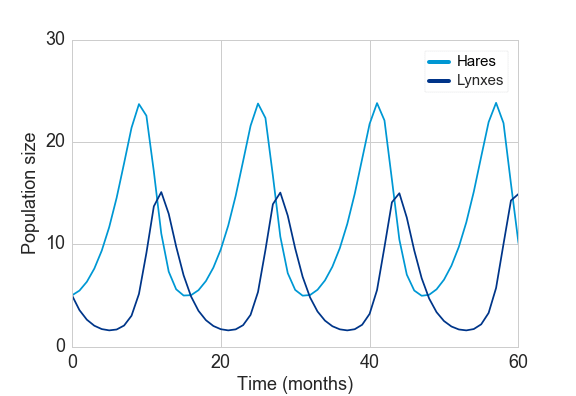
\includegraphics[scale=0.6]{lotka}
		\caption{Esempio di soluzione numerica di equazioni di Lotka-Volterra}
	\end{figure}
	
	Ovviamente il numero esatto di prede e predatori non seguirà esattamente questo andamento ma ci oscillerà intorno, specialmente nel caso di un campione piccolo.
	Bisogna quindi introdurre una densità di probabilità nell'avere $x$ prede e $y$ predatori:
	\[P\arg{x,y,t}\]
	Dopo un tempo $\d t$, le probabilità che la popolazione sia cambiata (la si fa cambiare di una unità perchè il cambio di due unità è di ordine $\d t^2$) sono:
	\[p_{x\rightarrow x+1}=a\,x \d t	\]
	\[p_{(x,y)\rightarrow (x-1,y+1)}=b\,xy\d t\]
	
	\[p_{y\rightarrow y-1}=c\,y\d t\]
La probabilità che resti uguale è quindi:

\[p_{(x,y)\rightarrow (x,y)}=1-(a\,x+b\,xy+c\,y)\d t\]
Questo genere di equazioni, che descrivono singole transizioni, prendono il nome di \textbf{birth death master equations}.

	Le equazioni precedenti si riscrivono:
	\[P\arg{x,y,t+\d t}=\tdv P\arg{x,y,t} \d t+P\arg{x,y,t}=\]\[= a (x-1) P\arg{x-1,y,t}\d t+b\, (x+1)(y-1) P\arg{x+1,y-1,t}\d t+c\,(y+1)P\arg{x,y+1,t}\d t+P\arg{x,y,t} [1-(ax+b(xy)+cy)]\d t	\]	\boxedeq{Volterra}{\tdv P\arg{x,y,t} = a (x-1) P\arg{x-1,y,t}+b\, (x+1)(y-1) P\arg{x+1,y-1,t}+c\,(y+1)P\arg{x,y+1,t}-P\arg{x,y,t} (ax+b(xy)+cy)}
	C'è una importante precisazione da fare su questo risultato: abbiamo mandato $\d t $ a 0 per poter approssimare con una derivata la $P$; questo si riduce a dire che la popolazione di un istante successivo dipende solo dalla popolazione l'istante precedente, così come la posizione nel moto browniano dopo un istante dipende dalla densità di probabilità nell'istante precedente.		\\
	Il punto è che, in biologia, possono esserci correlazioni 
	su tempi anche piuttosto lunghi, ad esempio ereditarietà di comportamenti o caratteristiche genetiche.\\
	Rispetto all'equazione di Langevin, che descrive una traiettoria deterministica ma dovuta ad una forza casuale (è come dire che si segue una delle possibili evoluzioni del sistema), si sta risolvendo, in questo caso, un'equazione differenziale che calcola l'effettiva distribuzione di probabilità, e non solo un sample dell'intero ensemble (come è il caso di Langevin).\\ Le fluttuazioni in questo tipo di modello sono grosso modo dell'ordine di $\sqrt{n}$, con $n$ numero di individui (è naturale se si pensa che sono modelli tipo random-walk)
	
	\section{Rumore Shot}
	Questo rumore è dovuto alla natura discreta della carica elettrica.
	Supponiamo di misurare il segnale ai capi di una certa resistenza, per un tervallo di tempo  di misura $T_m$.
	Se nella resistenza scorre una corrente $I$, vuol dire che dalla resistenza è uscita una carica $Q=I\,T_m=N q$ dove $q$ è la carica dell'elettrone ed $N$ è il numero di elettroni che sono usciti dalla resistenza.\\	L'importante assunzione da fare per continuare la trattazione è che gli elettroni siano indipendenti gli uni dagli altri, ovvero in un tempo di osservazione $T_m$ la distribuzione degli elettroni è uniforme; questo può non essere vero per grosse correnti, quando si iniza ad accumulare della carica che impedisce il passaggio di altri elettroni contemporaneamente.
	\\Sia $n$, il numero di elettroni passati dopo un tempo $t$, la nostra variabile casuale. Assumendo una corrente $I$, si ha che la probabilità che passi un elettrone in un tempo $\d t$ è \[\d p=\f{I}{q} \d t\]
	Si possono scrivere delle equazioni \textbf{birth-death} per n:
	\[\text{Prob}_{n\rightarrow n+1}=\f{I}{q} \d t\]
	Quindi, introducendo una distribuzione di probabilità per $n$:
	\[P\arg{n,t+\d t}=P\arg{n,t}(1-\f{I}{q} \d t)+P\arg{n-1,t}\f{I}{q} \d t\]
	Da cui si fa la solita approssimazione al prim'ordine:
	\[\tdv P=\left(P\arg{n-1,t}-P\arg{n,t}\right)\f{I}{q} 	\]
	Per risolvere questo tipo di equazioni, dove l'altro argomento, oltre a $t$ è un indice discreto (che comincia da 0), si introduce la cosiddetta \textbf{funzione generatrice} $G$.
	\[G\arg{s,t}=\sum_{n=0}^\infty s^n P\arg{n,t}\]

	\[\tdv G=\sum_n s^n \tdv P=	\f{I}{q}\sum_n s^n \left(P\arg{n-1,t}-P\arg{n,t}\right)=	\]
	\[=\f{I}{q}\sum_n s^n P\arg{n-1,t}-\sum_n s^nP\arg{n,t}=\f{I}{q}\sum_n s\,s^{n-1} P\arg{n-1,t}-\sum_n s^nP\arg{n,t}=\]
	Nella prima sommatoria posso cambiare indice da $n-1$  ad $n$ (visto che comunque il primo termine, con $n=0\implies n-1=-1$ era nullo perchè $P\arg{-1,t}=0$):
	\[=\f{I}{q}\sum_n s^{n}\left( s\,P\arg{n,t}- P\arg{n,t}\right)=\f{I}{q}(s-1) G\arg{s,t}\]
	Adesso ci siamo ridotti ad un'equazione differenziale:
	\[\tdv G=(s-1)\f{I}{q}G			\]
	\[G=A\,\exp({ \f{I(s-1)}{q}t})\]
	A $t=0$, $n=0\implies G=1\implies A=1$.\\
	Ritornando alla $P$
	\[G=\sum_n \exp(-\f{I}{q}t) \left(\f{I}{q}t\right)^n\f{s^n}{n!}			\]
	\[P=\exp(-\f{I}{q}t) \left(\f{I}{q}t\right)^n\f{1}{n!}	\]
	Ovvero la $P$ è in ogni istante un Poissoniana con media di elettroni accumulati $N=\f{I}{q}t$.\\
	Vogliamo trovare un'espressione per la corrente $I\arg{t}$. Sia $N\arg{t}$ la variabile casuale che conta il numero di elettroni misurati in ogni istante.
	\\Questa quantità è discontinua, nel senso che ad ogni passaggio di elettrone aumenta di uno come un gradino; di conseguenza la sua derivata sarà una $\delta$.
	\[\mu\arg{t}=\dv{N}{t}=\sum_k \delta\arg{t-t_k}\]
Dove i $t_k$ sono i tempi di passaggio dei vari elettroni.
Mentre passa un elettrone, la corrente misurata si estende per un certo tempo  $\tau$, in particolare si può introdurre la corrente generata da un singolo elettrone $F$ che passa all'istante 0:
		\[\int_{t=0}^{+\infty} F\d t =q			\]
		Dove $q$ è la carica dell'elettrone.
		In questo modo la corrente è, considerando che all'istante $t'$ passano $\mu \d t'$ elettroni:
		\[I\arg{t}=\int F\arg{t-t'} \mu\arg{t'} \d t'			\]
		Ad esempio si può prendere \[F=q\alpha e^{-\alpha t}\Theta\arg{t}\]
		
		Dove $\Theta$ è la funzione a gradino.\\
		Derivando l'espressione precedente:
		\begin{equation}
\dv{I}{t}=\int \dv{F\arg{t-t'}}{t} \mu\arg{t'} \d t'	=\int(-\alpha F\arg{t-t'}+\delta\arg{t-t'} \alpha q) \mu\arg{t'} \d t'	=-\alpha I	+\mu \alpha q	
\label{eq1}
	\end{equation}
		Al momento, $\mu$ è ancora una variabile casuale.
	

		Usando l'approccio di Langevin, e mediando ambo i membri:

\[\dv{\ave{I}}{t}=-\alpha \ave{I}	+\ave{\mu}	\alpha q\]
La corrente stazionaria misurata si trova imponendo la derivata $=0$:
	\[\ave{I}=I\arg{+\infty}=q\ave{\mu}	\]
	Dove $\ave{\mu}$ è il numero medio di elettroni al secondo.\\
	Vogliamo trovare la varianza della corrente.\\
È ora conveniente usare una variabile a media nulla, quindi definisco:
\begin{equation}
	\d \eta=\left(\mu-\ave{\mu}	\right) \d t
	\label{eta}
\end{equation}
Che ha il significato di oscillazione di numero di elettroni raccolti in un tempo $\d t$.
Moltiplicando l'equazione differenziale per $I \d t$ :
\begin{equation}
I \d I=-\alpha {I^2} \d t+\alpha q {\mu I}\d t	\label{eq2}
\end{equation}
A questo punto c'è una sottigliezza notevole: si vorrebbe scrivere $\d (I^2)= 2 I\d I$, ma questa formula è \textbf{sbagliata} per I variabile casuale. Il problema sta nel fatto che il termine $(\d I)^2$ che di base sarebbe al second'ordine, in realtà è al prim'ordine in $\d t$. Questo perchè $\d \eta=\d N-\ave{\mu} \d t$ è una variabile Poissoniana, così come $\d N$.\\
Facendo la varianza e ricordando che $\ave{\d \eta}=0$, e che $\d N$ è una variabile Poissoniana (varianza=valor medio):
\[\Var{(\d \eta)}=\ave{(\d \eta)^2}=\Var(\d N)=\ave{\d N}=\ave{\mu}	\d t	\] 
Quindi si vede che la media di $(\d \eta)^2$ è al prim'ordine in $\d t$ (questa proprietà orribile viene dal fatto che le funzioni a gradino come $N$ sono...poco regolari).
Ora vogliamo controllare se il valor medio di $(\d I)^2$ è al prim'ordine in $t$. Moltiplicando l'espressione \ref{eq1} per $\d t$ e usando la definizione \ref{eta}:
\[{\d I}=-\alpha I	\d t+\mu \alpha q \d t=-\alpha I	\d t+\ave{\mu} \alpha q \d t	+\d \eta \alpha q 
\]
\[({\d I})^2=(-\alpha I	\d t+\ave{\mu} \alpha q \d t+\d \eta \alpha q)^2	\]
Quando facciamo il quadrato l'unico termine al prim'ordine in $\d t$ è $(\d \eta)^2$ perchè il pezzo $\ave{\mu} \alpha q \d t$ è una costante (quindi un pezzo super-regolare) moltiplicato per $\d t$ (quindi certamente al second'ordine in $\d t$) e il pezzo $I\d t$ è un'integrazione nel tempo di $\d I$ e quindi è certamente più regolare di questo rispetto alla variabile $t$. Dato che noi stiamo guardando la regolarità di $\d I$, questo pezzo sicuramente non può contribuire.
Quindi:
\[\ave{(\d I)^2}=\alpha\left(	 q\right)^2	\ave{\mu} \d t	\]
Ora abbiamo tutti gli ingredienti per la varianza di $I$:
\[\ave{\d(I)^2}=\ave{\left(I+\d I\right)^2 -I^2}=\ave{(\d I)^2}+2\ave{\,I \d I	}=\left(	\alpha q\right)^2	\ave{\mu} \d t+2\ave{I \d I}	\]
Inserendo in \ref{eq2}:

\[ \f{1}{2}\d (I)^2=-\alpha {I^2} \d t+\alpha q {\mu I}\d t+\f{1}{2}(\d I)^2	\]
Facendo la media e notando che $\mu$ ed $I$ sono scorrelate ($\mu$ indica l'arrivo di un elettrone, che è scorrelato dalla corrente dovuta agli elettroni che stavano prima)
\[\f{1}{2} \d \ave{I^2}=-\alpha \ave{I^2} \d t+\alpha q \ave{\mu I}\d t+\f{1}{2}\ave{(\d I)^2}=-\alpha \ave{I^2} \d t+\alpha q \ave{\mu} \ave{I}\d t	+\f{1}{2}\left(	\alpha q\right)^2	\ave{\mu} \d t\]
Imponendo $ \d \ave{I^2}=0$ per andare a guardare il valore stazionario della varianza (ovvero il suo valore per $t\rightarrow+\infty$ )si ha:
\[-\alpha \ave{I^2} +\alpha q \ave{\mu} \ave{I}	+\f{1}{2}\left(	\alpha q\right)^2	\ave{\mu} =0\implies \ave{I^2} = q^2 \ave{\mu} ^2	+\f{1}{2}\alpha	 q^2	\ave{\mu} \]
\[\Var(I)=\ave{I^2}-\ave{I}^2=\ave{I^2}-q^2\ave{\mu}^2=\f{1}{2}\alpha	 q^2	\ave{\mu}=\f{1}{2}{\alpha}{q}	\ave{I}\]
\boxedeq{shot1}{\Var(I)=\f{1}{2}{\alpha}{q}	\ave{I}}
Nella trattazione solita del rumore shot, si considera un tempo di misura finito e l'errore dovuto alla varianza degli elettroni raccolti va a $0$ su tempi infiniti. Qui, invece, l'errore trovato è quello a cui tende il sistema in un tempo infinito, ed è dovuto non ad errori sui conteggi (che può essere ammazzato con tempi di campionamento maggiori), ma al fatto che la corrente arriva in pacchetti distinti. \\Tanto più sono distinti questi pacchetti (ovvero un elettrone porta una $\delta$ di corrente), tanto più è grossa la varianza.
\\Infatti, nel limite $\alpha\rightarrow\infty$ la corrente di singolo elettrone $F$ tende ad una delta di Dirac e la varianza calcolata diverge.
\subsection{Errore sui conteggi}
Come accennato, se campioniamo la corrente in un tempo finito $T_m$ compare un altro errore dovuto all'incertezza di elettroni raccolti.\\ Detta $N$ la variabile casuale Poissoniana di elettroni raccolti nel tempo di misura, e considerando una corrente media $I=\f{N \,q}{T_m}$:
\[I=\f{N q}{T_m}\implies\Var (I)=\Var(N)\left(\f{q}{T_m}\right)^2=N\left(\f{q}{T_m}\right)^2=I\left(\f{q}{T_m}\right)	\]
Questo errore però va a $0$ su tempi molto grandi. Come l'errore trovato in precedenza, anche questo è un effetto della discretizzazione della carica (mandando $q\rightarrow0$ entrambi gli errori vanno a 0).


\section{Processi di Markov}
Immaginiamo di avere una certa variabile $X\arg{t}$ dipendente dal tempo. Misurandola ai tempi $t_1,t_2,\ldots$ si avrà una certa distribuzione di probabilità per le varie misure:
\[p\argg{x_1,t_1;x_2,t_2;x_3,t_3;\ldots}		\]
Supponendo invece di \textbf{aver misurato } la variabile ai tempi $\tau_1,\tau_2,\ldots$, si altererà la distribuzione di probabilità per le misure successive: bisognerà parlare di probabilità condizionata:
\[p\argg{x_1,t_1;x_2,t_2;x_3,t_3;\ldots|y_1,\tau_1;y_2,\tau_2;y_3,\tau_3}	\]
\begin{defn}[Processo di Markov]
	Si parlerà di processo di Markov se di una serie di misure, la probabilità condizionata sarà influenzata solo dall'ultima misura compiuta, ovvero se:
\[p\argg{x_1,t_1;x_2,t_2;x_3,t_3;\ldots|y_1,\tau_1;y_2,\tau_2;y_3,\tau_3;\ldots}=p\argg{x_1,t_1;x_2,t_2;x_3,t_3;\ldots|y_1,\tau_1}\]
Con $\tau_1\ge\tau_2\ge\tau_3\ldots$
\end{defn}
Usando la proprietà \ref{abuso1}:
\[p\argg{x_1,t_1}=\int p\argg{x_1,t_1;x_2,t_2}\d x_2=	\int p\argg{x_1,t_1|x_2,t_2}p\argg{x_2,t_2}\d x_2\]
Ora invece supponiamo di avere a che fare con un processo di Markov. Riscrivo l'equazione precedente, solo aggiungendo l'ipotesi di aver fatto la misura $x_3$ al tempo $t_3\le t_2\le t_1$ (quindi mi basterà aggiungere questa condizione):
\[p\argg{x_1,t_1|x_3,t_3}=	\int p\argg{x_1,t_1|x_2,t_2;x_3,t_3}p\argg{x_2,t_2|x_3,t_3}\d x_2\]
ma ora, usando l'assunzione di Markov:
	\[p\argg{x_1,t_1|x_2,t_2;x_3,t_3}=p\argg{x_1,t_1|x_2,t_2}\]
Sostituendo si ottiene l'equazione di Chapman-Kolmogorov:
\boxedeq{Chapman}{p\argg{x_1,t_1|x_3,t_3}=	\int p\argg{x_1,t_1|x_2,t_2}p\argg{x_2,t_2|x_3,t_3}\d x_2}

\begin{defn}[Processi stazionari]
	Un processo con misure a vari tempi, come quelli descritti prima, è detto \textbf{stazionario} se è invariante per traslazioni temporali globali

\[p\argg{x_1,t_1;x_2,t_2;x_3,t_3;\ldots}=
p\argg{x_1,t_1+\tau;x_2,t_2+\tau;x_3,t_3+\tau;\ldots}		\]
\end{defn}
\subsection{Continuità nei processi di Markov}
Supponiamo di avere una distribuzione $p(x,t|y,\tau)$ che descriva un processo di Markov: sotto quali ipotesi ci si aspetta che sia continua (nel dominio delle $t$), ovvero che non ci siano salti?\\
Fare un salto vuol dire che in ogni istante di tempo (ovvero in ogni intervallino $[t,t+\d t]$) c'è una probabilità infinitesima di fare un salto di una quantità non infinitesima, ad esempio
\[p_{\text{salto nell'intervallo} [t,t+\d t]}=\lambda	\d t	\]
Un processo di questo tipo porta ad una distribuzione esponenziale se $\lambda$ è una costante;infatti la probabilità di non aver ancora fatto salti al tempo $t$ è la probabilità di non fare un salto in un intervallino ampio $\d t$ elevata al numero di intervallini:
\[p_\text{no salti al tempo t}=\left(1-\lambda\d t\right)^{\f{t}{\d t}}=e^{-\lambda t}			\]
Se invece la probabilità fosse del tipo
\[\d p=\lambda(\d t)^2		\]
chiaramente non si potrebbero avere salti (il limite precedente farebbe sempre $1$)\\
Quindi, la nostra richiesta per la continuità è che 
\boxedeq{ContinuityM}{\forall\epsilon>0\:\:	\lim_{\d t\rightarrow0}	\f{p(x+\epsilon,t+\d t|x,t)}{\d t}=0		}
ovvero che la probabilità di avere un salto finito $\epsilon$ in un intervallino ampio $\d t$ vada a 0 più forte di $\d t$.
\begin{exmp}[processo di Cauchy]
	È un esempio di processo non continuo:
	\[p\argg{x,t+\Delta t|x_0,t}=\f{1}{\pi}\f{\Delta t}{(x-x_0)^2+(\Delta t)^2}		\]
	In questo caso la probabilità di fare un salto ampio $y$ al secondo è $\f{1}{\pi\left(y^2+(\d t)^2\right)}\d y$
	
\end{exmp}
\begin{exmp}[Diffusione]
Utilizzando l'equazione \ref{Diffusion}, si vede che la probabilità di fare un salto va a 0 come:
\[\sim\f{1}{\sqrt{\d t}}e^{-\f{A}{\d t }}\]
Quindi più forte di qualsiasi potenza. Questo assicura la continuità ma \textbf{non} la differenziabilità (che infatti non c'è)
\end{exmp}
\subsection{Equazione differenziale di Chapman-Kolmogorov}
Per ridurre l'equazione \ref{Chapman} ad un'equazione differenziale, devono esistere i seguenti tre limiti: il primo ha a che fare con i salti discontinui, le altre due sono collegate con moti continui:\label{bbboh}
\begin{enumerate}
		\item \[	\lim_{\d t\rightarrow0}	\f{p(\pos,t+\d t|\vec{z},t)}{\d t}=W(\pos|\vec{z},t)\]
	\item  Questo prende il nome di \textbf{vettore di Drift}
	 \[	\lim_{\d t\rightarrow0}\f{1}{\d t}\int_{|\pos-\vec{z}|<\epsilon}(x_i-z_i){p(\pos,t+\d t|\vec{z},t)}   \d^n \pos=A_i(\vec{z},t)+O\arg{\epsilon}\]	
	 
	 
	 \item Questa è detta \textbf{Matrice di diffusione}
	 \[	\lim_{\d t\rightarrow0}\f{1}{\d t}\int_{|\pos-\vec{z}|<\epsilon}(x_i-z_i)(x_j-z_j){p(\pos,t+\d t|\vec{z},t)}   \d^n \pos=B_{ij}(\vec{z},t)+O\arg{\epsilon}\]
	
	
	
	
	
	
	
	
	
	
	

\end{enumerate}

Inolte tutti i limiti successivi di questo tipo devono essere zero: sia $n_i$ un vettore qualunque di norma unitaria:

\[|C_{ijk} n_in_jn_k|=\lim_{\d t\rightarrow0}\f{1}{\d t}|\int_{|\pos-\vec{z}|<\epsilon} (x_i-z_i)n_i\left[\vec{n}(\pos-\vec{z})\right]^2{p(\pos,t+\d t|\vec{z},t)} |  \d^n\pos\le\]\[\le\lim_{\d t\rightarrow0}\f{1}{\d t}\int_{|\pos-\vec{z}|<\epsilon} |(x_i-z_i)n_i|\left[\vec{n}(\pos-\vec{z})\right]^2{p(\pos,t+\d t|\vec{z},t)}   \d^n	\pos\le\]\[\le\lim_{\d t\rightarrow0}\f{1}{\d t}\int_{|\pos-\vec{z}|<\epsilon} \epsilon\cdot 1 \,(x_j-z_j)(x_k-z_k)n_kn_k{p(\pos,t+\d t|\vec{z},t)}   \d^n\pos=B_{jk}n_jn_k \epsilon=O\arg{\epsilon}\]
Il motivo per cui questa dimostrazione non funziona per dimostrare che $B$ è $\sim\epsilon A$ è che l'argomento dell'integrale di $A$ non è sempre positivo e quindi non posso portare dentro il valore assoluto (mentre posso farlo con $B$ visto che è quadratico l'argomento).
\\La prima proprietà indica il rate di salto di ampiezza finita per secondo. Se $W$ è continua, questo rate deve essere $0$ (per $x\ne z$). Infatti, la probabilità di fare un salto finito ampio almeno $\epsilon$ per un intervallo $T$ è:
\[\int_{t=0}^{T}\int_{|\pos-\vec{z}|\ge\epsilon}		{p(\pos,t+\d t|\vec{z},t)}\d^n\pos=\int_{t=0}^T\int_{|\pos-\vec{z}|\ge\epsilon}	W(\pos|\vec{z},t) \d t\d^n\pos\]	
Se questo integrale è nullo per ogni $\epsilon$, vuol dire che non si possono fare salti finiti e che quindi $W$ è nella per $\pos\ne\vec{z}$.\\			
L'equazione differenziale che si ricava è la seguente (la derivazione è un po' pesante e non particolarmente illuminante, si usa una funzione test che poi si integra per parti)
\begin{multline}
\partial_t p(\vec{z},t|\vec{y},t')=\\=-\pdv{z_i}[A_i(\vec{z},t) p(\vec{z},t|\vec{y},t')]+\frac{1}{2}\pdv{}{z_i}{z_j}[B_{ij}(\vec{z},t)p(\vec{z},t|\vec{y},t')]+\int \d \pos [W(\vec{z}|\pos, t)p(\pos|\vec{y},t')-W(\vec{x}|\vec{z}, t)p(\vec{z},t|\vec{y},t')]\end{multline}
\subsection{Condizioni al contorno}
La più sensata da prendere è $p(\pos,t|\vec{y},t)=\delta(\pos-\vec{y})$, ovvero che la distribuzione di probabilità al tempo iniziale sia una $\delta$, visto che si conosce esattamente la posizione iniziale.\\Per gli esempi successivi si prende $t=0,\vec{y}=\pos_0$, quindi posso scrivere $p(\pos,t)$ tenendo in mente queste condizioni al contorno.
\\Riguardo l'esistenza di una soluzione, ci sono varie condizioni. Una di queste è che la matrice $B_{ij}$ sia semidefinita positiva (e che esistano i vari limiti che definiscono $A,B,W$).\subsection{Backward equation}
Volendo si può anche considerare la seguente probabilità
\[p(\pos,0|\pos',t)\quad\quad t<0\]
Dove si considera, però $\pos$ fissa e si prendono $t,\pos'$ come variabili.\\Le condizioni al contorno sono sempre le stesse, visto che
\[p(\vec{z},t|\vec{y},t')=\delta(\vec{y}-\vec{z})\]
ma stavolta si risolve per $t'<t$.\\Con un processo analogo a quello che porta all'equazione differenziale di Chapman-Kolmogorovv, si ottiene:
\begin{equation}
{\pdv{p(\vec{z},t|\vec{y},t')}{t'}	=-A_{i}\pdv{p(\vec{z},t|\vec{y},t')}{{y}_i}-\f{1}{2}B_{ij}\pdv{p(\vec{z},t|\vec{y},t')}{y_i}{y_j}			
+\int \d \vec{x}\left( W(\vec{x}|\vec{y},t')p(\vec{z},t|\vec{y},t')-W(\vec{x}|\vec{y},t')p(\vec{z},t|\vec{x},t')\right)}\label{rev}
\end{equation}
Dato che l'evoluzione temporale è omogenea (le equazioni non dipendono esplicitamente dal tempo), $p$ dipende solo dalla differenza $t-t'$, quindi volendo si può scrivere l'equazione precedente derivando rispetto a $t$ e cambiando il segno della derivata.
\\In realtà c'è un trucco molto semplice per ricavare questa equazione:
sia $t>t'>t''$, allora
\[\pdv{p(\kvec,t|\vec{y},t'')}{t'}=0=\pdv{t'}\int 	 p(\kvec,t|\vec{z},t')p(\vec{z},t'|\vec{y},t'')\d \vec{z}=\int 	\left\{ \pdv{p(\kvec,t|\vec{z},t')}{t'}p(\vec{z},t'|\vec{y},t'')+{p(\kvec,t|\vec{z},t')}\pdv{p(\vec{z},t'|\vec{y},t'')}{t'}\right\}\d \vec{z}=	\]
Per brevità delle formule ometto il pezzo con $W$, ma è chiara la generalizzazione:
\[=\int 	\left\{ \pdv{p(\kvec,t|\vec{z},t')}{t'}p(\vec{z},t'|\vec{y},t'')+{p(\kvec,t|\vec{z},t')}\left(-\pdv{z_i}[A_i(\vec{z},t') p(\vec{z},t'|\vec{y},t'')]+\frac{1}{2}\pdv{}{z_i}{z_j}[B_{ij}(\vec{z},t')p(\vec{z},t'|\vec{y},t'')]\right)\right\}\d \vec{z}=	\]
Integrando per parti il secondo addendo si spostano tutte le derivate spaziali su $p(\kvec,t|\vec{z},t')$. Raccogliendo il fattore $p(\vec{z},t'|\vec{y},t'')$ nei due addendi si ha alla fine un'equazione del tipo
\[\int \d	\vec{z}p(\vec{z},t'|\vec{y},t'')\left(F(\kvec,t,\vec{z},t')\right)\]
Dove $F$ è la backward equation. Ma per l'arbitrarietà dell'estremo $t''$, che può essere fatto variare a piacere, si ha che $F=0$, cioè la backward equation.

\subsection{Esempi}
\subsubsection{Processi Jump}
È il caso in cui l'unico termine $\ne 0$ è $W(\pos,t)$. \\In questo caso i cammini di prova tipici sono costanti a tratti (perchè c'è una probabilità finita di restare nell'origine, grazie al fatto che non si sta derivando la $\delta$) e compie salti random con un'ampiezza determinata dalla distribuzione di $W$.
\\ Per $\Delta t$ piccoli, si può scrivere, al prim'ordine
\[p(\pos,t+\Delta t)=\delta(\pos-\pos_0)\left(1-\Delta t \int \d \vec{z} W(\vec{z},t|\pos_0)		\right)+W(\pos,t|\pos_0)\]
Quindi un cammino nello spazio delle posizioni ha una certa probabilità per unità di tempo di saltare.
\subsubsection{Equazione di Fokker-Planck}
È il sottocaso più importante, e generale: consiste nel prendere $W=0$.\\Quindi stiamo descrivendo un processo continuo diffusivo, e la motivazione per questa affermazione è la seguente: supponiamo $A_i,B_{ij}$ circa costanti nel range di variazione \emph{spaziale} tipico della $p$ (ad esempio nei primi istanti del moto, quando la probabilità è fortemente piccata in una regione piccola) e costanti temporalmente ; questa approssimazione equivale a trascurare le derivate di vettore di drift e matrice di diffuzione.\\Si ottiene una equazione di diffusione!
\[\partial_tp=-A_i\partial_i p+B_{ij}	\partial^2_{ij}p	\]
Che ha come soluzione (sia $n$ il numero di dimensioni)
\[p(\pos,t|y=0,t=0)=\f{1}{\sqrt{(2\pi)^n \det(B)t}}\exp(-(x_i-A_it)B_{ij}(x_j-A_j t))\]
Cammini di prova sono continui ma non differenziabili (è noto che il moto browniano sia irregolare)
\subsubsection{Equazione di Neuville}
L'esempio più facile da fare è quello in cui $W,B_{ij}=0$ e c'è solo il termine con $A_i$.\\Questo termine, da solo, \textbf{descrive un moto deterministico}. Il motivo è che il termine rappresenta un drift uniforme della distribuzione, e non ne altera la forma.
\\Per dimostrarlo esplicitamente: prendo come guess per la soluzione\[p(\pos,t)=\delta(\pos-\vec{s}(t))\]
dove $\vec{s}(t)$ è una qualche funzione del tempo.
\[\partial_t p=-\dot{{s}}_i \partial_i(\delta(\pos-\vec{s}(t)))=-\pdv{}{x_i}[A_i(\pos,t)\delta(\pos-\vec{s})]=-\pdv{}{x_i}[A_i(\vec{s}(t),t)\delta(\pos-\vec{s})]=-A_i(\vec{s}(t),t)\pdv{}{x_i}[\delta(\pos-\vec{s})]\]
Che quindi è verificata se \[\dot{\vec{s}}=\vec{A}\]
Il significato intuitivo di $\vec{A}$, quindi, è quello di velocità istantanea di traslazione della distribuzione.
\subsubsection{Processi di Ornstein-Uhlenbeck}\label{boh}
Si tratta di un caso della Fokker-Planck 1-D, con $A=-kx$, $B=D=const$.\\
\[\pdv{p}{t}=\pdv{[kxp]}{x}+\f{1}{2}D\pdv[2]{p}{x}\]	
Cerco le soluzioni stazionarie:
\[\pdv{x}[kx+\f{1}{2}D\partial_xp]=0\implies kxp+\f{1}{2}D\partial_xp=const\]
\[\partial_x\ln (p)	=-kx^2+C	\]
Quindi $p$ è una gaussiana (la costante è fissata dalla normalizzazione)
\\In trasformata di Fourier nelle posizioni (uso $s$ come vettore d'onda), si ottiene	\[\tdv \phi+ks\partial_s\phi=-\f{D}{2}s^2	\phi\]
oppure, cambiando variabile $g=\ln(\phi)$
\[\pdv{g}{t}+ks\pdv{g}{s}=-\f{D}{2}s^2	\]

Per risolvere questa equazione, uso il \textbf{metodo delle caratteristiche}, descritto in \ref{nonhoidee}
\[\f{\d g }{-\f{D}{2}s^2g}=\f{\d s}{k s}		\]
\[u=g	+\f{D}{4k} s^2	\]
\[{\d t }=\f{\d s}{k s}\]
\[v=t-\f{1}{k}\ln(s)\]
La soluzione più generale si ha scrivendo (c'è un mucchio di arbitrarietà che sfrutto):\[e^{u}-f(e^{-kv})=0\]
\[\phi e^{\f{Ds^2}{4k}}=f(se^{kt})	\]
La soluzione generale è :
\[\phi=e^{-\f{Ds^2}{4k}}f(se^{-kt})\]
Bisogna imporre le condizioni al contorno, usando le solite, queste si traducono, in trasformata, in:\[\phi(s,t=0)=e^{-isx_0}\]
Da cui si trova che la soluzione è
\[\phi(s,t)=  \exp(-\f{Ds^2}{4k}+\f{Ds^2}{4k}e^{-2kt})\exp(-i s x_0e^{-kt})\]
che andrebbe antitrasformata.\\Visto che $\phi$ è l'esponenziale di un polinomio quadratico in $s$, la sua antitrasformata è sempre l'esponenziale di un polinomio quadratico (una \textbf{Gaussiana!}), con media (si vede dal termine di traslazione in trasformata $e^{-is \Delta x(t)}$):
\[E[{X(t)}]=x_0e^{-kt}\]
e varianza (è il doppio del coefficiente del termine quadratico in trasformata)
\[E[X^2]=\f{D}{2k}\left(1-e^{-2kt}\right)\]
Volendo studiare la correlazione del modello, ovvero
\[E[X(t+\tau)X(t)]\]
è conveniente farlo nel caso stazionario, ovvero nel lontano futuro $t\ra \infty$: in questo caso si può approssimare $p(x_1,t|x_0,t=0)$ con una gaussiana centrata nell'origine con varianza $\f{D}{k}$, e  $p(x_2,t+\tau|x_1,t)=p(x_2,\tau|x_1,0)$ (per invarianza sotto traslazioni temporali) con una gaussiana centrata in  $x_1 e^{-k\tau}$, quindi l'integrale in $x_2$ che è semplicemente il valor medio di $x_2$ restituisce $x_1e^{-k\tau}$ 
\[\int \d x_2\d x_1 x_2x_1	p(x_2,\tau|x_1,0)p(x_1,\infty|x_0,0)= \int \d x_1 x_1^2 e^{-k\tau}	e^{-\f{kx_1^2}{D}}	\f{1}{\sqrt{\f{D\pi}{k}}}=e^{-k\tau}\f{D}{2k}\]

Quindi decade esponenzialmente (normale, il sistema tende a restringersi)

\section{Random Walk 1-D}
Voglio studiare la random walk con un approccio di Master equation. Ci sono due tipi di Random Walk: 
\begin{enumerate}
\item Dopo un tempo $\tau$ fissato si salta in avanti o indietro (con probabilità uguale)
\[P(n,t+\tau)=\f{1}{2}	P(n-1,t)+\f{1}{2}	P(n+1,t)	\]
\item
Si ha una probabilità per unità di tempo $\mu$ di saltare	\label{due}
\[			P(n, t+\d t)= \mu P(n-1,t) \d t+\mu P(n+1,t)\d t- (1-2\mu\d t)P(n,t)\implies\]\[ \pdv{P}{t}=\mu \left(P(n-1,t)+ P(n+1,t)-2 P(n,t)\right)\]
\end{enumerate} Cambiando la scala temporale (in modo tale che $\tau$ sia molto piccolo), il primo tipo rientra nel secondo, perchè nell'intervallo di misura ci possono essere stati così tanti salti che di quanto si è spostata la particella è una variabile casuale.
\\Infatti, per $\tau $ infinitesimo:
\[P(n,t+\tau)\approx P(n,t)+\tau \pdv{P}{t}	=\f{1}{2}	P(n-1,t)+\f{1}{2}	P(n+1,t)	\]
Che è il caso 2 con $d=\f{1}{2\tau}$ (quindi $d$ grosso).\\
Queste distribuzioni si trovano con il metodo della funzione caratteristica (uso $e^{ins}$ perchè stavolta $n$ prende anche valori negativi):
\[G=\sum_{n=-\infty}^\infty  p(n,t)e^{-ins}\]
Moltiplicando il caso 2 per $e^{-ins}$ e sommando su $n$:
\[\pdv{G}{t}=-4\mu \sin^2(\f{s}{2})G\implies G=\exp\left(-4\mu t\sin ^2 \left(\f{s}{2}\right)			\right)		\]
Nell'ultimo passaggio si è utilizzata anche la condizione iniziale $p(n,t=0)=\delta_{n,0}$
\\
Nel caso 1, invece:
\[G_1(s, (N+1)\tau)=\cos(s)G_1(s,N \tau)			\]
\[G_1(s, N\tau)=\cos(s)^N\]

	\[G_1\ra \left(1+(-1+\cos(s))\right)^{\f{t}{\tau}}=	\left(1-{2}{}\sin^2\left(\f{s}{2}\right)\right)^{\f{t}{\tau}}		\]
Nel limite in cui anche $\tau\ra 0$, con $\f{s^2}{\tau}$ che resta finito (eqivale a dire che nelle $x$ si ha $\Delta x\propto \f{1}{s}\sim\f{1}{\sqrt{\tau}}$ ovvero la distribuzione è molto "broad", quindi con pochi salti non cambia forma):
\[G_1\ra \exp(-\sin(\f{s}{2})^2\f{2t}{\tau})		\]	
che è il caso 2 (sempre per $s$ piccolo) con $\mu=\f{1}{2\tau}$ (tutto ciò ha senso perchè s'è detto che limite caratteristica$\implies$ limite distribuzione).
\begin{obs}[Limite continuo]
Corrisponde a prendere la distribuzione delocalizzata in $n$, ovvero molto "broad". In trasformata, significa avere una distribuzione molto piccata nell'origine, con $s\approx 0$.\\L'alternativa , più chiara nei conti, è inserire una scala di lunghezza $l$ di spazio nel reticolo, in modo tale che $s\ra ls$ nella nuova scala (s non è più adimensionale). Mandare $l$ a 0 equivale a mandare il vecchio $s$ adimensionale a 0.
\\In ogni caso, il risultato è una distribuzione gaussiana nelle $s$

\[G\ra 	\exp(-{s^2\mu t}{})		\] 
con varianza ${2\mu t}$ (sempre ricordando che in trasformata $\phi\sim\exp(-\f{s^2\sigma^2}{2})$, o espandendo al second'ordine in $s$).\\
Il motivo per cui si ritrova il solito processo diffusivo (\textbf{Wiener process} è che, nella definizione \ref{due}), si può approssimare il pezzo tra parentesi con una derivata seconda:
\[\pdv[2]{P}{n}\approx2P(n)-P(n-1)-P(n+1)\]
riottenendo l'equazione di diffusione
\end{obs}
\section{Telegrafo random}
È un processo random con una variabile discreta che può prendere solo due valori, $a\econg b$, con probabilità di salto $\lambda,\mu$:
\\Volendo posso pensare la probabilità come un vettore $2D$:
\[p_0(t)=p(a,t)\quad \quad p_1(t)=p(b,t)\]

\[\pdv{\vec{p}(t)}{t}=\Op{M}\vec{p}\]
Con \[\Op{M}\begin{pmatrix}
-\lambda&\mu\\\lambda&-\mu
\end{pmatrix}\]
gli autovalori sono $0$ e $-\lambda-\mu$, e l'autovalore corrisponente a $0$ è la soluzione stazionaria, l'altra rilassa chiaramente con \[\exp(-[\lambda+\mu]t)\]
La soluzione stazionaria è (il prefattore serve a normalizzare)\[\vec{p}=\f{1}{\lambda+\mu}\begin{pmatrix}
\mu\\\lambda\end{pmatrix}\]
Da queste espressioni esplicite uno si può trovare tutto, ad es. varianza e correlazione. (la correlazione giustamente va già con l'esponenziale $e^{-(\mu+\lambda)t})$. La varianza che va giù esponenzialmente accomuna questo processo random a quello di Ohrnstein-Uhlenbeck, ed infatti viene utilizzato spesso come variante più semplice per modellizzare variabili random

\section{Analisi stocastica}
L'obiettivo è formalizzare l'approccio di Langevin per quanto riguarda differenziali di quantità random, dato che sembra molto semplice e potente da usare. \\L'approccio corretto è, più che scrivere equazioni differenziali (visto che le quantità non sono differenziabili), è quello di  utilizzare equazioni integrali.\\Il primo step è quindi scrivere  l'integrale di una quantità random.
\\ Si prende la quantità $\xi(t)$ rapidamente variabile e irregolare, che rispetta \[\ave{\xi}=0\]\[\ave{\xi(t')\xi(t)}=\delta(t-t')\] e si utilizza per fare i conti la variabile casuale $W$ ($W$ sta per Wiener)
\[\d W=\xi (t)\d t	\quad \quad W(t)=\int_0^t \xi(s)\d s	\]
Che descrive un processo di Markov, visto che
\[W(t)=\int^t_{t'} \xi(s)\d s+W(t')\]
Dipende solo da $W(t')$ e non da tempi precedenti.\\ 
Media e covarianza sono (suppondendo a $t=0$ di partire con $W=0$):
\[\ave{W}=0\]
 \[\ave{W(t)W(t')}=\ave{\int_0^t\int _0^{t'}	\xi(s)\xi(s')		} \d s \d s'=\int _0^t\int _0^{t'} \delta(s-s')\d s \d s'= \min(t,t')\]
Ora si può definire l'integrale:
si deve dividere l'intervallo di integrazione in $N$ punti $t_i\ge t_{i-1}$.\\ Siano inoltre $\tau_i\in [t_i,t_{i-1}]$
\\L'\textbf{integrale stocastico è definito come}:\[\int	 G(t)\d W(t)=\lim_{N\ra \infty} \sum_i G(\tau_i)[W(t_i)-W(t_{i-1})]				\]
	potendo prendere \[\tau_i=t_{i-1}+a(t_i-t_{i-1})\quad a\in [0,1]\]
il risultato dipende dalla scelta di $a$ (come si può mostrare facilmente prendendo $G=W$ 	).\\
Infatti, per $G=W$:
\[\ave{\int W(t)\d W}	=	\sum_i \ave{W(\tau_i)[W(t_i)-W(t_{i-1})]		}=\]
\begin{equation}
=\sum_i \tau_i-t_{i-1}=\sum_i a(t_i-t_{i-1})=a(t_N-t_0)	
\label{aint}
\end{equation}
che dipende da $a$.\\\textbf{L'integrale di Ito} corrisponde ad una scelta per $a$ di queste possibili definizione di integrali, ovvero 
\boxedeq{bb}{a=0}
Inoltre il limite $N\ra \infty$ è inteso come limite mean square \ref{ms}
\boxedeq{Stocint}{\int_{t_0}^{t_M}	 G(t)\d W(t)=\text{ms}-   \: \lim_{N\ra \infty} \sum_i G(t_{i-1})[W(t_i)-W(t_{i-1})]	}
\\ Per inciso, esistono altre scelte di $\alpha$, ad esempio $\alpha=\f{1}{2}$ è detto \textbf{integrale di Stratonovich}, ed è la scelta più intuitiva fisicamente da fare, mentre l'integrale alla ito viene usato per descrivere i \textbf{martingala} (Li uso dopo in \ref{Martina})
\\ \begin{defn}[Martingala]
È una sequenza di variabili casuali $x_i$ dove il valore di aspettazione di una variabile casuale è uguale al termine precedente della sequenza $E[x_i]=x_{i-1}$ 
\end{defn}
Il motivo per cui l'integrale di Ito $\int W\d W$ viene in media 0, è che si suppone l'incremento di $\d W$ indipendente dal valore di $W$ (è questo il significato fisico della scelta di $a$). Prendere $a=\f{1}{2}$ vuol dire prendere $W(t_i)$ come media del suo valore "vecchio" (nell'intervallo di tempo precedente) ed del suo valore nuovo dopo l'incremento. Quindi $W$ non è indipendente dal suo incremento ed il valor medio di $W\d W$ non è 0. 
\begin{defn}[Funzione non anticipante]
$G(t)$ è detta non anticipante se \emph{non} dipende dal valore dell'incremento di $W$ nel futuro, ovvero dalla quantità
\[W(s)-W(t)\quad	\forall s\ge t	\]
\end{defn}
\begin{exmp}[Funzioni non anticipanti]
Sono funzioni non anticipanti la $W(t)$ e tutte le funzioni $F(W(t))$ di questa quantità, chiaramente. \\Inoltre anche funzioni di $W(t')$ dove si prendono vari $t'$ precedenti a $t$; questa affermazione è compresa dalla generica quantità :
\[	\int^t_{0} F(W(t'))\d t' 	\]
(che comprende anche le quantità precedenti, a patto di usare delta di dirac come $F$)

\end{exmp}


\section{Integrali alla Ito}\label{ito}
Nella trattazione si userà sempre una $G(t)$ non-anticipante.\\La formula di Ito consiste sostanzialmente nel notare che $[\d W]^2=\d t$.
\\
Anzitutto voglio trovare  (suppongo $t\ge t'$)
\[\ave{\left(W(t')-W(t)\right)^2}=\ave{[\int_{t'}^t\xi (s) \d s]^2}=t-t'	\]
che traduce l'affermazione intuitiva di prima.
L'altro ingrediente che serve è
\[\ave{\left[\left(W(t')-W(t)\right)^2-(t-t')\right]^2}\]
Che si può trovare in modo analogo a prima, oppure notando che 
\[W(t')-W(t)=\int_{t'}^t \xi \d s	\]
è la somma di tante variabili casuali ($\xi(s)$) indipendenti. Quindi è una variabile gaussiana, con media nulla (perchè la media delle $\xi$ è 0). La varianza la si è calcolata prima
\[\ave{[\int_{t'}^t \xi \d s	]^2}=t-t'\]
E usando il fatto che, per una variabile gaussiana $\phi$ vale
\[\ave{(\phi^2-\sigma^2)^2}=2\sigma^4\]
Si trova \[\ave{\left[\left(W(t')-W(t)\right)^2-(t-t')\right]^2}=2\left(t-t'\right)^2\]
\\
La formula generale è
\[\int G(t) [\d W(t)]^2=\int G(t)\d t	\]
Dimostrarla equivale a far vedere che \[\text{ms}-\lim_{N\ra \infty} {\sum_i G(t_{i-1})[(W(t_i)-W(t_{i-1}))^2-(t_{i}-t_{i-1})]}=0		\] Cioè, ricordando la definizione del limite
\[\ave{\{\sum_i G(t_{i-1})[(W(t_i)-W(t_{i-1}))^2-(t_{i}-t_{i-1})]\}^2}=\]\[=
\ave{\sum_i G^2(t_{i-1})[\Delta W_i^2-\Delta t_i]^2}+2\sum_{i> j}\ave{G(t_{i-1})G(t_{j-1})	[\Delta W_j^2-\Delta t_j]^2[\Delta W_i^2-\Delta t_i]^2}	=\]
Il fatto che $G$ sia nonanticipante, ci dice che $\Delta W_i$ e $G(t_i)$ sono indipendenti, quindi ad esempio nel primo addendo, posso fare i valor medi separatamente dei due fattori, e sfruttare le formule date prima. Per il secondo addendo, l'ultimo fattore è indipendente dagli altri 3 per lo stesso motivo, ma il suo valore di aspettazione è 0, quindi annulla tutto l'addendo

\[=2\sum_i\ave{ G^2(t_{i-1})}(\Delta t_i)^2 \]

Ma questa quantità, se $G$ non fa troppo schifo, (ad esempio è limitata da una costante $A$) è 0, perchè $(\Delta t_i)^2$ è un differenziale (di una quantità NON stocastica) al quadrato. Esplicitamente, con $N$ divisioni dell'intervallo $T$:
\[\Delta t \sim\f{T}{N}\implies \sum_i \left(\Delta t_i\right)^2\sim N \f{T^2}{N^2}\quad \lim_{N\ra \infty}\sum_i \left(\Delta t_i\right)^2=0	\] 
Quindi si è mostrata la seguente formula per \textbf{integrali alla Ito}
\boxedeq{itomain}{\int G(t) [\d W(t)]^2=\int G(t)\d t}
Per inciso, i differenziali di ordine successivo $[\d W]^{2+N}$, sono tutti di ordine trascurabile nell'integrale.\\ Questo mostra anche la scelta di $a=0$ nell'integrale di Ito, che serve per l'indipendenza della $G(t)$ dal differenziale che la moltiplica; la formula infatti non vale per l'integrale di Stratonovich.\subsection{Formula di Ito}
Quando si fa il differenziale di una funzione 
\[\d f(W,t) 		\]
bisogna stare attenti agli ordini che si tengono. In particolare, bisogna mantenere il second'ordine in $W$ (la regola generale è pensare $\d W$ di ordine $\f{1}{2}$). 
\[\d f=\pdv{f}{t}\d t+\pdv{f}{W}\d W+\f{1}{2}\pdv[2]{f}{W} [\d W]^2		\]
Ma il differenziale $[\d W]^2$ converge con probabilità uno a $\d t$, quindi si ottiene la cosiddetta \textbf{formula di Ito}(sostituisco $\d t$)
\[\d f(W,t)=\left[\pdv{f}{t}+\f{1}{2}\pdv[2]{f}{W}\right]\d t+\pdv{f}{W}\d W\]
\begin{exmp} [cambio di variabile]
Se invece si ha una variabile casuale generica, del tipo
\[\d x	=A\d t+ B\d W	\]
e si vuole cambiare variabile, passando a $f(x,t)$, allora il nuovo differenziale  è
\[\d f=\pdv{f}{t}\d t+\pdv{f}\d x+\f{1}{2}\pdv[2]{f}{x}(\d x)^2=\left(\pdv{f}{t}+\f{1}{2}\pdv[2]{f}{x} B^2\right)\d t+\pdv{f}{x} A \d W		\]

\end{exmp}
\begin{exmp}["Esempio Importante"]
Come esempio, guardo il seguente integrale (che si era usato come esempio per mostrare come tipi diversi di integrazione portano risultati diversi)
\[\int_{t_0}^t 	W \d W=\f{1}{2}\left[\int \d W^2-(\d W)^2\right]=\f{1}{2}\left(W^2(t)- W^2(0)-(t-t_0)\right)			\]
Che, prendendo il valor medio (ricordando che $\ave{\Delta W^2}=\Delta t$), coincide con il valore per $a=0$ in \ref{aint}, cioè 0. L'integrale alla Stratonovich elimina l'ultimo addendo ( per integrali alla stratonovich valgono le solite regole del calcolo differenziale ).
\end{exmp}
\section{Stochastic Differential Equation (SDE)}
In generale, uno si tova ad integrare una roba di questo tipo
\[\d x= f(x)\d s+g(x) \d W		\]
Il problema di questa equazione è che, per colpa di $\d W$, $x$ è essa stessa una variabile stocastica, quindi anche $g(x)$ conterrà dei termini in $W$ stocastici, ad esempio.
\\ Per capire che una soluzione esiste ed è unica, almeno per scelte di $f$ e $g$ abbastanza regolari (ad esempio limitate e continue), l'ideale è pensare come integrare l'equazione numericamente.
\\L'idea è di andare a piccoli step, con incrementi $\d s$ deterministici, mentre si prende $\d W$ come una variabile casuale a media nulla e varianza $\d s$. In particolare, quello che si fa è  prendere $\d W$ con varianza $1$ e moltiplicarla per $\sqrt{\d t}$.
Il teorema del limite centrale assicura che i vari incrementi di $\d W$, se sono abbastanza densi, alla fine possono essere presi gaussiani, se uno va a guardare una scala di tempi $\Delta t\gg \d t$ (quindi è conveniente prenderli gaussiani dall'inizio).
\\Per una soluzione "analitica", si può andare di approssimazioni successive dell'equazione integrale associata
\[x^{n+1}(t)=\int_0^t	f(x^n(s))	\d s+g(x^n(s))\d W		\]
\[x^0(t)=x_0\]
\[x^1(t)=\int f(x_0,t)\d t+g(x_0,t) \d W=F(x_0,t)+g(x_0,t) W(t)		\]
\[x^2(t)\approx		\int f(x_0,t)\d t+{\pdv{f}{x}}	(x^1-x^0)\d t+g(x_0,t) \int \d W+\int {\pdv{g}{x}}(F(x_0,t)+g(x_0,t) W(t)-x_0	) \d W			\]
Quindi si vede che compaiono integrali del tipo $\int W \d W$, che possono essere risolti nei vari tipi di integrazione (Ito, Stratonovich, $\ldots$).	
\subsection{Legame con la Fokker Planck}
L'approccio del calcolo differenziale stocastico è completamente equivalente al campionamento di una variabile casuale con una distribuzione $p(x,t)$ che rispetta una certa equazione di Fokker-Plank; per dimostrarlo, si consideri $x$ variabile casuale
\[\d x =a (x,t) \d t +b(x,t) \d W		\]
Si vuole mostrare che $x$ è uguale, (nel senso stocastico \ref{distr}) ad una distribuzione di probabilità che rispetta la Fokker planck; quindi bisogna prendere una funzione $f(x)$ generica e valutarne il valor medio:
\[\ave{\dv{f(x(t))}{t}}=\f{1}{\d t} \ave{\d f}=\f{1}{\d t} \ave{\pdv{f}{x} \d x+\f{1}{2}\pdv[2]{f}{x} [\d x		]^2}			={\f{1}{\d t}} \left({\pdv{f}{x} a\d t+\f{1}{2}\pdv[2]{f}{x}	b^2 \d t	}		\right)=a\pdv{f}{x} + b^2\f{1}{2}\pdv[2]{f}{x}			\]
Per $\pdv{f}{x}$ si intende chiaramente $\ave{\pdv{f}{x}}$, si è usato che l'incremento di $x$ è scorrelato dal valore di $x$ in cui si calcola la derivata (cosa vera per SDE alla Ito, questo procedimento non vale, ad esempio, per SDE alla stratonovich).\\ In generale $x$ avrà una distribuzione di variabile casuale $p(x,t)$, quindi
\[\ave{a\pdv{f}{x} + b^2\f{1}{2}\pdv[2]{f}{x}}=\int 	\left(a\pdv{f}{x} + b^2\f{1}{2}\pdv[2]{f}{x}	\right)p(x,t)	\d x=\int	\left(-f\pdv{[a p(x,t)]}{x} + f\f{1}{2}\pdv[2]{[b^2 p(x,t)]}{x}		\right)\d x	\]
L'ultimo passaggio è un'integrazione per party, che \emph{corrisponde al valore per la derivata di x dato dall'equazione di Fokker Planck!}
\\È tutto più chiaro scrivendo
\[\ave{\dv{f}{t}}=\dv{t}[\int f(x) p(x,t)		]\d x	=	\int f \tdv p(x,t)		\d x	\]
e a questo punto si sostituisce $p$ dall'equazione di Fokker-Planck con $a=A$, $b^2=B$
\boxedeq{ITO-FP}{\d x =a (x,t) \d t +b(x,t) \d W	\ifandonlyif 	\tdv p(x,t)	=-\pdv{a(x,t)p}{t}+\f{1}{2}\pdv[2]{b(x,t)p}{x}
}
Si sottintende che la variabile $x$ è definita tramite un'integrazione alla Ito, altrimenti la formula di Ito usata nella derivazione non è valida.


\section{SDE alla Stratonovich}
Si indica con $\sint$ l'integrale alla Stratonovich.
In particolare, si valuta un integrale del tipo $\sint G(W(t),t) \d W$ con \[\sint G(W(t),t) \d W\equiv \text{ms}\lim_{N\ra \infty}\sum_i G(W(\f{t_i+t_{i-1}}{2}),t_{i-1})(W(t_i)-W_{t_{i-1}})		\]

L'equazione integrale da risolvere per Stratonovich è
\[x(t)-x_0=\int_0^t \alpha(x(t'),t')\d t'+\sint_0^t	\beta(x,t) \d W		\]

Suppongo esista un differenziale per $x$, alla Ito, del tipo
\[\d x= a(x,t)\d t+b(x,t) \d W		\]

Ci si vuole ricondurre all'integrale di Ito per il termine dell'equazione integrale
\[\sint_0^t	\beta(x,t) \d W=\sum_i \beta\left(\f{x(t_i)+x(t_{i-1})}{2},t_{i-1}\right)(W(t_i)-W_{t_{i-1}})	=\sum_i \left(\beta(x({t_{i-1}}),t_{i-1})+\f{1}{2}\pdv{\beta}{x} \d x\right)(W(t_i)-W_{t_{i-1}})=	\]
Sostituendo il differenziale di $x$, supposta alla Ito, che quindi è $\d x=x(t_i)-x(t_{i-1})$:
\[\sum_i(\beta(x({t_{i-1}}),t_{i-1}))(W(t_i)-W_{t_{i-1}})+\f{1}{2}\pdv{\beta}{x} b[\Delta W_{i-1}]^2+\f{1}{2}\pdv{\beta}{x} a\Delta W_{i-1} \Delta t=\]
L'ultimo addendo è trascurabile (è di ordine $\d t^{\f{3}{2}}$), mentre nel penultimo va fatta la sostituzione $[\Delta W]^2=\Delta t$
\[=\int_0^t	\beta(x,t) \d W+\int_0^t	\f{1}{2}b\pdv{\beta}{x} \d t			\]
Ora si eguaglia questo differenziale a quello supposto per ito, ottendendo
\[\beta=b\quad a=\alpha+\f{1}{2}\beta\pdv{\beta}{x}		\]

\emph{Quindi ci si può ricondurre ad una SDE alla ito con} (stavolta chiamo $a,b$ i parametri di entrambe le equazioni differenziali):
\boxedeq{itostr}{a_{ITO}=a_{STR}+\f{1}{2} b_{STR}\pdv{b_{STR}}{x}\quad 	b_{ITO}= b_{STR}	}

Inoltre, nel caso di SDE alla Stratonovich, si possono usare le solite regole del calcolo differenziale per il cambio di variabile, per dimostrarlo basta sostituire nella formula di ito i corrispondenti coefficienti di Stratonovich prima e dopo il cambio di variabile.
\subsection{Oscillatore di Kubo}
L'equazione differenziale è
\[\d z=i\omega z\d t+i\sqrt{2\gamma} z \d W	\]
Interpretata alla Stratonovich, si può integrare direttamente\footnote{formalmente sto dividendo per $z$ e facendo un cambio di variabile che mi elimina il differenziale nel tempo, tanto valgono le regole ordinarie del calcolo} con
\[z=\exp(i \omega t+i\sqrt{2 \gamma} W(t))\]
Il valor medio di $z$ è
\[\ave{z}= z_0	e^{i\omega t} \ave{\exp(i\sqrt{2\gamma} W(t))}		\]
$W(t)$ è gaussiana. \\In generale vale, per definizione di funzione caratteristica $\phi_X(s)\equiv \ave{e^{iXs}}$:
\[\ave{e^{X}}=\phi_X(-i )\]
Data una variabile gaussiana $X$ a media nulla, si ha:\[\phi_X(s)=e^{-\f{s^2\sigma^2}{2}}\implies \ave{e^{\alpha X}}=\exp(\alpha^2 \f{\ave{X^2}}{2})\] 
Quindi, ricordando la varianza di $W$:
\[\ave{z}=e^{i\omega t-\gamma t} z_0\]
Procendendo in maniera analoga si mostra
\[\ave{z(t)z(s)}=\exp\left[i\omega (t-s)-\gamma (t+s)-2\gamma s		\right]\quad \quad t>s\]
	Più interessante l'andamento del modulo di $z$: lo calcolo.
	\\Sia $t=\tau+s$, allora, detto $W_2=W(t)-W(s)$ (indipendente da $z(s)$, quindi media separata)
	\[z(t)=z(s) e^{i\omega\tau+i\sqrt{2\gamma} W_2} 	\]
	\[\ave{z^*(t)z(s)}=\ave{z^*(s) e^{-i\omega\tau-i\sqrt{2\gamma} W_2} z(s)}=\ave{|z(s)|^2}	e^{-i\omega\tau-\gamma \tau} 		\]  $|z(s)|^2$ viene 1! (anche senza dal valor medio, è l'esponenziale di un numero immaginatio puro)
\[\ave{z^*(t)z(s)}=	e^{\left(i\omega-\gamma\right) \tau} 	\]
Quindi la correlazione ha un tempo di decadimento $\gamma$

\subsection{Equazione di Ohrnstein-Uhlenbeck (Bis) \ref{boh}}
\[\d x=-k x \d t+\sqrt{D} \d W			\]
Non c'è differenza fra approccio di Ito/Stratonovich, perchè il coefficiente del termine stocastico non dipende da $x$; inoltre i coefficienti sono presi in modo tale da coincidere con l'approccio alla Fokker-Planck precedente.
	La soluzione dell'equazione differenziale (che può considerarsi ordinaria nell'approccio di Stratonovich) è
	
	\[x(t)=x_0e^{-k t}+	\sqrt{D}\int^t_0 \d W			\]
La sua media è
\[\ave{x}=\ave{x_0}e^{-kt}\]
La varianza è
\[\ave{(x-\ave{x_0 }e^{-kt})^2}=\ave{\left[x_0-\ave{x_0}\right]e^{-k t}+	\sqrt{D}\int^t_0 e^{-kt}\d W			}	=\var{x_0}e^{-2k t}+	{D}\ave{\left(\int^t_0 e^{-kt}\d W			\right)^2}	\]
(il doppio prodotto si annulla perchè i fattori sono indipendenti e $\ave{\d W}=0$)
\[	\ave{\left(\int^t_0 e^{-kt}\d W			\right)^2}=\ave{\int_0^t \int_0^t \d s\d r \xi(r)\xi(s) e^{-k (s+t)}}=	{\int_0^t \int_0^t \d s\d r \delta(r-s) e^{-k (s+t)}}	=\int_0^t \d se^{-2ks}=\f{1}{2k}\left(1-e^{-2kt}\right)\]
Quindi
\[\var{x}=\f{D}{2k}\left(1-e^{-2kt}\right)+\var{x_0}e^{-2kt}			\]
Che torna col risultato ottenuto dall'equazione differenziale iniziale.
\\Il risultato si può anche generalizzare con $k(t)$; in questo caso basta sostanzialmente sostituire \[kt \ra\int_0^tk(s)\d s 		\]
e \[D\ra D(t)\]
\section{Distribuzioni stabili}
\begin{defn}[Distribuzioni stabili]
Data $p(x)$ distribuzione di probabilità, si dice che $p$ è stabile se ($\star$ è il prodotto di convoluzione) dati $a_1,b_1,a_2,b_2$, allora $\exists a_b$:
\[a_1a_2p( a_1 x+ b_1) \star p( a_2x+b_2)={a}p(a x +b)		\]
\end{defn}
Il significato del prendere $p(a x+b)$ è che si sta stiracchiando e traslando la distribuzione $p(x)$. Quello che si sta dicendo è che la somma della variabile casuale $X$ (magari stiracchiata e traslata, cioè $\f{1}{a}X-b$) con una copia di sè stessa $X_2$ indipendente, ma distribuita allo stesso modo, è uguale alla distribuzione di partenza opportunamente riscalata.\\
Naturalmente ha molto più senso studiare questa proprietà in trasformata, dove i prodotti di convoluzione diventano prodotti semplici.
\\ Esiste infatti il teorema di \textbf{Wiener Khintchine} che caratterizza tutte queste distribuzioni:
\begin{thm}[Wiener Khintchine]
Una distribuzione è stabile se e solo se la sua caratteristica è della forma:
\[\ln(\phi_{\alpha,\beta}(k))=	-i\mu k	-\gamma |k|^\alpha\left[1-i\beta\f{k}{|k|}\tan(\f{\pi \alpha}{2})\right]	\]
Con i parametri \textbf{reali} e che rispettano:
\[\alpha\in ]0,2]	\quad |\beta|\le 1	\]
\end{thm}
Quella che mi sembra una giustificazione intuitiva (prendere con le pinze! magari prima o poi guardo la dim):
\begin{enumerate}
\item chiaramente il primo addendo è la traslazione della media, e non conta
\item $\gamma$ è collegata con il riscalamento $k\ra \gamma k$ e chiaramente anche questo non conta
\item  In generale la forma del logaritmo di $\phi$ deve essere stabile per somma. I termini più generali scrivibili sono
\[\sum_i k^{\alpha_i} \beta_i\]
Ma si vede che riscalando $k$, i coefficienti $\beta$ cambiano il loro rapporto relativo, quindi le funzioni possono avere solo un $\beta_i\ne 0$ alla volta.
\\Quindi le funzioni più generali stabili per somma sono $k^{\alpha}$; tuttavia $\alpha$ in generale è complesso, quindi ci sono due gradi di libertà, ed infatti il teorema precedente ha due gradi di libertà come parametri che definiscono queste funzioni.\\La parte non scontata sta nel vedere che queste sono effettivamente distribuzioni di probabilità, e aggiustare il fatto che sto facendo un elevamento a potenza per un numero complesso...
\end{enumerate}
Si può studiare l'andamento asintotico della $p_{\alpha\beta}(x)$ associata, (prendo $\beta=0$, visto che l'andamento asintotico in modulo è dato da $\alpha$):
\[p(x)=\int e^{-|k|^{\alpha}+ikx}	\f{\d k}{2 \pi}	=\]

Espando in Taylor il primo fattore
\[=\int \sum_n \f{-^n}{n!}|k|^{n\alpha}e^{ikx}	\f{\d k}{2 \pi}	=\sum_n\f{1}{|x|^{n\alpha+1}}\int  \f{-^n}{n!}|k|^{n\alpha}e^{ik}	\f{\d k}{2 \pi}\propto\sum_n a_n\f{1}{x^{n\alpha+1}}\]
Il termine $n=0$ dà una delta di dirac $\delta(x)$, che non conta per l'andamento asintotico.\\
I coefficienti, in realtà, hanno un'espressione esplicita (rispetto alla definizione solita di $\Gamma$ bisogna fare qualche passaggio per far sparire la $i$ in $e^{ik}$, cosa che fa saltar fuori il seno):
\[a_n=\f{(-)^n}{n!\pi}\Gamma(n\alpha+1)\sin(\f{\pi \alpha n}{2})\]

Asintoticamente, quindi, il termine dominante ha $n=1$:
\[p(x)\propto\f{1}{|x|^{\alpha+1}}\]
Questa distribuzione ha momenti finiti solo di ordine $\delta$ solo se $\alpha+1-\delta > 1$, ovvero $\delta<\alpha$. Dato che, tranne per distribuzioni gaussiane, $\alpha<2$, queste distribuzioni non hanno varianza finita (ma ce lo si aspetta dal fatto che non vale il limite centrale, visto che queste distribuzioni "non cambiano forma")\\ Venendo al ruolo di $\beta$: si controlla la "simmetria" della funzione. Ad esempio, si vede che il termine in $\beta$ cambia solo al cambiare del segno di $k$; in particolare, sicuramente $\beta=0$ vuol dire distribuzione simmetrica $p(x)$ (perchè $\phi$ è reale, modulo traslare la media).
\\ Si potrebbe pensare quindi di generalizzare il teorema del limite centrale, includendo la possibilità che la media di una distribuzione $p$ converga ad una di queste distribuzioni $p_{\alpha\beta}$.
\begin{thm}
$p(x)		$ converge a $p_{\alpha\beta}$ se e solo se il suo andamento asintotico è
\[p(x)\approx	\f{\alpha a^{\alpha} c_\pm}{|x|^{1+\alpha}}		\]
Dove i coefficienti $c_{\pm}$ cambiano per $x\ra\pm\infty$, e sono determinati da relazioni esplicite con $\gamma,\beta$.
\[\beta=\f{c_+-c_-}{c_++c_-}\]


\end{thm}
Questo ci dice sostanzialmente che se $p(x)\ra \f{1}{x^{3+\epsilon}}$, allora converge ad una gaussiana.\\Si chiama \textbf{Distribuzione di Levy} il caso di $p_{\alpha=0.5}$.\subsection{SDE generalizzate}
In generale, si possono prendere i termini $\d W$ nelle SDE che rispettano una distribuzione $L_{\alpha\beta}$ anzichè una gaussiana (in questo modo viene meno l'argomento che $W$ è per forza gaussiana, perchè somma di tante $\xi$ random).\\Il problema è che integrare numericamente queste SDE è complicato, non avendo algoritmi efficienti per valutare queste distribuzioni. \\Questo problema è risolto dall'algoritmo di Janicki-Weron (non lo scrivo tanto non serve a niente)
\section{Weierstrass Random Walk}
\textbf{Disclaimer: Parte superconfusa perchè non l'ho trovata sui libri}\\
Supponiamo di avere un sistema $1D$ di siti adiacenti, e di definire la probabilità di fare un salto lungo $l$ in questo modo ($b\in \mathbb{N}, M\in \mathbb{R}$):
\[\forall j\in\mathbb{N}:p(l=\pm b^j)=\f{1}{M^j} N\]
Dove $N$ è la costante di rinormalizzazione
\[N^{-1}=2\sum_{j=0}^\infty	\f{1}{M^j}=\f{2}{M-1}		\]
Quindi la probabilità di un salto di $\pm b^j$ è
\[\f{1}{M^j} \f{M-1}{2M}\]
Il motivo per cui si prendono salti di $b^j$ è che si vuole dare la possibilità di saltare "molto lontano" e da qui dei salti che scalano esponenzilmente. 
\\Un cammino di prova sarà fatto da tanti cluster separati da salti "lunghi" fatti dalla particella, che danno origine ad una struttura autosimilare
\\Guardando la varianza della distribuzione di probabilità di fare un salto lungo $l$:
	\[\ave{l^2}=\sum_{j=0}^{\infty}\f{b^{2j}}{M^j} \f{M-1}{2M}=	\f{M-1}{M-b^2}		\]
Che diverge per $b^2\ge M$, in questo caso si ha una \textbf{invarianza di scala!} (zoomando all'indietro il sistema resta autosimilare).	\\Guardando la caratteristica
		\[G(k)=\ave{e^{ikb^j}}=\f{M-1}{M}\sum_{j=0}^{\infty}\f{\cos(kb^j)}{M^i}\]
	Questa somma non è fattibile, andrebbe rincovertita in serie  geometrica, ed è quello che si fa con la \textbf{trasformata di Mellin} \ref{Mellin}.\\Usando la formula di inversione, rispetto alla funzione $\cos(x)$ (chiamo $F$ la sua trasformata):
	\[G(k)=\f{1}{2\pi i}\sum_j \int_{c-i\infty}^{c+i\infty}		\f{1}{\left(k b^j\right)^pM^j}F(p) \d p	=\]
	A questo punto, \emph{pregando di poter scambiare somma e integrale}:
	\[=\f{1}{2\pi i} \int_{c-i\infty}^{c+i\infty}	\sum_j	\f{1}{\left(Mb^p\right)^jk^p} F(p)\d p	=\f{1}{2\pi i} \int_{c-i\infty}^{c+i\infty}	\f{b^pM}{b^pM-1}\f{F(p)}{k^p} \d p	=\]
	Per inciso, la trasformata del coseno è (il che fa domandare, data la bellezza del risultato, perchè non si usino più spesso queste trasformate):
	\[F(p)=\cos\left(\f{\pi p}{2}\right){\Gamma(p)}{} 		\]
Rendendo più precisa la \emph{preghiera} di cui sopra, si richiede che $\forall p$ la serie in 	$j$ sia convergente, il che si traduce nella richiesta
\[Mb^p\ge1\implies \Re p\ge-\f{\ln(M)}{\ln (p)}\] 	
	e questo si traduce in $\Re c \ge -\f{\ln(M)}{\ln (p)}$, visto che è lei a settare la parte reale di $p$)
	\\	Per fare l'integrale, a questo punto, si usano i residui.
	\\In realtà $p(k)$ è detta \textbf{funzione di Weirstrass} ed è estremamente irregolare (continua ma mai differenziabile), irregolarità che deriva dal fatto che la probabilità va a 0 lentamente (funzioni che vanno a 0 lentamente hanno variazioni brusche nella trasformata).
Un modo per mostrarlo consiste nel notare che
\[G(kb)={M}G(k)-{(M-1)}{}\cos(k )		\]
Essendo una condizione lineare, la soluzione più generale sarà una soluzione particolare più la soluzione generale dell'omogenea associata.\\ Una soluzione particolare la si può trovare espandendo in serie di k $G$ ed andando ad eguagliare i vari ordini del coseno:
\[G(k)=1+\sum_{j=1}\f{M-1}{M		}\f{(-1)^j}{(2j)! }\f{(ka)^{2j}}{1-\f{b^{2j}}{M	}}	\]
L'omogenea associata è un'equazione di scala! La soluzione è infatti una legge a potenza: scrivendo
\[G(k)=Q(k)S(k)	\quad	\quad Q(k b)=Q(k)\quad \quad S(k)=\f{1}{M}S(kb)		\]

La soluzione per $S$ è una legge a potenza:
\[S\propto	k^{\alpha}		\]
Il che implica \[\alpha=\log_b(M)=\f{\ln (M)}{\ln(b)}\]
Mentre una $Q$ generale è una funzione del $\ln(k)$ con periodo $\ln(b)$ 
\[	Q=f\left(\exp(2 \pi i \f{\ln (k)}{\ln (b)})\right)			\]
dove $f$ è una funzione generica. (ed infatti è la forma che si trova facendo i residui nell'approccio precedente).\\ Tutta questa storia per notare che esiste un termine 
\[	k^{\alpha}		\]
Nell'espansione, che domina sulle potenze $2j$ della soluzione particolare (se $\alpha<2$) per $k\ra 0$. \\Quindi, per $k\ra 0$ si trova al leading order (ricordando $G(k=0)=1$)
\[G\sim 1- C k^{\alpha}	\implies\ln(G)\sim -C k^{\alpha}	\]
e quindi rientra nel gruppo di distribuzioni stabili che si sono viste (con $\beta=0$).	
\\Per inciso, il caso $\alpha<2$ equivale alla condizione che si era vista per far divergere la varianza: $b^2>M$
\section{Fokker-Planck (Bis)}
Qualche altra considerazione sul caso particolare della Fokker Planck ($W=0$)
\\ Ansitutto la si può interpretare come un'equazione di Continuità (visto che si sono proibiti salti istantanei, ponendo $W=0$, intuitivamente torna). Nel nostro caso la "densità di particelle" è una densità di probabilità $p$:
\[\tdv p =-\vec{\nabla}\cdot\vec{J}\quad\quad{J}_i={A}_i p-\f{1}{2}\pdv{[B_{ij}p]}{x_j}		\]
Le condizioni iniziali temporali prese vanno bene a patto che la  variabile casuale $\pos$ possa prendere tutti i valori in $\mathbb{R}^N$, cosa in generale non vera (si può prendere $\pos\in\Omega$). Si devono quindi prendere condizioni sul bordo spaziale (=non basta dire si annulla all'infinito!). \\L'equazione di continuità offre una semplice catalogazione delle alternative possibili, notando:\[\tdv P_{tot}= 		\int_{\pos\in\Omega} \tdv p\d \pos=\int_{\partial \Omega}	\hat{n}\cdot \vec{J}		 \d S	\]
$\hat{n}$ è la normale esterna alla superficie
\\
Le opzioni disponibili sono quindi le seguenti:
\begin{itemize}
	\item  \textbf{Condizioni riflettenti}, che hanno l'interpretazione fisica di "particella che viene fatta rimbalzare5 indietro" e naturalmente conservano la probabilità totale:
	\[\eva{\hat{n}\cdot \vec{J}}{\pos \in \partial\Omega}=0\]
	\item \textbf{Condizioni assorbenti}: vogliono dire che una particella che raggiunge il bordo viene automaticamente distrutta (ovvero non si può avere una particella sul bordo).
	\[\eva{ p(\pos)}{\pos \in \partial\Omega}=0\]
	Per inciso: queste condizioni potrebbero causare una diminuzione di $P_{tot}$ nel tempo, visto che eliminano particelle (non si impone niente su $\vec{J}$, quindi può benissimo essere $\ne 0$)

	\item \textbf{Condizioni periodiche} (ad esempio se si sta su un anello o qualcosa che si richiude su sè stesso):
	\\ Consistono nel dire che il limite della probabilità e della corrente  avvicindandosi al bordo dai due punti coincidenti (ad esempio nel caso di sfera periodica in $\pos $ e $-\pos$, o per un segmento periodico in $a $ e $b$ i punti coincidenti sono il bordo $a$ e $b$) sono \textbf{uguali}.
	
	\item \textbf{Condizioni all'infinito}: quelle "solite": corrente e probabilità vanno a $0$ per $\pos\ra \infty$
	\item  \textbf{"Prescribed Boundary"}: è il caso che si ha se $B_{ij}=0$ al bordo. \\Questa condizione automaticamente implica una serie di comportamenti diversi a seconda di $A$
\end{itemize}
In generale si richiede nel dominio di esistenza che la corrente sia continua; per questo, anche in caso di discontinuità di $A$ e $B$ attraverso una superficie, si risolve il problema nelle due superfici separatamente, unendo le soluzioni con la condizione che la componente $\perp$ alla superficie di $\vec{J}$ sia continua.\\ Per concentrarsi sul caso di \textbf{Prescrived Boundaries}: il comportamento è determinato dal coefficiente di drift $A$ (suppongo il bordo sia $x>0$):
se è $A>0$ allora le particelle tendono automaticamente ad allontanarsi dal bordo e restano nel sistema; è il caso di \textbf{entrance boundary}\\il caso $A<0$ è detto \textbf{exit boundary} ed in questo caso il sistema tende a perdere particelle; per trovare soluzioni stazionarie, ad esempio, ci vogliono condizioni riflettenti\\\textbf{Natural Boundary} \textbf{A=0} in questo caso non ci sono problemi al bordo, perchè le particelle non tendono nè ad entrare, nè ad uscire.
\subsection{Soluzioni stazionarie}
Molto spesso non si è interessati a risolvere l'intera equazione di Fokker-Planck, ma si cerca solo la distribuzione di equilibrio del sistema dopo che è rilassato per un tempo molto lungo. Questa in generale può non esistere (ad esempio, in un processo di diffusione, dopo un tempo infinito $p\ra0$ ovunque ). Tuttavia, nel caso di sistemi  limitati si hanno spesso distribuzioni interessanti. \\L'equazione di Fokker Planck, con $\tdv p=0$, è, assumendo anche $\vec{J}=0$ (questa è un'assunzione più forte di probabilità costamte, che darebbe semplicemente divergenza nulla):
\[\vec{J}=0\]
\[\pdv{B_{ij} }{x_j }p+\pdv{p}{x_j} B_{ij}=2 A_i p\implies \f{1}{p}\pdv{p}{x_j}=B^{-1}_{ik}	\left(-\pdv{B_{kj}}{x_j}+2A_k				\right)\]
Ma il primo membro dell'equazione è un gradiente:
\[\f{1}{p}\pdv{p}{x_j}=\pdv{\ln(p)}{x_i}\]
Quindi anche il secondo membro è un gradiente (il suo rotore è $0$).\\ In generale, se si ha $f_i=\pdv{g}{x_i}$, si può integrare indipendentemente dal percorso (a meno di "buchi" nel dominio):
\[g(x)=\int^{x} f_i(t)	\d \gamma_i		\]
Qui $\gamma$ è una curva, cioè un percorso di integrazione. Nel caso di Fokker Planck stazionaria, si può integrare direttamente il gradiente di $\ln(p)$:
\[\ln(p(x))+c\equiv-\phi(x)=\int^x	\eva{B^{-1}_{ik}	\left(-\pdv{B_{kj}}{x_j}+2A_k				\right) }{z_i}\d z_i\label{staz}		\]
$c$ è fissata dalla rinormalizzazione. \\Il fatto di avere $p=e^{-\phi}$ dà il nome di \textbf{condizione potenziale}, perchè $\phi$ è una sorta di potenziale per le particelle: dove è più intenso, è più difficile trovarle.
\subsection{Bilancio dettagliato}
La richiesta che si è fatta di $\vec{J}=0$ per avere una $p$ stazionaria, in realtà, equivale a richiedere che $p$ rispetti il principio del \textbf{bilancio dettagliato}.\\ Supponiamo di avere una distribuzione di probabilità $p(\rpos,\vec{v})$ dove $\vec{v}$ è una velocità e $\rpos$ una posizione.\\La "differenza" tra posizioni e velocità sta nel segno meno che quest'ultime  prendono per inversione temporale.\\In particolare, si usa $\epsilon_i$ per indicare il segno sotto inversione temporale della variabile generalizzata $x_i$ .\\Ora, il principio del bilancio dettagliato afferma
\[p(x_i,t\ra x'_i,t+\tau)=p(\epsilon_i x'_i,t\ra \epsilon_i x_i,t+\tau)\]Dove questa $p$ (al primo membro) indica la probabilità di avere il sistema in $x_i$ a $t$ \textbf{E} il sistema in $x'_i$ dopo un tempo $\tau$ .
\\Se una distribuzione di probabilità $p_0s$ rispetta questa proprietà, la sua $J$ media è nulla.\\Infatti, la $\vec{J}$ cambia segno per inversione temporale (basta guardare l'equazione di continuità); ma si può mostrare che, per una quantità $x_i$ con $\epsilon_i=-1$, il valor medio stazionario è 0:
\[p(x_i,t\ra x'_i,t+\tau)=p_s(x)	p(x',\tau|x,0)=	p_s(-x')	p(-x,\tau|-x',0)\]
Ma, per $\tau=0$ si ha $p(x',\tau|x,0)=\delta(x-x')$, quindi:
\[p_s(x)=p_s(-x)\implies \ave{x}=\int xp(x)	 \d x=0			\]
Si può mostrare che ci sono condizioni necessarie e sufficienti perchè $p$ ammetta il bilancio dettagliato; detti i coefficienti di drift irreversibile e resversibile:
\[D^{irr}_i(x_j)=A_i(x_j)-\epsilon_i A_i (\epsilon_jx_j)\quad		D^{rev}_i=A_i(1+\epsilon_i)	\]
si devono avere le seguenti relazioni per la distribuzione di equilibrio:
\[D^{irr}_ip_s=\f{1}{2}\sum_j\pdv{B_{ij} p_s}{x_i}\quad \quad		\epsilon_i\epsilon_j B_{ij}(\epsilon_k x_k )=B_{ij}(x_k)\]
Mostrare che sono necessarie è semplice, basta verificarle per tempi infinitesimi; più complicato mostrare che sono sufficienti.
{\huge NEED FIXING}
Ad esempio, per una particella soggetta ad una forza random, una forza di attrito ed un potenziale
\[\d x= v	\d t 		\quad \d v=-V'\d t-\beta v\d t+\sqrt{\tem 2 \beta} \d W	\]
Imporre il bilancio dettagliato fa trovare la distribuzione di Boltzmann per le velocità
\[p(v)=\exp(-\f{V+\f{v^2}{2m}}{\tem})\]


\subsection{Relazioni di Onsager}
\subsection{Soluzione agli autovalori della FP}
Si vuole risolvere l'equazione di Fokker Planck (che è lineare) con un approccio analogo alla MQ, cioè cercandone gli autovalori:
\[-\partial_i	[A_iP_\lambda]	+\f{1}{2}\partial^2_{ij}[B_{ij}P_\lambda]=-\lambda P_\lambda	\]
In modo tale da avere $p_\lambda(t)=e^{-\lambda t} p_\lambda$.\\Essendo il problema lineare, ci si aspetta un set completo di autofunzioni.\\Analogamente si cercano le $Q_{\lambda'}$ che risolvono l'equazione di Fokker Planck reversed \ref{rev} (stavolta l'esponenziale deve essere del tipo $e^{-\lambda (t-t')}$, dove $t'<t$ è lo stesso della notazione usata in \ref{rev}.

\[A_i\partial_i	[Q_{\lambda'}]	+\f{1}{2}B_{ij}\partial^2_{ij}[Q_{\lambda'}]=-\lambda Q_{\lambda'}\]

In realtà, detta $q(x,t)$ una soluzione della FP reversed, $p(x,t)$  una soluzione della FP (con condizioni riflettenti al bordo) e $p_s(x)$ soluzione stazionaria, vale
\[p(x,t)=q(x,t)p_s(x)\] 
Infatti, inserendo la $p$ nella FP e sostituendo:
\[\tdv p=p_s(\pos) \tdv 	q(\pos,t)=-	q \partial_i (A_i p_s)-A_i p_s\partial_iq+\f{1}{2}\partial^2_{ij			}	\left(B_{ij}p_s\right)	q+\partial_{i			}	\left(B_{ij} p_s\right)		\partial_j	q+\f{1}{2}B_{ij} p_s \partial^2_{ij}q=\]
\[=-A_i p_s\partial_iq+\partial_{i			}	\left(B_{ij} p_s\right)		\partial_j	q+\f{1}{2}B_{ij} p_s \partial^2_{ij}q\]
(ho levato i pezzi corrisponenti all'equazione di FP soddisfatta da $p_s$).\\
Visto che $p_s$ è stazionaria, $\vec{J}=const$; avendo imposto condizioni riflettenti, $\vec{J}_s=0$ ai bordi, allora $\vec{J}=0$
\[A_ip_s-	\f{1}{2}\partial_j \left(B_{ij}p_s\right)	=0	\implies \partial_j(B_{ij}p_s)=2A_i p_s\]
sostituendo nell'equazione precedente, si ha
\[p_s\tdv q=A_i p_s \partial_iq+\f{1}{2}B_{ij} p_s \partial^2_{ij}q\]
ovvero $q$ rispetta la Fokker-Plank reversed (nella variabile $t$, quindi ha il segno della derivata opposto rispetto all'equazione \ref{rev}.
Prendendo la prima equazione moltiplicata per $Q_{\lambda'}'$
	\[-\int Q\partial_i	[A_iP_\lambda] \d \pos	+\int Q_{\lambda'} \f{1}{2}\partial^2_{ij}[B_{ij}P_\lambda]\d \pos=\]\[=-\int \lambda  Q_{\lambda'} P_\lambda\d \pos=\int \partial_i	(Q)A_iP_\lambda \d \pos	+\int \partial^2_{ij}[Q_{\lambda'} ]\f{1}{2}B_{ij}P_\lambda\d \pos=-\int \lambda' Q_{\lambda'} P_\lambda\d \pos\implies \int (\lambda-\lambda')Q_{\lambda'}P_\lambda \d \pos=0	\]
Il che vuol dire che le $Q_\lambda$ e le $P_{\lambda}$ sono un insieme "biortogonale". (supponiamo anche siano normalizzate, quindi $\int P_\lambda Q_{\lambda'}\d \pos=\delta_{\lambda\lambda'}$)\\
L'integrazione per parti è lecita sono nel caso in cui si hanno le corrette condizioni al bordo; in particolare, si devono avere condizioni al bordo \textbf{riflettenti} per $P_\lambda$.	\\
I pezzi da integrare sul bordo sono questi tre
\[\int_{\partial \Omega}  \left(A_i Q_{\lambda'} P_\lambda-\f{1}{2}\partial_j [Q_{\lambda'}]B_{ij} P_\lambda+ \f{1}{2}Q_{\lambda'}\partial_j [P_\lambda B_{ij}]	\right)\d S_i
\]
Il primo e il terzo addendo si cancellano  ricordando che sul bordo la corrente di $P_\lambda$ fa 0, quello centrale si annulla perchè, in generale
\[\partial_j [q ]B_{ij} p_s=-\partial_j [p_s]B_{ij} q+\partial_j [q p_s ]B_{ij}=-2q A_ip_s+\partial_j [p] B_{ij}=-2q A_ip_s+2 A_i p=0\]
Dove si è usato ripetutamente il fatto che sul bordo la corrente di $p$ e di $p_s$ si annullano.

\begin{obs}
	Le condizioni al bordo di $q$  implicate dalla definizione $q p_s=p$ con condizioni assorbenti, discendono dall'ultimo conto fatto, ovvero 
	\[B_{ij}\partial_j Q=0\]\label{oss}
\end{obs}
\begin{obs}
I termini di bordo
si cancellano anche prendendo condizioni \textbf{assorbenti}  sulle $p$. Vale sempre $q p_s=p$, solo che $p_s$ è la soluzione stazionaria con condizioni riflettenti al bordo (non esistono soluzioni stazionarie con condizioni assorbenti). Di conseguenza, anche $q$ risolve la backward FP con condizioni assorbenti (si annulla al bordo).
\\ Sul bordo, i termini 
\[A_i Q_\lambda P_\lambda-\f{1}{2}\partial_j [Q_{\lambda'}]B_{ij} P_\lambda+ \f{1}{2}Q_{\lambda'}\partial_j [P_\lambda B_{ij}]\]
sono nulli 
\end{obs}
Ora si può scrivere la soluzione più generale (forward) come combinazione lineare delle $P_\lambda$:
\[p(\pos,t|\pos_0,0)=\sum_{\lambda}P_\lambda \alpha_\lambda e^{-\lambda t}		\]
Dalle relazioni di completezza:
\[p(\pos,t=0)=\delta(\pos-\pos_0)=\sum_\lambda \alpha_\lambda P_\lambda\implies\alpha_\lambda=\int Q_\lambda(\pos)	\delta(\pos-\pos_0)\d \pos=Q_\lambda(\pos_0)	\]
Quindi 
\[p(\pos,t)=p(\pos,t|\pos_0,0)=\sum_{\lambda}P_\lambda(\pos	) Q_\lambda(\pos_0) e^{-\lambda t}		\]

\begin{exmp}[Processo di Wiener 1-D]
Studio la diffusione su un segmento $[0,L]$, con $A=0$, $B=2b^2$:
avere $B$ costante e $A=0$ mi rende assolutamente identiche  $Q\econg P$


\[\lambda P_\lambda=- b^2\pdv[2]{P}{x}\implies P_\lambda= K\cos(\f{\sqrt{\lambda}}{b}x)+T \sin(\f{\sqrt{\lambda}}{b}x)\]
Con condizioni assorbenti:
 \[p(0,t)=0\implies K=0\quad\quad p(L,t=0)\implies \f{\lambda_n}{b^2}=\left(\f{\pi n}{L}\right)^2
\]
La soluzione è
\[p(x)=\sum_{n=0}^{\infty}\f{2}{L}	\sin(\f{\pi n x}{L})\sin(\f{\pi n x_0}{L})\exp(-\left(\f{\pi n bx}{ L}\right)^2t)	\]
Un processo che decade esponenzialmente è utile per simulare il rumore, infatti la sua trasformata di Fourier è del tipo
\[S(\omega)\propto\f{1}{\omega^2\tau^2+1}\]
che è la forma solita del potere spettrale del rumore.
\end{exmp}


\section{Tempo di primo passaggio (MFPT)}
Dato un processo di Markov $p(\pos,t |\pos',0)$ ed una sottoregione $R$, si definisce la proabilità di essere in $R$ al tempo $t$:\[G(t,\pos')=\int_{\pos\in R}p(\pos,t |\pos',0) \d \pos		\]
Se il processo è invariante per traslazioni temporali:
\[p(\pos,t |\pos',0)=p(\pos,0 |\pos',-t)\]
Quindi $p(\pos,t |\pos',0)$ nelle variabili $(\pos',t) $obbedisce alla Fokker Planck reversed \ref{rev}, dove però si è mandato $t\ra -t$ (basta cambiare il segno della derivata temporale). Se $p$ rispetta quest'equazione, lo stesso è vero anche $G$ (l'integrazione è nell'altra variabile, $\pos$):
\begin{equation}
A_i\partial_i	G(\pos',t)+\f{1}{2}B_{ij}\partial^2_{ij}G(\pos',t)=\tdv G(\pos',t)\label{porchettariscaldataafuocolentoyumchebuona}
\end{equation}
Le condizioni al contorno sono date l'integrazione della delta di dirac (che è la condizione iniziale della $p$) su $R$ 
\[G(t=0,\pos)=\chi[\pos\in R]		\]
Inoltre, \textbf{si prendono condizioni al bordo assorbenti} sul bordo di $R$, in modo tale che una particella, una volta raggiunto il bordo, sia disintegrata: questo è fondamentale, altrimenti si conterebbero particelle che entrano ed escono varie volte da $R$.	\\
La probabilità \emph{di uscire dalla regione R in un tempo  superiore a $T$} è data dalla probabilità di essere in $R$ in $ T$, ovvero (assumendo di essere in $\pos$ a $t=0$)
 \[\text{Prob}(\text{uscire dopo un tempo } T)=G(\pos, T)\]
 
 Qual è, invece, la probabilità di uscire  dalla regione nell'intervallo di tempo $[t,t+\d t]$? È data dalla diminuzione di $G(t,\pos)$, visto che le particelle che escono in questo intervallo non potranno più uscire in tempi superiori a $t+\d t$; 
 \[\d \text{Prob}=	-\d G=-\pdv{G}{t} \d t	\]
La densità di probabilità è quindi $-\pdv{G}{t} $.\\
È una corretta densità di probabilità nel tempo, infatti:
\[\int_0^\infty	-G(t)\d t=	G(t=0)-G(t=\infty)=\chi{[\pos\in R]}\]
e dato che si prende $\pos\in R$ (al tempo iniziale si misura la particella in $R$, è la premessa!) questa quantità fa $1$.
\\
Il \textbf{tempo medio di uscita da R} è
 \[T(\pos)=\ave{t}_\pos=\int -	t \pdv{G}{t}\d t =\int G(t)\d t		\]
 In  generale, si possono definire le quantità
 \[T^n(\pos)=\ave{t^n}=\int n 	{t^{n-1}}{G}\d t 		\]
 (l'integrazione per parti assume $G\ra 0$ per $t\ra\infty$ abbastanza velocemente)
 \\
 Si può scrivere un'equazione differenziale per $T$ integrando nel tempo da $0\ra \infty$ ambo i membri dell'equazione \ref{porchettariscaldataafuocolentoyumchebuona} 
 \boxedeq{MFPT}{A_i \partial_{i} T+\f{1}{2}B_{ij}\partial^2_{ij}T=-1			
 }


Le condizioni al contorno (spaziali) consistono nell'imporre un tempo di passaggio nullo sul bordo (la particella è gia uscita!)
\[\eva{T(\pos)}{\pos\in \partial R}=0\]
 \begin{exmp}[caso unidimensionale]
Si può risolvere esattamente quest'equazione in 1D perchè diventa un'equazione differenziale ordinaria lineare.\\Sia $R=[a,b]$; definito il fattore integrante 
\[\phi=	\exp(\int_a^x\f{2 A(s)}{B(s)})\d s			\]

Si ottiene
\[\dv{ T'\phi}{x}=-\f{2}{B(x)}\phi(x)	\]
Che si risolve integrando entrambi i membri in $x$.
\end{exmp}
Si può generalizzare questo modello con un bordo $\partial R$ che in parte riflette ed in parte assorbe. In questo modo si cambiano le condizioni al bordo della $G$: nei punti in cui il bordo assorbe
\[G(\pos)=0\]

Nei punti in cui si riflette (in 1D)\footnote{questo si può vedere ricordando  che in \ref{oss} si è trovato che, per bordi riflettenti, le condizioni al bordo per la backward fokker plank sono $\partial_x Q=0$, integrando nella posizione finale su tutto $R$ questa condizione resta valida anche per $G$. Un modo intuitivo di vederla è che si può immaginare una particella che anzichè andare a sbattere nel bordo in $a$, entra in un'altra regione uguale a quella precedente ma specchiata (è come vedere la particella rimbalzata all'indietro ma attraverso lo specchio), quindi per parità del problema rispetto ad $a$, si ha che la derivata spaziale dev'essere nulla} $\pdv{G}{x}=0\implies\dv{T}{x}=0$
\\Se integro l'equazione dell'esempio precedente su un segmento $[a,b]$, immaginando di riflettere in $a$:
\[T'(x)\phi(x)-T'(a)\phi(a)=T'(x)\phi(x)=-\int_a^x 	\f{2}{B(s)}\phi(s)	\d s\implies  T(x)	=-\int_x^b	\f{1}{\phi(q)}\int_a^q 	\f{2}{B(s)}\phi(s)	\d s	\d q		\]

\begin{exmp}[Potenziale]
	Come nel caso precedente in 1D, ma stavolta il drift è dovuto ad un potenziale $A=-U'$ e la diffusione ad un coefficiente $B=2D$ costante. \\Sempre in un segmento $[a,b]$, con $a\ra \infty$ riflettente e $b$ assorbente:
	\[\phi=\exp(-\f{U(x)}{D})\implies T(x)=\f{1}{D}\int_x^b	e^{	\f{ U(q)}{D}}\int_{-\infty}^q 	e^{-\f{ U(s)}{D}}	\d s	\d q		\]
	Si vuole calcolare $T(x)$ intorno  ad $x_0$, che prendo come minimo del potenziale, mentre $b$ è un massimo locale: si sta calcolando il tempo medio di uscita da una buca di potenziale a "sinistra" del muro che ha un massimo in $b$.\\Bisogna fare la seguente approssimazione: il fattore nel primo integrale 	$e^{\f{U(q)}{D}}$ è grosso solo per $q\approx b$, visto che in $b$ c'è un massimo locale, quindi posso approssimare anche l' altro fattore in $q$  $\int_{-\infty}^q e^{\f{-2U(s)}{D}}$ per $q\approx b$ (questa è una sovrastima per $q\ne b$, ma tanto il peso di quei valori di $q$ è esponenzialmente soppresso) 
	\[T(x)=\f{1}{D}\int_x^b e^{\f{U(q)}{D}}\d q\int_{-\infty}^b e^{-\f{U(s)}{D}}\d s\]
		
Inoltre la soluzione stazionaria dell'\textbf{intero sistema} (quindi ignorando momentaneamente le condizioni assorbenti su $[a,b]$ e considerando l'intera retta reale) è la soluzione potenziale \ref{staz}
\[p_s(x)=e^{-\f{U(x)}{D}}\]

E allora il fattore $\int_{-\infty}^b e^{-\f{U(s)}{D}}\d s  $
posso interpretarlo come la probabilità di avere il sistema a sinistra del muro all'equilibrio.\\Si possono fare gli integrali col metodo del punto sella, (prendendo $b$ abbastanza a destra dal massimo del potenziale $x_{max}$ per poter prolungare l'integrale su tutta la retta: nota che questa assunzione non cambia l'approssimazione precedente su $q$, visto che è ancora vero $q\gg x_0$ e il contributo al secondo integrale viene da $x_0$)


\[T(x_0)=	\f{2\pi}{\sqrt{-U''(x_0) U''(x_{max})}}	 e^{\f{U(x_{max})-U(x_0)}{D}}\]
Sostituendo alla diffusione $D=\tem$ (è la scelta giusta, infatti la distribuzione di equilibrio così diventa la formula di Boltzmann) si ottiene l'\textbf{equazione di Arrhenius}.
\[T\propto e^{\f{\Delta E}{\tem}}\]

\end{exmp}
\subsection{Metodo delle autofunzioni}
Dato che $G$ rispetta l'equazione di Fokker-Planck reversed, ci si possa 
espandere nel set di soluzioni completo $Q_\lambda$. Al tempo $t=0$ si ha $Q=\chi_{\pos \in R}$, quindi usando la  biortogonalità delle funzioni:
\[G(t=0)=\sum_{\lambda}  \alpha_\lambda Q_\lambda=\chi_{\pos \in R}\implies \alpha_\lambda=\int_{\pos\in R}	P_\lambda (\pos)\d\pos	\]
La soluzione a tutti i tempi è 
\[G(t,\pos)= \sum_{\lambda }e^{-\lambda t}  Q_\lambda\int_{\pos'\in R}	P_\lambda (\pos')\d\pos'\]
\[T(\pos)=\int_0^\infty G(t,\pos)\d t=\sum_{\lambda}	  \f{Q_\lambda(\pos)}{\lambda}\int_{\pos'\in R}	P_\lambda (\pos')\d\pos'		\]
\subsection{Equazioni di Hamilton}
\textbf{non trovata sul libro, non troppo chiara}\\
Suppongo di avere un moto deterministico, con il tempo discretizzato in intervalli ampi $\d t$. \\ Avere un moto deterministico vuol dire una legge del tipo
\[x_{i+1}=F(x_i)\]
dove $x_i$ è la variabile che mi descrive il moto allo step $i-$esimo.\\Aggiungere una fluttuazione $\xi$ ad ogni step equivale a dire
\[x_{i+1}= F(x_i)+\xi_i			\]
Dove $\xi_i$ è una variabile casuale (gaussiana) a media $0$ e varianza $\d t$.
\\Ora ci si chiede: qual'è la probabilità di finire in	$x_f$ partendo da $x_0$?
\\In generale, dato un percorso $\{x_i\}_{i=0,1,2,\ldots}$ la probabilità associata si trova calcolando gli $\xi_i$  che sono gaussiani:
\[P(\{x_i\})\propto	\exp(-\sum_i\f{\xi_i^2}{2\d t})	=	\exp(-\sum_i\f{(F(x_i)-x_{i+1})^2}{2\d t})\] 
Si vuole trovare il percorso che massimizza questa probabilità mantenendo gli estremi fissati.\\ Conviene utilizzare i moltiplicatori di lagrange e reintrodurre le $\xi_i$. I vincoli sono
\[\xi_i=x_{i+1}-F(x_i)\]
Quindi la quantità da minimizzare è (definisco i moltiplicatori $ \f{\lambda_i}{\d t}$ in modo tale che $\f{1}{\d t}$ stia a moltiplicare tutto e quindi sia irrilevante per la minimizzazione)
\[\sum_i \f{\xi_i^2}{2}	-	\lambda_i (\xi_i-x_{i+1}+F(x_i))		\]
Dove ora si hanno il doppio delle variabili di prima, cioè $\{{\xi_i}\}$ e $\{x_i\}$. Le derivate rispetto a questi due set di variabili portano alle due equazioni
\[ \lambda_{i}=\lambda_{i+1} F'(x_{i+1})\quad	\xi_i=\lambda_i\implies x_{i+1}-F(x_i)=\lambda_i	\]
Per l'evoluzione al limite continuo si ha
\[F(x_i)=x_i+f(x_i)\d t		\]
Inoltre ridefinisco $\lambda_i\ra {\lambda_i}{\d t}$; la prima equazione diventa
\[\lambda_{i+1}-\f{\lambda_i}{1+f'(x_{i+1})\d t}=0\implies	\lambda_{i+1}-\lambda_i=-\lambda_i f' \d t\implies \dot{\lambda}=-\lambda f'(x)	\]
Mentre la seconda equazione diventa
\[x_{i+1}-x_i=f(x_i)\d t+	\lambda_i \d t \implies \dot{x}=f(x)+\lambda\]
Queste sono delle equazioni alla Hamilton introducendo
\boxedeq{Hami}{H(x,\lambda)=f(x)\lambda+\f{\lambda^2}{2}}
e prendendo $\lambda$ come la variabile coniugata ad $x$. Risolvendo le equazioni si trova la traiettoria che massimizza la probabilità (che il prof dice proporzionale al MFPT).

\section{Processi Jump}
Si torna  a sistemi discreti, indicizzati da $n$; sono permessi salti 
\[n\ra n\pm 1\]
con un rispettivi rate $t_\pm(n)$.
\[\tdv	P(n,t|n_0,0)=t_+(n-1) P(n+1,t|n_0,0) 	+t_-(n+1)P(n-1,t|n_0,0)-[t_-(n)+t_+(n) ]P(n,t|n_0,0)	\]
Con una $t(n)$ generica non è più così semplice trovare la soluzione generica con la funzione generatrice; tuttavia si trova un'espressione semplice per la distribuzione stazionaria.\\Imporre la derivata temporale nulla implica
\[t_+(n-1) P(n+1,t|n_0,0) 	+t_-(n+1)P(n-1,t|n_0,0)-\left[t_-(n)+t_+(n)\right] P(n,t|n_0,0)	=J(n+1)-J(n)=0	\]
\[	J(n)\equiv t_+(n-1)P(n-1)-t_- (n) P(n)	\]
Dove si è definita una sorta di corrente $J$ che permette di scrivere 
la condizione di stazionarietà in modo analogo a quello di una divergenza di corrente $=0$.
\\ Se $n$ è una variabile che indica una quantità positiva $n\in \mathbb{N}$, allora per definizione \[P(i<0)=0\implies J(i<0)=0\]
ma questo implica $J(0)=0$ , ad esempio (andando a prendere $J(0)-J(-1)=0$). Sommando le equazioni
\[\sum_{i=0}^nJ(i)-J(i-1)=0\implies J(n)-J(0)=J(n)=0\]
quindi si ottiene una condizione di corrente  nulla per il sistema, che immediatamente fa trovare la distribuzione di probabilità stazionaria in modo induttivo
\[P(n+1)=\f{t_-(n)}{t_+(n)}P(n)\]
chiaramente c'è bisogno che questa distribuzione sia poi normalizzabile (ad esempio prendere tutti gli $t$ costanti non permette una distribuzione stazionaria, perchè si tenderebbe ad una distribuzione costante spalmata su un numero infinito di $n$)

\subsection{Reazione chimica}
\label{pampam}
Un esempio di processo Jump può essere dato da una reazione chimica: c'è un reservoir di particelle $A$ molto grosso che ha un rate $k_2a$ costante di produrre una particella $B$ tramite la reazione $A\ra B$.\\Viceversa, ogni particella $B$ creata ha un rate $k_1$ di tornare in $A$, quindi, detto $n$ il numero di particelle $B$ presenti nel sistema, i rate di transizione sono
\[t_-(n\ra n-1)=k_1 n\quad	t_+(n)=const =k_2a	\]
queste espressioni per i rate sono abbastanza semplici da rendere fattibile la soluzione via funzione generatrice $G$.	\\ Ricordando la def
\[G(s)=\ave{s^n}\quad 	\tdv G= k_2 a (s-1 ) G(s,t)-k_1 (s-1)	\partial_s G(s,t)	\]
(la tecnica per ottenere questa espressione è la solita: si moltiplica per $s^n$ l'espressione e si somma su $n$, cercando di riarrangare per ottenere la definizione di $G(s)$)\\
Questa equazione \footnote{si potrebbe anche risolvere col metodo delle caratteristiche, ma, data la semplicità delle equazioni, ne basta uno più "artigianale"} si risolve anzitutto sbarazzandosi del pezzo senza derivate, cosa che si fa con la sostituzione del solito esponenziale
\[G\ra	e^{\f{a k_2}{k_1}s}\Phi(s,t)	\]
ottenendo
\[	\tdv \Phi= -k_1 (s-1)	\partial_s \Phi(s,t)\implies\pdv{\Phi}{t}=-k_1\pdv{\Phi}{\log(s-1)}\]
che ha la soluzione semplice 
\[\Phi=f(k_1t-\log(s-1))\]
con $f$ funzione generica, oppure
\[\Phi=f(e^{-k_1t}(s-1))\implies G=f(e^{-k_1t}(s-1))e^{\f{k_2a}{k_1}s}\]
con la condizione di normalizzazione $G(1,t)=1\implies f(0)=e^{-\f{k_2a}{k_1}}$
Ci vogliono le condizioni iniziali: suppongo di avere $N$ particelle all'inizio:
\[P(n,t=0)=\delta_{n,N}\implies G(s)=s^N\implies f(s-1)e^{\f{k_2 a}{k_1}s}=s^N\implies f(x)=(x+1)^Ne^{-\f{k_2 a}{k_1}(x+1)}\]

\[G(s,t)=(e^{-k_1t}(s-1)+1)^N\exp{-\f{k_2 a}{k_1}(e^{-k_1t}-1)(s-1)}\]
Dalla funzione generatrice si tira fuori il valor medio di $n$ con
\[\ave{n}=\dv{n}\eva{\ave{s^n}}{s=1}\]
Il valor medio tende in un tempo esponenziale al valore di equilibrio
\[\ave{n}=\f{k_2 a}{k_1}(1-e^{-k_1 t})+N e^{-k_1t}\]
Prendendo una condizione iniziale Poissoniana, con media $a_0$, invece si ha
\[G(s,t=0)=e^{a_0(s-1)}\implies G(s,t)=e^{(s-1)\f{k_2 a}{k_1}} \exp{(s-1) e^{-k_1t}(a_0-\f{k_2a}{k_1})}\]
Quindi \textbf{resta una distribuzione Poissoniana}
\subsection{Equazione di Fokker Plank da un processo di Jump}
Nel limite di salti "molto piccoli" e "frequenti", il processo di salto diventa continuo (per avere dei salti molto piccoli basta ingrandire la scala delle lunghezza,  in modo da far sembrare infinitesimi i salti).
\\ In questo limite si può costruire un'equazione di Fokker-Planck: la master equation dei salti è la seguente (un caso particolare della Fokker Planck)

\[\tdv P(\pos,t)=\int \d \pos'	\left[W(\pos|\pos')P(\pos',t)-W(\pos'|\pos)P(\pos,t)\right]	\]
ora suppongo di prendere il seguente limite per fare "salti infinitesimi"; data una funzione di salto di partenza $\Phi(y,x)$, dove $y$ è l'ampiezza del salto, voglio riscalare le lunghezze in modo tale che la varianza del salto sia $\delta$ (vuol dire mandare $x\ra \f{x}{\sqrt{\delta}}) $; inoltre immagino che un salto abbia in media un drift $A(x)$ (cioè un valor medio di spostamento) che vada sempre come $\delta$, quindi $x\ra x-A(x) \delta$.\\Quindi, immaginando che $\Phi$ abbia di per sè drift in media nullo, ovvero ($y$ è l'ampiezza del salto, non la posizione finale)
\[\int \d y	y\Phi(y,x)=0	\]
si ha che la nuova distribuzione è
\begin{equation}
W'(x'|x)=W(x\ra x')=\Phi\left(\f{x'-x- A(x)\delta}{\sqrt{\delta}}|x\right)\f{1}{\delta^{\f{3}{2}}}		\label{kkk}\end{equation}	
Due parole sul fattore $\f{1}{\sqrt{\delta^3}}$: sicuramente un fattore $\f{1}{\sqrt{\delta}}$ viene dal cambio di variabile sulle lunghezze (è il solito cambio di variabile in distribuzioni di probabilità). Il restante fattore $\f{1}{\delta}$ viene dal riscalamento dei tempi,  $ t \ra \delta \cdot t$; dato che $W$ è un rate (evento per unità di tempo), questo dà un fattore  $\f{1}{\delta}$.\\
Supponendo questa forma per la $\Phi$, si ottiene un'equazione di Fokker Planck espandendo nel limite $\delta\ra 0$ (il procedimento è analogo a quello per ottenere l'equazione differenziale di Chapman-Kolmogorovv). Questo pone un vincolo però sui momenti della probabilità di salto $W$: detto $\mu=\int \d y W(y,x)$ il rate di salto "vecchio", cioè senza riscalamento, e $W'$ il nuovo rate di salto:
\[\int 	W'(y|x) \d y=\f{\mu}{\delta}	\]\footnote{
quest'equazione dice che il rate totale di salto deve divergere, quindi non sembra una buona condizione. In realtà serve che $W$ vada a $0$ abbastanza in fretta per $y-x\ra\infty$ (più forte una potenza terza), in modo che
\[\lim_{y-x\ra \infty} (y-x)^3 W(y|x)=0=\lim_{\delta\ra0} (y'-x')^3 \delta^{-\f{3}{2}} W(y'|x') \delta^{\f{3}{2}}\]
Nell'ultimo passaggio si è cambiato il limite perchè
\[y=\f{y'}{\delta^{ \f{3}{2}}}\]
	quindi fare il limte di $\delta\ra 0$ con $y'$ fisso è uguale a mandare $y\ra \infty$. Si mostra così che  $W'(x'|x)$ è trascurabile per $x'\ne x$}
\[\int	(y-x) W'(y|x) \d y= A(x)	\mu=\alpha_1\]
Detto $\alpha_2=\int \d y y^2\Phi(y,x)\d y$:
\[\int \d y y^2\Phi(y,x)\d y=\int (y-x-\delta A(x))^2 W'(y|x)	\d y	\approx\int (y-x)^2 W'(y|x)	\d y=\alpha_2=const	\]
L'equazione di FP emergente (nelle variabili riscalate) è
\[\tdv{p}=-\partial_x (\alpha_1 p)+\f{1}{2}\partial^2_x L(\alpha_2 p)\]

\begin{exmp}[Random Walk]
Nel caso di Random Walk discreto, dove cioè, detto $R$ il rate di salto e $l$ la lunghezza di cui si può saltare
\[\Phi(y)=R\left[\delta(x-l)+\delta(x+l)					\right]\]
la $\Phi$ ha supporto compatto, quindi va a 0 abbastanza velocemente; i valori dei momenti del salto sono
\[\alpha_0=2R \quad\alpha_1=0 \quad\alpha_2=2R l^2 \quad\]
Quindi, con un riscalamento 
\[R\ra\f{1}{\delta}R\quad D=2l^2 R=const
\]
 (che consiste nel prendere $l^2\ra \delta l^2$)i momenti hanno l'andamento giusto e si ottiene un'equazione di Fokker-Plank 

\[\tdv P=2 R l^2\pdv[2]{P}{x}\]



\end{exmp}
\begin{exmp}[Processo di Poisson]
È l'esempio di prima, solo che stavolta i salti sono permessi solo in avanti
\[\alpha_0=R \quad\alpha_1=R l \quad\alpha_2=R l^2 \quad\]
Se si prendesse la parametrizzazione di prima, si avrebbe
\[		\alpha_1\ra \alpha_1 \f{1}{\sqrt{\delta}}		\]
ovvero il drift tenderebbe ad essere infinito, quindi non è possibile avere una Fokker Planck da questo processo.

\end{exmp}\subsection{espansione alla Kramers-Moyal}
È un modo per ricavarsi la Fokker Planck dalla master equation, generalizzazione del ragionamento di Einstein \ref{Browniano}: 
\[\tdv P(\pos,t)=\int \d \pos'	\left[W(\pos|\pos')P(\pos')-W(\pos'|\pos)P(\pos)\right]	\]
Supponendo che le probabilità di saltare siano sensibilmente diverse da $0$ soltanto per $\pos'\approx \pos$, e che $W(\pos|\pos')=t(x-x',x )$ sia la probabilità di fare un salto di ampiezza $x-x'=y$ partendo da $x'$, si può espandere in Taylor il tutto (nel secondo addendo $y=x'-x$, ma non è importante visto che si integra su $y$):
\[\tdv P(\pos,t)=\int \d \vec{y}\left[t(\vec{y},\pos-\vec{y})P(\pos-\vec{y})-t(\vec{y},\pos)P(\pos)\right]	\]
\[\tdv P(\pos,t)=\int \d \vec{y}\left[t(\vec{y},\pos-\vec{y})P(\pos-\vec{y})-t(\vec{y},\pos)P(\pos)\right]\]
essendo $\vec{y}\approx 0$ si espande $\pos-\vec{y}$ intorno a $\pos$  per $\vec{y}$ piccolo :
\[t(\vec{y},\pos-\vec{y})P(\pos-\vec{y})-t(\vec{y},\pos)P(\pos)\approx	\sum_n\f{(-y)^n}{n!}\pdv[n]{x}[t(\vec{y},\pos-\vec{y})P(\pos-\vec{y})]	\]
Fermando l'espansione al second'ordine e portando le derivate in $\pos$ fuori dall'integrale si ottiene l'equazione di Fokker-Plank: 
\\siano ${\alpha_n}_{i_1,i_2,\ldots}=\int \d \vec{y} y_{i_1}y_{i_2}\ldots y_{i_n} t(\vec{y},\pos)$ i "momenti della distribuzione di salto" (usati anche prima)
\[\tdv P=-\pdv{\pos} [\vec{\alpha}_1(\pos) P(\pos)]+\f{1}{2}\pdv{}{\pos_i}{\pos_j}[{\alpha_2}_{ij}(\pos)P(\pos)]	\]
Il punto critico di questa dimostrazione è: perchè bisogna fermarsi al second'ordine? non si è fatta nessun limite su cosa è "piccolo" (ad esempio la forma della $t$ può essere tale per cui il momento secondo è grande quanto il momento terzo, ecc..)\\Il contributo di Moyal è stato nel dare dei vincoli ai momenti perchè quest'espansione sia valida, che si traducono nelle condizioni riportate prima, sostanzialmente (i momenti sono proporzionali, usando la forma della $\Phi$ \ref{kkk}, a $\delta^{\f{n}{2}-1}$, ma il momento di ordine $0$ ha supporto in un intervallo di ampiezza $\delta$, anche se in questo intervallo diverge, i momenti di ordine superiore a 2 vanno a 0).

\subsection{Espansione di Van Kampfen}
Ancora un'altro tipo di espansione per passare alla Fokker Planck da una master equation.\\Il caso in cui la Fokker Planck fallisce nelle espansioni precedenti è quando il salto assume valori discreti, diventando dell'ordine della varianza (processo di Poisson).
\\Si immagina di avere un sistema descritto da una variabile casuale estensiva $a$, immerso in un volume $\Omega$ molto grande. \\In questo caso, la variabile rilevante del sistema è $\f{a}{\Omega}$, ovvero la "concentrazione" intensiva.\\Invece l'ampiezza di probabilità del salto per unità di volume  la si deve lasciare estensiva, perchè localmente (cioè per volume unitario) i salti restano discreti , anche se la grandezza totale del sistema è grossa $\Omega\ra \infty$.\\Il rate di salto "totale" sarà dato dal rate "locale " (che localmente vede solo la concentrazione media) per il volume del sistema\footnote{per rendere questo discorso intuitivo guarda l'esempio successivo}.
\[W=\Omega\psi(\f{a}{\Omega},\Delta a)\]
Per espandere in potenze si cambia variabile
\[a=\phi(t)\Omega+\Omega^{0.5}z		\]
\[\eva{\pdv{t}}{a=const}=\pdv{t}+\pdv{z}{t}\pdv{z}=\pdv{t}-\Omega^{0.5}\phi'(t)\pdv{z}	\]
\[\eva{\pdv{a}}{t=const}=\pdv{z} \Omega^{0.5}\]
Ora si usano i momenti di $W(\Delta a,\f{a}{\Omega},\Omega)$ , chiamati sempre	 $\alpha_i=\int W(\Delta a,\f{a}{\Omega})	(\Delta a)^n \d (\Delta a)	$, l'espansione è sempre fatta in $a$, però poi cambio variabile $(a,t)\ra (z,t)$: $n$ derivate in $a$ portano un fattore $\Omega^{-\f{n}{2}}$ quando passo a $z$

\[\tdv{P}-\Omega^{0.5}\phi'(t)		\pdv{P}{z}=\sum_n 	\Omega^{1-\f{n}{2}}\left(-\pdv{z}\right)^n	\left[P\alpha_n(\phi(t)+\Omega^{-0.5}z	)	\right]\]
Ora espando in potenze di $\Omega^{-0.5}$, voglio solo ordini $0$ in $\Omega$ o superiori (questo si riduce  a prendere $n=1,2$)
\[\tdv{P}-\Omega^{0.5}\phi'(t)		\pdv{P}{z}=	-\Omega^{-\f{1}{2}}\pdv{P}{z}	\alpha_1(\phi(t)	)-\pdv{z}\left[z\alpha'_1(\phi(t))P\right]+\f{1}{2}\pdv[2]{z}\left[\alpha(\phi(t))P\right]\]
E qui c'è una cancellazione prendendo 
\[\phi'(t)=\alpha_1(\phi(t))\]
Ottenendo la solita Fokker-Plank
\[\pdv{P}{t}=-\pdv{z}\left[z\alpha'_1(\phi(t))P\right]+\f{1}{2}\pdv[2]{z}\left[\alpha(\phi(t))P\right]\]
\begin{exmp}
Riprendendo l'esempio \ref{pampam}, con la reazione chimica
\[X\leftrightarrow A\]
si hanno le concentrazioni $x_0=\f{x}{V}$ e $a_0=\f{a}{V}$.
\\Questo rientra proprio nelle ipotesi di Van Kampfen, perchè il rate di salto per unità di volume ora è proporzionale alle concentrazioni di $X$ e $A$, mentre l'ampiezza del salto è discreta e dipende da $\Delta x$.
\[\f{W(x_0,\Delta x)}{V}=k_1 x_0\delta_{\Delta x,-1}+	k_2 a_0 \delta_{\Delta x,1}		\]
È  immediato calcolarsi i momenti del rate di salto  $\alpha_{1,2}$, fissate le concentrazioni:
\[\alpha_1(x)=\sum_{\Delta x}\Delta x W(x+ \Delta x, x)=k_2 a-k_1 x\quad\quad\alpha_2(x_0)=\sum_{\Delta x}\left(\Delta x\right)^2W(x+ \Delta x, x)=k_2 a+k_1 x\]
Ora risolvo l'equazione per la $\phi$
\[\phi'	=\alpha_1(\phi)= k_2 a-k_1 \phi\implies\phi(t)\implies	\phi=\f{k_2}{k_1}a	+A\exp(-k_1 t)	\]
Da cui si ottiene la Fokker Planck per questo processo:
\[\pdv{P}{t}=-\pdv{z}\left[-k_1zP\right]+\f{1}{2}\pdv[2]{z}\left[k_2 aP+P k_2 a +A \exp(-k_1 t)P\right]=\pdv{z}\left[k_1zP\right]+\f{1}{2}\pdv[2]{z}\left[2P k_2 a +A \exp(-k_1 t)P\right]\]
Questa è un'equazione del tipo Ornstein-Uhlenbeck, se non fosse che il termine diffusivo è time dependent, e si può risolvere passando in trasformata e usando il metodo delle caratteristiche, in modo analogo a quanto fatto in \ref{boh}. Tuttavia, nel limite $t\ra \infty$, l'equazione diventa time-independent e si possono usare i risultati in \ref{boh}:
\[\ave{z}\ra0\quad 	\Var{(z)}\ra\f{2 k_2a_0}{k_1}	\]
\end{exmp}

\part{Chaos}
Un sistema Hamiltoniano ha le sue coordinate descritte dalle equazioni canoniche:
\[\dot{\vec{x}}=\pdv{H}{\mom}			\]

\[\dot{\mom}=-\pdv{H}{\pos}			\]

Ad esempio, per un oscillatore 1-D, \[H=\f{m}{2}\omega^2 x^2+\f{1}{2m} p^2 \]
Le "linee di flusso" (tangenti in ogni punto al vettore $(\d x,\d p)$ nello spazio delle fasi) sono tante ellissi corrispondenti ai punti di energia costante \ref{ellissi}.\\
\begin{figure}[h]
	\centering
	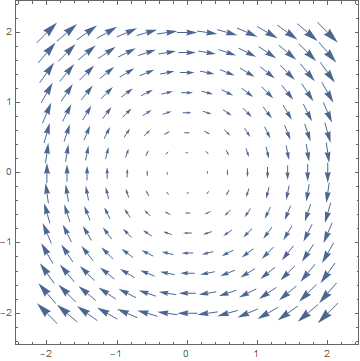
\includegraphics[scale=0.5]{oscillator.png}
	\caption{$x$ è sulle ascisse e $p$ sulle ordinate, le frecce hanno per componenti $\dot{x}$ e $\dot{p}$}
	\label{ellissi}
\end{figure}
Considero un pendolo 1-D con  $m=1$ :
\[H=\f{ p^2}{2}-g \cos(x)		\]
Da cui le linee di flusso sono date dalla curva parametrica $ \gamma=\f{1}{\d t}(\d x,\d p)=(\dot{x},\dot{p})$:
\[\dot{x}=p\]
\[\dot{p}=-g\sin(x)\]
\begin{figure}[h]
	\centering
	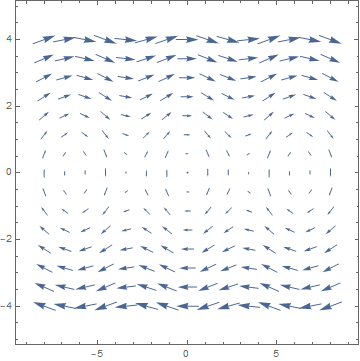
\includegraphics[scale=0.5]{pend1.png}
	\caption{Linee di Flusso per pendolo semplice}
\end{figure}
Si vede che i vari punti di minimo (di $H$) sono $x=2k\pi,\,p=0$, attorno a cui le linee di flusso sembrano quasi quelle di un oscillatore armonico. I punti di minimo sono caratterizzati da $\dot{x}=\dot{p}=0$, visto che tutte le componenti del gradiente di $H$ si annullano in quel punto.
\section{Espansione attorno al minimo}
\label{expand1}
Si vuole studiare il comportamento del sistema attorno ai punti di minimo, espandendo in Taylor e linearizzando.\\Suppongo $\dot{x}=f\arg{x,p}$ e $\dot{p}=g\arg{x,p}$ e che queste funzioni si annullino entrambe in $x_0,p_0$

\[\begin{pmatrix}
\dot{x} \\ 
\dot{p}
\end{pmatrix} \approx\begin{pmatrix}
\partial_x f & \partial_p f \\ 
\partial_x g & \partial_p g
\end{pmatrix} 	\begin{pmatrix}
x-x_0 \\ 
p-p_0
\end{pmatrix}=M\begin{pmatrix}
\delta x \\ 
\delta p
\end{pmatrix} 	\]
Supponendo di diagonalizzare $H$, e detti $\lambda_{1,2}$ i suoi autovalori, si individuano vari casi:
\begin{enumerate}
\item $\lambda_1\le\lambda_2\le 0$ punto di stabilità, i due modi normali decadono esponenzialmente (si hanno delle equazioni del tipo $\delta\dot{z}=\lambda \delta z$)
\item $\lambda_1\ge\lambda_2\ge0$ punto instabile, tutti i vettori appena fuori dal minimo scappano via
\item Nel caso di autovalori complessi si creano spirali:

\begin{figure}[h]
	\centering
	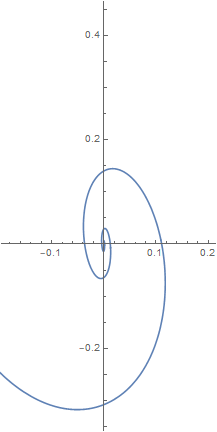
\includegraphics[scale=0.4]{stablespiral.png}
	\caption{esempio di spirale stabile}
\end{figure}
 $\lambda_1=\alpha+i\beta$ e $\lambda_2=\alpha-i\beta$, con $\alpha<0$.\\ Questi due modi normali ruotano in senso opposto attorno al punto e ci cadono esponenzialmente dentro (\textbf{spirale stabile})
 
\item Nel caso precedente, ma con $\alpha=0$ si hanno delle rotazioni attorno al punto detto \textbf{ellittico} senza mai caderci dentro (è il caso del pendolo semplice senza attrito o dell'oscillatore armonico)
\item Analogamente ci possono essere \textbf{spirali instabili} con $\alpha>0$
\end{enumerate}
 Sono dette \textbf{mooncline} sono dette le rette che hanno $\dot{p}=0$ o $\dot{x}=0$.


\begin{exmp}[pendolo con attrito]
Sia $m=1$;
le equazioni per il pendolo con attrito sono:
\[\dot{x}=p\;\;\econg\;\;\dot{p}=-\f{g}{l}\sin\argg{x}-	\gamma p	\]
Quindi le mooncline sono \[p=0\;\;\econg\;\; p=-\f{g}{l\gamma}\sin(x)\] 
Queste traiettorie sono importanti perchè(ad esempio quella con $\dot{p}=0$) separano le due regioni con il segno di $\dot{p}$ positivo o negativo, e quindi la direzione di spostamento di $p$.\\
Analizzando la dinamica di un pendolo, si ha che, ad esempio per alte $p$ iniziali, il decadimento dell'energia (e delle $p$) è esponenziale, e dovuto al termine dominante $\gamma p$, per la posizione invece \[x=\int p \d t\propto\f{1}{\gamma} e^{-\gamma t}\]
Quindi l'andamento a grandi $p$ nello spazio delle fasi sarà una retta di pendenza $\gamma$ (visto che il rapporto fra $p$ e $x$ non dipende dal tempo in questa approssimazione).\\
Dal grafico \ref{frpend} si vede chiaramente cosa succede quando il sistema (in blu) entra dentro una mooncline con $p=0$ (in rosso): il segno di $\dot{p}$ cambia ed infatti la $p$ risale, per poi ricominciare a scendere non appena il sistema esce dalla regione $\dot{p}\ge 0$, intersecando, cioè, un'altra volta la mooncline.
 \\Quando viene dissipata abbastanza energia, si riesce ad avere $p=0$ (la traiettoria interseca l'asse delle $x$ ), ed il sistema interseca l'altra mooncline, con $\dot{x}=0$. \\Attraversando questa regione, la componente $x$ inverte il moto, cioè il pendolo inizia a girare su se' stesso e il moto tende ad una spirale stabile, come si può di nuovo vedere in figura \ref{frpend}\begin{figure}[h]
	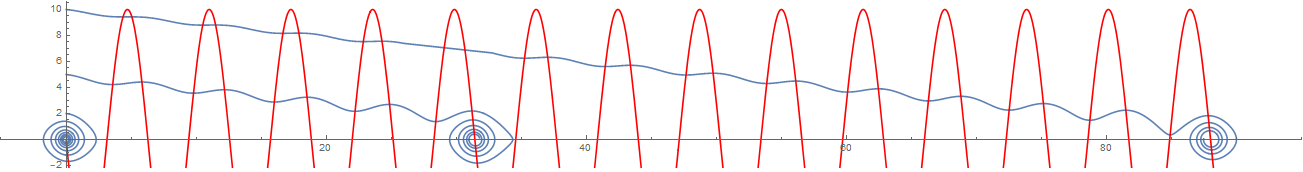
\includegraphics[scale=0.3]{Exm.png}
	\caption{Grafico ottenuto per diversi valori di $p$ iniziali, ovvero $p=10,5,2$, $\gamma=0.1$ e tutti gli altri parametri pari a $1$.In rosso si può vedere disegnata la mooncline (è un seno). Notare che quando il sistema è dentro la mooncline, la $p$ sale, quando è fuori, la $p$ scende; non appena il sistema tocca l'asse delle $x$ resta intrappolato}
	\label{frpend}
\end{figure}
	
\end{exmp}

\begin{exmp}[equazioni di Lotka-Volterra]
Guardo i punti di stabilità delle equazioni di Lotka-Volterra \ref{eq7}: \[\dv{x}{t}=x-x y\:\:\:\:\:\:
\dv{y}{t}=x y-y\]Ce ne sono almeno 2, $(0,0)\econg(1,1)$
Espandendo intorno allo 0, si trova la matrice di stabilità
\[\Op{M}=\begin{pmatrix}
1 &0\\ 
0 & -1
\end{pmatrix} \] 
Quindi si ha un punto di sella: il sistema fugge nella direzione dell'autovettore $\hat{x}$, che ha autovalore $\ge0 $.\\
Espandendo intorno all'altro minimo in  $(1,1)$:
\[\Op{M}=\begin{pmatrix}
0 &1\\ 
-1 & 0
\end{pmatrix} \]
Che ha autovalori $\pm i$ (se la si moltiplica per $i$ si ottiene una matrice di Pauli $\sigma_y$), quindi si ha un punto ellittico (spirale stabile). 
\begin{figure}[h]
	\centering
	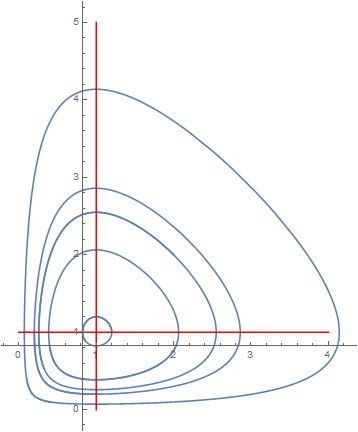
\includegraphics[scale=0.4]{lotka2.png}
	\caption{Equazioni di Lotka-Volterra, con le mooncline in rosso e vari valori del parametro iniziale}
\end{figure}
\end{exmp}


\subsection{Cerchio Limite}
\label{limit}
L'analisi precedente è valida fino al prim'ordine, il che pone limiti ben precisi. \\Specialmente il caso di punto ellittico, dove le traiettorie dovrebbero essere stabili, è molto soggetto, su lunghi tempi, all'influenza degli altri ordini perturbativi (mentre invece, stando sufficientemente vicini al punto, i punti stabili e instabili restano tali anche in presenza di altri ordini perturbativi, essendo definiti da una disuguaglianza, quindi con un certo "margine di errore").
\\Ad esempio, il sistema :
\begin{align}
\dot{x}=x+y-x(x^2+y^2)
\\\dot{y}=-x+y-y(x^2+y^2)
\end{align}
ha un comportamento che non si può estrarre da un'analisi perturbativa: la matrice di stabilità per questo sistema intorno all'origine è
\[\Op{M}=\begin{pmatrix}
1 &-1\\ 
1 & 1
\end{pmatrix} \]
cioè ha autovalori $1\pm i$, quindi l'origine è un punto instabile. \\Passando a variabili polari si riesce a risolvere il sistema in modo esatto:
\[\rho^2=x^2+y^2\implies\dot{\rho} \rho=x^2+yx-x^2(x^2+y^2)-xy+y^2-y^2(x^2+y^2)=			\]
\[=x^2+y^2-x^4-y^2-2x^2y^2=\rho^2-\rho^4	\implies \dv{\rho^2}{t}=2\rho^2-2\rho^4		\]

Questa equazione si può integrare:
\[\int\f{\d \rho^2}{\rho^2(1-\rho^2)}=\int\d \rho^2\left(\f{1}{\rho^2}+\f{1}{1-\rho^2}\right)=2(t-t_0)			\]
\[\ln(\f{\rho^2}{1-\rho^2})=2(t-t_0)\]
\[\rho^2=\f{e^{2(t-t_0)}}{1+e^{2(t-t_0)}}		\]
Il che vuol dire che il sistema si avvicina esponenzialmente al cerchio di raggio $1$ centrato nell'origine: si ha un \textbf{cerchio limite}. Il fatto che la regione di equilibrio non sia stavolta un punto, ma un intero cerchio, non è chiaramente ottenibile da un'espansione in Taylor
\section{Trasformazioni Canoniche}

Supponiamo di avere un sistema Hamiltoniano n-dimensionale, che obbedisce cioè alle equazioni di Hamilton:
\[\dot{\vec{x}}=\pdv{H}{\mom}			\]

\[\dot{\mom}=-\pdv{H}{\pos}			\]
Che possono essere riscritte utilizzando un'unico vettore 2n-dimensionale:
\[\begin{cases}
	z_i=x_i \:\:\:i\le n\\
z_i=p_i \:\:\:i> n
\end{cases}\]
Introducendo la seguente matrice  $n\cross n$ \[\zeta=\begin{pmatrix}
0&\unit\\
-\unit&0
\end{pmatrix}\]
Le equazioni si riducono a \[\dot{z}_i=\zeta_{ij}\pdv{H}{z_j}\]
Vale inoltre $\zeta^2=\unit$, quindi, moltiplicando ambo i membri per $\zeta$
\[\zeta_{li}\dot{z}_i=\pdv{H}{z_j}\]
\begin{defn}[flusso Hamiltoniano]\label{flux}
	Dato un vettore $z_i$ nello spazio delle fasi, questo si muove nella direzione $J_i=\dot{z}_i$, dove $\vec{J}$ è definito come flusso Hamiltoniano. 
	\[\vec{J}=\zeta\vec{\nabla}_z	H(\vec{z})	\]
	In generale, il flusso si può definire per una qualunque funzione scalare delle coordinate: 
	\[J_A=\zeta\vec{\nabla}_z	A(\vec{z})\]
\end{defn}
\begin{defn}[parentesi di Poisson]
	Date due funzioni delle coordinate, $f\econg g$, si definiscono le parentesi di Poisson:
	\[\{f,g\}=\pdv{f}{q_i}\pdv{g}{p_i}-\pdv{g}{q_i}\pdv{f}{p_i}=\pdv{f}{z_i}\pdv{g}{z_j}	\zeta_{ij}\]
	Le parentesi di Poisson sono antisimmetriche (lo si vede scambiando gli indici $i,j$ e notando che $\zeta$ è antisimmetrica), inoltre l'evoluto temporale di una quantità è:
	\[	\dv{f}{t}=\pdv{f}{z_i}\dot{z}_i=\pdv{f}{z_i}\pdv{H}{z_j}\zeta_{ij}=\{f,H\}	\]
\end{defn}
	
\begin{defn}[trasformazioni canoniche]
Sono quei cambi di coordinate $z_i\rightarrow Z_i(\vec{z})$ che preservano le equazioni di Hamilton, quindi tali che valga ancora:
\[\dot{Z}_i=\zeta_{ij}\pdv{H}{Z_j}\]
\end{defn}
Sia $J^{-1}_{lm}=\pdv{z_l}{Z_m}$ lo Jacobiano della trasformazione di coordinate, se vogliamo che la trasformazione sia canonica deve valere:
\[\dot{Z}_i=\zeta_{ij}\pdv{H}{Z_j}=\zeta_{ij}\pdv{H}{z_l}\pdv{z_l}{Z_j}=\zeta_{ij}J^{-1}_{lj}\zeta_{lm} \dot{z}_m		\]
Ma vale anche:
\[\dot{Z}_i=\pdv{Z_i}{z_j}\dot{z}_j=J_{ij}\dot{z_j}	\]
Da cui si ha l'identità fra matrici:
\[\zeta \left(J^{-1}\right)^t \zeta=J		\]
Detta altrimenti la condizione di canonicità è
\boxedeq{canonical}{J\zeta J^t=\zeta}
Le matrici $J$ che rispettano questa proprietà sono dette matrici \textbf{simplettiche}, e formano un gruppo.
Facendo il determinante di ambo i membri e notando che  $\text{Det}(\zeta
)=1$:
\[\text{Det}(J)^2=1\]

In realtà si può dimostrare che vale per matrici simplettiche la condizione più forte 
\[\text{Det}(J)=1\]

\begin{thm} [autovalori matrici simplettiche]
	\label{Sim}
	Gli autovalori di una matrice simplettica soddisfano la relazione:
	\[\lambda_i=\lambda_j^{-1}\]5
	ovvero dato un qualunque autovalore, anche l'inverso di quell'autovalore è un autovalore
\end{thm}

\begin{proof}
	Notiamo anzitutto che vale $\zeta=\zeta^{-1}$, quindi la condizione di matrice simplettica diventa:
	\[\zeta^{-1} J\zeta=\left(J^{-1}\right)^t		\]
	Il membro sinistro è una trasformazione di similitudine su $J$, significa che lascia il suo spettro invariato; quindi gli autovalori di $J$ sono gli stessi di $\zeta J\zeta=\left(J^{-1}\right)^t$.\\Anche fare la trasposta di una matrice non cambia lo spettro, quindi gli autovalori di $J$ sono gli stessi di $J^{-1}$ e quindi per ogni autovalore $\lambda$ ci deve essere anche l'autovalore $\lambda^{-1}$
	
	
	
	
	
	
\end{proof}
\begin{obs}
questo teorema implica che per ogni autovalore ce n'è un'altro distinto che è il suo reciproco, tranne che nei casi $\lambda=\pm 1$. Si possono eliminare i casi $\lambda=-1$ con trasformazioni di parità, ed infine notare che le trasformazioni di parità  permesse
 cambiano contemporaneamente il segno di $x_i$
e di $p_i$, quindi hanno autovalori $-1$ a coppie. (questa non è una dim formale ma dà un'idea del perchè $\det(J)=1$)

\end{obs}
Una implicazione del fatto che le matrici simplettiche hanno determinante unitario è che \textbf{preservano il volume dello spazio delle fasi}.\\
Ovvero, usando la notazione $\vec{p}\econg\vec{q}$ per indicare coordinate e impulsi coniugati si ha:
\[\int  \d^n\mom	\;	\d^n\vec{q}=\int  \d^n\vec{P}\;\d^n\vec{Q}\det(J)=\int  \d^n\vec{P}\;\d^n\vec{Q}	\]
Si può dimostrare che le trasformazioni canoniche sono indotte da funzioni generatrici (che possono essere di 4 tipi diversi, a seconda di cosa prendono per argomento), la più usata è la $F_2$. Indicando con indici piccoli le vecchie variabili e con quelli grandi le nuove variabili:
\[F_2(\vec{q},\vec{P},t)\:\:\:\:\:\:\vec{p}=\pdv{F_2}{\vec{q}}\:\:\:\vec{Q}=\pdv{F_2}{\vec{P}}\quad     H'(\vec{Q},\vec{P})=H(\vec{q}(\vec{Q},\vec{P}),\vec{p}(\vec{Q},\vec{P})+\pdv{F_2}{t}\]
L'identità come cambio di variabili si ottiene ad esempio scegliendo $F_2=\vec{q}\vec{P}$
\begin{exmp}[evoluzione temporale]
	L'evoluzione temporale è una trasformazione canonica; discende dal fatto che le equazioni canoniche sono rispettate a tutti i tempi, quindi se valgono per $\vec{z}(t)$, allora varranno per $z(T+t)$ cioè per le coordinate generalizzate traslate (o evolute) di un tempo $T$.\\
	Più esplicitamente, basta notare che l'evoluzione temporale per $\d t$ è generata da $F_2= \vec{q}\vec{P}+H(\vec{q},\vec{P})\d t$.
	\end{exmp}

\begin{exmp}\label{exmp2}
	
	
	Dimostriamo che l'evoluzione temporale lascia invariato l'integrale della forma \[\oint p_i \d q_i-H\d t\]uso la notazione per coordinate e momenti unficate $\begin{pmatrix}
	\vec{q}\\\vec{p}
	\end{pmatrix}=\vec{z}$. Il mio spazio di integrazione è lo spazio delle fasi "esteso" con anche il tempo $t$ come variabile.
	\[\oint p_i \d q_i-H\d t=\oint\left(\f{1}{2}p_i \d q_i-\f{1}{2}q_i \d p_i\right)-\oint H\d t=\oint	\f{1}{2}\zeta_{ij} z_i \d z_j-H\d t	\]
Calcolo la variazione $\delta$ sotto traslazione temporale per un tempo $\delta t$
	\[\delta\oint\f{1}{2}	\zeta_{ij} z_i \d z_j-H\d t=\delta t\oint\f{1}{2}	\zeta_{ij} \dot{z}_i \d z_j+\f{1}{2}\zeta_{ij} {z}_i \d \delta z_j-\delta t\pdv{H}{t}\d t\]
	Integro per parti il secondo addendo: (tutti i differenziali totali integrati fanno zero perchè il cammino è chiuso)
	\[	\oint\zeta_{ij} {z}_i \d \delta z_j =\oint	\zeta_{ij} \d \left( {z}_i\delta z_j	\right)	-\oint \zeta_{ij} \delta z_j \d z_i=-\oint \zeta_{ij} \delta z_j \d z_i=\oint \zeta_{ij} \delta z_i \d z_j=\]
	Nell'ultimo passaggio si è sfruttata l'antisimmetria di $\zeta$.
	\[=\delta t \oint \zeta_{ij} \dot{z_i} \d z_j	=\delta t \oint \zeta_{ij} \pdv{H}{z_l} \zeta_{il} \d z_j\]
	Ora ritorniamo all'equazione iniziale, ricordo che $\zeta^2_{il}=\zeta_{ij}\zeta_{jl}=\delta_{il}$:
	\[\delta\oint\f{1}{2}	\zeta_{ij} z_i \d z_j-H\d t=\oint\delta t	\zeta_{ij} \dot{z}_i \d z_j-\delta t\pdv{H}{t}\d t=\]\[=\oint\delta t	\zeta_{ij} \dot{z}_i \d z_j-\delta t\pdv{H}{t}\d t=\delta t\oint	\zeta_{ij} \pdv{H}{z_l} \zeta_{il} \d z_j-\delta t\pdv{H}{t}\d t=-\delta t\oint	 \pdv{H}{z_l} \delta_{jl} \d z_j-\delta t\pdv{H}{t}\d t=\]\[=-\delta t\oint\left( \pdv{H}{z_j}  \d z_j+\pdv{H}{t}\d t\right)=	\delta t\oint\left( \d H\right)=0\]
	Quindi si ha che la forma\[ p_i \d q_i-H\d t\]
	rimane costante nel tempo.
\end{exmp}
\section{Equazione di Hamilton-Jacobi}
Un cambio di variabili che permette di risolvere l'equazione del moto è ad esempio un cambio di variabile che elimini la dipendenza dell'Hamiltoniana da una variabile, il che corrisponde a dire che il suo impulso coniugato si conserva.\\
Chiamiando $S=F_2$ la funzione generatrice che descrive questo cambio di coordinate e detti $\vec{\alpha}$ i nuovi momenti coniugati: la nuova Hamiltoniana deve dipendere solo da questi
\boxedeq{tindHJ}{H\left(\vec{q},\f{\partial S(\vec{q},\vec{\alpha})}{\partial\vec{q}}\right)=H'(\vec{\alpha})}
Che prende il nome di \textbf{Equazione time-independent di Hamilton-Jacobi}.\footnote{
Il fatto che $H(q,J)$ non dipende da $q$ vuol dire che anche $H(q,(\phi,J),J)$ non dipende da $\phi$}



La solita equazione di Hamilton Jacobi si ottiene imponendo un cambio di variabili dipendente dal tempo che  annulli in ogni istante l'Hamiltoniana nelle nuove variabili (questo non si può fare in generale con un cambio di variabili time independent perchè si ha $H\argg{\vec{q},\mom}=H\left(\vec{\beta}\arg{\vec{q},\mom},\vec{\alpha}\arg{\vec{q},\mom}\right)\ne0$)
\\ Imponendo che la nuova hamiltoniana sia nulla:
\[0=H'=\pdv{S}{t}+H\left(\vec{q},\f{\partial S}{\partial\vec{q}}\right)\]
Che è l'equazione di Hamilton-Jacobi solita.
\\Ritornando all'equazione time-independent, supponiamo di voler scrivere \[S(\vec{q}\arg{t},\vec{\alpha}\arg{t})\implies\d S=\pdv{S}{\vec{q}}\d\vec{q}\]
Dove si è usato il fatto che gli $\alpha_i$ non variano nel tempo.
\[\d S=\sum_i \pdv{S}{q_i}\d q_i=\sum_i p_i\argg{\vec{q},\vec{\alpha}}\d q_i\implies S=\sum_i\int_{t_0}^t	p_i\argg{\vec{q},\vec{\alpha}}\d q_i	\]
e l'integrale è fatto sulla traiettoria classica.

\boxedeq{tindHJ2}{S=\sum_i \int_{t_0}^t	p_i\d q_i}
\subsection{Soluzione di HJ in 1-D}
Supponiamo di avere un solo grado di liberà, quindi solo una coordinata e un impulso coniugato.
\\ C'è un grado di liberà nella scelta di $H(\alpha)$ perchè, prendendo come nuovo impulso $\alpha\rightarrow \alpha'(\alpha)$ (che è una trasformazione canonica se cambio consistentemente le coordinate), ho che anche il nuovo impulso è conservato perchè funzione di una quantità costante nel tempo. Quindi posso scegliere $H(\alpha)$ come generica funzione (l'importante è che sia non-nulla).\\ La scelta più semplice è\[H(\alpha)=\alpha\]
A questo punto risolvo l'equazione \ref{tindHJ}; usando l'equazione Hamilton per la nuova coordinata:
\[\dot{\beta}=\pdv{H}{\alpha}=1\implies\beta\arg{t}=t-t_0			\]
Uso l'equazione \ref{tindHJ2}:
\[t-t_0=\beta=\pdv{S}{\alpha}=\pdv{\alpha} \int_{t_0}^t	p\d q\]
Immaginando l'Hamiltoniana della solita forma
\[H=\f{p^2}{2m}+V\arg{q}=\alpha\implies p=\sqrt{2m\left(\alpha-V\arg{q}\right)}			\]
Rimettendo tutto insieme:
\[t-t_0=\pdv{\alpha} \int_{t_0}^t\sqrt{2m\left(\alpha-V\arg{q}\right)}	\d q=
\int_{t_0}^t\sqrt{\f{m}{2\left(\alpha-V\arg{q}\right)}}	\d q(t)
\]
$\alpha$ è fissata dalle condizioni iniziali (è l'energia): integrando in $q$ ed invertendo si trova $q(t)$.
\subsection{Variabili Azione-Angolo}
In una dimensione, se il moto è limitato, allora è periodico, perchè esiste almeno un integrale del moto, $H$, che forza il moto su di una traiettoria. Vorremmo un cambio di variabili tale che la nuova coordinata $\theta$ esprima una quantità analoga all'angolo percorso sulla traiettoria chiusa, tale che dopo ogni giro aumenti di $2\pi$  e che aumenti linearmente nel tempo ($\pdv{H}{I}=const$ quindi l'impulso coniugato $I$ si deve conservare: $H=H(I)$).\[2\pi=	\oint\d \theta	\]
Usando la funzione generatrice:
\[\theta= \pdv{S(q,I)}{I}	\]
\[2\pi=	\oint \d \theta(q,I)=\oint \pdv{\theta}{q} \d q+ \pdv{\theta}{I} \d I	=\]
Dato che l'impulso coniugato a $\theta$ è conservato sulla traiettoria, $\d I=0$
\[=\oint \pdv{\theta}{q} \d q=\oint \pdv[2]{S(q,I)}{q}{I} \d q=\pdv{I}\oint \pdv{\theta(q,I)}{q} \d q=\pdv{I}\oint p(q,I) \d q\]

Da cui si ottiene:
\[ 2\pi=		\pdv{I}\oint p \d q\implies\]
\boxedeq{Actionangle}{2\pi I=\oint p \d q	}
\begin{obs}

La variabile angolo sembra molto analoga alla coordinata tempo fatta imponendo $H(\alpha)=\alpha$, perchè aumentano entrambe linearmente, il rapporto è, dato un periodo $T$:
\[\f{\Delta \alpha}{\Delta \theta}=\f{T}{2\pi}=\f{1}{\omega(I)}			\]
Il punto è che la frequenza $\omega(I)$ dipende dall'energia, quindi il rapporto fra le due variabili non è costante (se lo fosse sarebbero praticamente la stessa variabile)
\end{obs}

Il procedimento per passare alla variabile angolo è fare l'integrale \ref{Actionangle} sfruttando l'integrale del moto $H(p,q)=E$:\[\oint 	p(E,q) \d q		\] 
\begin{exmp}[oscillatore armonico]\label{exmp1}
	Nel caso dell'oscillatore armonico, con periodo costante $\omega$, si trova che $\theta$ non dipende dalle vecchie variabili, mentre vale 
	\[I=\f{1}{2\pi} \sqrt{{2m}{E}}\oint {\sqrt{1-\f{m}{2 E} \omega^2 q^2}}	\d 	q	\]
	Cambio variabile\footnote{l'integrale lo faccio con un cambio di variabili $x=\sin(t)$, inoltre su un mezzo periodo posso scambiare $\sin^2\ra\f{1}{2}$}:
	\[q=\sqrt{\f{2 E}{m}}\f{1}{\omega} x\implies I=\f{
	E}{\pi\omega} \oint {\sqrt{1-x^2}}	{\d x}=\f{
	E}{\omega\pi}\,2\,\int_{-1}^1 {\sqrt{1-x^2}}	{\d x}=\f{E}{\omega}	\]
In sostanza si ha :
\[\theta=\omega t+\delta\]
\[I=\f{E}{\omega}\]
Volendo eprimere le vecchie variabili in funzione delle nuove:
\[q=\f{1}{\omega}\sqrt{\f{2E}{m}} \cos(\theta-\delta) 	=\sqrt{\f{2I}{m\omega}} \cos(\theta-\delta) 		\]
\[p=\sqrt{{2E}{m}} \sin(\theta-\delta)=\sqrt{{2I\omega}{m}} \sin(\theta-\delta) 	\]
\end{exmp}
\begin{defn}[Hamiltoniana Separabile]
	Un'Hamiltoniana del tipo $H(q_1,q_2,p_1,p_2,\ldots)$ è detta separabile se vale:
	\[H(q_1,q_2,p_1,p_2,\ldots=H_1(q_1,p_1)+H_2(q_2,p_2)+\ldots\]
	Ovviamente la nozione di separabilità dipende anche dalla scelta delle variabili
	
\end{defn}
Nel caso in cui un'Hamiltoniana sia separabile in sistemi 1-D, si può fare il cambio di variabile angolo-azione per tutti i sottosistemi. \\
In generale, un sistema $n$ dimensionale è detto \textbf{totalmente integrabile}  se esistono $n$ integrali del moto $G^l$ indipendenti(non posso scrivere un integrale del moto come funzione di altri integrali del moto) che sono involuti l'un l'altro, ovvero tali che le loro parentesi di Poisson si annullino:
\[\{G^l,G^m\}=0\]
Se il sistema ha $n$ vincoli, si muoverà su una varietà $n$ dimensionale (dei $2n $ gradi di libertà iniziali gliene restano solo $n$).\\
In particolare, la varietà sarà punto per punto perpendicolare ai gradienti dei vari integrali del moto (fatti nelle coordinate generalizzate); infatti, dato che il vettore $\dot{z}_i$ è per ipotesi tangente alla varietà dove si svolge il moto
\[\dot{z}_i\pdv{G^l}{z_i}=\dv{ G^l}{t}=0\]
Siano $\xi^l_i=\zeta_{ij}\pdv{G^l}{z_j}$ $n$ vettori indipendenti ricavati dagli integrali del moto (sono indipendenti perchè i gradienti dei vari integrali del moto devono essere indipendenti fra loro per ipotesi).
\\Allora si ha che tutti i vettori $\vec{\xi}^l$ giacciono lungo la varietà $n$-dimensionale. Per dimostrarlo, basta far vedere che sono ortogonali ai gradienti di tutti gli invarianti del moto $G^m$.
\[\xi^l_i\pdv{G^m}{z_i}=\partial_i G^m \partial_jG^l \zeta_{ij}=\{G^m,G^l\}=0		\]
Quindi si ha, punto per punto della varietà su cui si svolge il moto, definito un campo vettoriale con $n$ vettori indipendenti. La varietà deve quindi essere, per il teorema della palla pelosa\footnote{Detto anche teorema di Poincarè Hopf, dice che se posso costruire $n$ campi vettoriali linearmente indipendenti tangenti ad una varietà $n$ dimensionale, allora questa ha la topologia di un toro}, un toro.
\\Supponiamo quindi di aver trovato gli $n$ integrali del moto e di averli usati per passare alle varibili azione-angolo $\theta_i,I_i$: si può fare una specie di serie di Fourier delle coordinate iniziali, questo si può fare perchè le vecchie coordinate $q_{i\,\vec{\theta,\vec{I}}}$ sono periodiche nei $\theta_i$ con periodo $2\pi$ (per definizione di variabili angolo):
\[a_{j}(\,\vec{k})=\f{1}{(2\pi)^n}\int_0^{2\pi} \d \theta_1\int_0^{2\pi} \d \theta_2\int_0^{2\pi} \d \theta_3\ldots q_j e^{-i \vec{\theta}\vec{k}}			\]
Dove $\vec{k}$ è un vettore di numeri \textbf{INTERI}.\\
Questi sono i coefficienti della serie di Fourier. Vale quindi:
\[q_j=\sum_{\vec{k}\in \mathbb{Z}^n} a_j(\vec{k})	e^{i \vec{k}\vec{\theta}}			\]
Ma usando questa decomposizione, si può sostituire l'evoluzione nel tempo dei vari $\theta$:\[\theta_i(t)=\omega_it+\delta_i\]
Quindi si ottiene

\boxedeq{Eq8}{q_j(t)=\sum_{\vec{k}\in \mathbb{Z}^n} a_j\left(\vec{k}\right)	e^{i (k_l \omega_lt+k_l\delta_l)}	}
Da questa forma è chiaro che, affinchè il moto sia periodico, deve esistere un $t$ tale che \[\omega_i t=2\pi n	\:\:\:\forall i	\]
Detto in altri termini, i rapporti di tutte le frequenze devono essere razionali, altrimenti il moto sul toro non è periodico
\subsection{Teoria Perturbativa}
Supponiamo di avere un'Hamiltoniana integrabile $H_0$ a cui si aggiunge un'altra piccola Hamiltoniana $\epsilon H_1$ perturbativamente ($\epsilon\ll1$). Supponendo di essere passati alle variabili azione angolo , si ha:
\[H=H_0(I)+\epsilon H_1(\theta,I)		\]
Vogliamo un cambio di variabili $(\theta,I)\rightarrow(\phi,J)$ che, al prim'ordine, risolva la nuova Hamiltoniana, ovvero $H=H(J)+o(\epsilon)$.
\\ Sia $S$ la funzione generatrice; all'ordine $0$ deve essere l'identità:
\[S(\theta,J)=\theta J+\epsilon S_1\]
Ora impongo l'equazione \ref{tindHJ} (chiamo $K(J)$ la nuova Hamiltoniana in funzione di solo $J$ per evitare casini, però essendo il cambio di variabili time independent, è proprio la vecchia Hamiltoniana totale $H_0+\epsilon H_1$ con le nuove variabili):
\[K(J)=	H_0\left(\pdv{S\arg{\theta, J}}{\theta}\right)+\epsilon H_1\left(\theta,\pdv{S\arg{\theta, J}}{\theta}\right)		\]
Usando l'espansione in serie di $S=S_0+\epsilon S_1$:
\[K(J)=H_0(J+\epsilon \pdv{S_1}{\theta})+\epsilon H_1(\theta,\pdv{S_0}{\theta})\]
Supponiamo di poter espandere $H_0$ in serie di $\epsilon$:
\[K(J)=H_0(J)+\epsilon \pdv{S_1}{\theta} \left.\pdv{H_0}{I}\right|_{I=J}+\epsilon		 H_1(\theta,\pdv{S}{\theta})\]
Adesso faccio due cose: espando $K(J)=K_0+\epsilon K_1$ in potenze di $\epsilon$ e ricordo che, all'ordine 0 $\dot{\theta}=\omega_0(I)=\pdv{H_0}{I}$: inserendo queste due cose, e notando che gli ordini 0 si cancellano ($\left.H_0(I)\right|_{I=J}=K_0(J)$), rimane, all'ordine $\epsilon$
\[K_1=\omega_0(J)	\pdv{S_1}{\theta} +H_1(\theta,J)		\]
Ho anche sostituito in $H_1$ $I=J$, visto che quel pezzo era già al prim'ordine.
\\Adesso è l'ora del truccaccio, fin'ora si trattava solo di applicare l'equazione \ref{tindHJ}; infatti abbiamo due funzioni sconosciute $K_1$ ed $S_1$, quindi il problema non è ancora risolvibile. Il truccaccio sta nel fatto che $H_1$ è periodico in $\theta$. Questo perchè si ha $H_1(q,p)$ ma $q\econg p$ sono periodiche in $\theta$, quindi anche $H_1$ lo sarà. Ma se $H_1$ è periodica, visto che è l'unico dato del problema che abbiamo, tutto il problema deve essere periodico in $\theta$, quindi anche $S_1$ e $K_1$:
 integro ambi i membri da $0$ a $2\pi$
 
 \[\int_0^{2\pi} K_1(J)\d	\theta=2\pi K_1(J)=\int_0^{2\pi} \pdv{\theta} \left[\omega_0(J)	S_1(\theta,J)\right]\d	\theta+\int_0^{2\pi}H_1(\theta,J)\d	\theta=\]\[=\omega_0(J)	S_1(2\pi,J)-\omega_0(J)	S_1(0,J)+\int_0^{2\pi}H_1(\theta,J)\d	\theta=\int_0^{2\pi}H_1(\theta,J)\d	\theta	\]
Usando la periodicità di $S_1$.
Da cui \boxedeq{bohutile}{K_1(J)=\bar{H_1}=\f{1}{2\pi}	\int_0^{2\pi}H_1(\theta,J)\d	\theta\quad \quad\quad \omega'(J)=\omega_0(J)+\f{\epsilon}{2\pi}\int_0^{2\pi} \pdv{H_1(\theta,I=J)}{J}\d \theta	}
Questo permette di chiudere il problema per quadratura, ora risolvo per trovare $S_1$
\[S_1=\int\f{1}{\omega_0(J)}(\bar{H_1}(J)-H_1(\theta,J)\d \theta+ \psi(J)			\]
Dove $\psi$ è una generica funzione di $J$.
\\ Visto che le cose sono periodiche, conviene espandere tutto in serie di Fourier:
\[H_1=\sum_{k=-\infty}^{\infty}	A_k(J) e^{ik\theta}		\]
Da cui si ha anzitutto che \[\bar{H}=A_0\]
Si può scrivere, tenendo conto di questo fatto e dell'integrale in $\theta$
\[S_1(\theta,J)=\f{1}{\omega_0(J)}\sum_{k\in\mathbb{Z}\setminus 0}	\f{iA_0}{k}	e^{ik\theta}+\psi(J)	\]

Ora si può ricavare la nuova variabile angolo $\phi$
\[\phi=\theta+\pdv{{S_1}\arg{\theta,J}}{J}\]
La componente a $k=0$ di $S_1$ , ovvero $\psi(J)$, non fa altro che dare uno sfasamento nel cambio di variabile variabile $\theta\ra\phi$:
\[\delta_\phi=\pdv{\psi}{J}		\]
Quindi la si  può riassorbire nella definizione di $\phi$ e porre $=0$.
\begin{exmp}[oscillatore anarmonico]
	Supponiamo di avere \[H=\f{p^2}{2m}+\f{1}{2}q^2 m\omega^2+\epsilon \lambda q^4		\]
	In variabili azione angolo, prende la forma (uso \ref{exmp1}):
	\[H=\omega I+ \epsilon\lambda	\left(\f{2I}{m\omega}\right)^2 \sin^4(\theta)	\]
	Usando il risultato precedente:
	\[K_1=\f{1}{2\pi}\int_0^{2\pi} 	\lambda	\left(\f{2J}{m\omega}\right)^2 \sin^4(\theta)\d \theta		\]
	\[\int_0^{2\pi }	\sin^4(\theta)\d \theta=\int_0^{2\pi }	\sin^2(\theta)(1-\cos^2(\theta))\d \theta=\int_0^{2\pi }	\sin^2(\theta)-\f{1}{4} \sin^2(2\theta)\d \theta=	\]
	Usando il fatto che il valor medio del seno quadro è $\f{1}{2}$:
	\[=\pi-\f{\pi}{4}=\f{3}{4}\pi		\]
	Da cui \[K_1=\f{3}{8}	\lambda	\left(\f{2J}{m\omega}\right)^2 \]
	Ricordando che $K$ è l'Hamiltoniana nelle nuove variabili:
	\[\dot{\phi}(J)=\omega(J)=\pdv{K}{J}=\theta+\epsilon\pdv{K_1}{J}=\omega+3\epsilon\lambda \f{J}{\omega^2}\]
	Per esprimere la nuova frequenza in funzione dell'energia bisogna invertire la relazione $K_1(J)=E(J)$ (basta farlo al prim'ordine):
	\[E(J)=\omega J+\f{3}{2}\lambda\left(\f{J}{m\omega}\right)^2\approx\omega J+\f{3}{2}\lambda\left(\f{E \omega}{m\omega}\right)^2	\implies J(E)= \f{E}{\omega}- \f{3\lambda}{2\omega}\left(\f{E}{m}\right)^2	\]
	E reinserire tutto nella frequenza per avere $\omega(E)$.




\end{exmp}
In 1-D è tutto integrabile, quindi questi risultati non sono una novità, è interessante generalizzare il tutto in n dimensioni.
\[H=H_0(\vec{I})+\epsilon H_1 (\vec{\theta}+\vec{I}) 		\]
Il termine perturbativo deve essere periodico in ogni componente del vettore $\theta$, quindi si può decomporre in serie di Fourier:
\[H=H_0+\sum_{k\in\mathbb{Z}^n}	A_{\vec{k}}	(\vec{J})	e^{i \vec{k}\vec{\theta}		}	\]
Procedendo come prima (siano $\omega_{0i}$ le frequenze all'ordine $0$ per le varie componenti di $\theta$):
\[K_1(\vec{J})=\omega_{0i}(\vec{J})\pdv{S_1}{\theta_i}+	\sum_{k\in\mathbb{Z}^n}	A_{\vec{k}}	(\vec{J})	e^{i \vec{k}\vec{\theta}	}		\]
\[K_1(\vec{J})=A_{\vec{0}}\]
Scompongo $S_1$ in fourier:

\[S_1=	\sum_{k\in\mathbb{Z}^n}	g_{\vec{k}}	(\vec{J})	e^{i \vec{k}\vec{\theta}	}\implies \pdv{S_1}{\theta_i}\omega_{0i}=\sum_{k\in\mathbb{Z}^n}	{g_{\vec{k}}	(\vec{J})}{i {k_i}\omega_{0i}}	e^{i \vec{k}\vec{\theta}	}\]\[\pdv{S_1}{\vec{\theta}}\vec{\omega_0}=\sum_{k\in\mathbb{Z}^n}{i\vec{k}\vec{\omega_o}}	g_{\vec{k}}	(\vec{J})	e^{i \vec{k}\vec{\theta}	}\]
Inserendo tutto nell'equazione con $K_1$, si vede che :
\[\sum_{k\in\mathbb{Z}^n}{i\vec{k}\vec{\omega_o}}	g_{\vec{k}}	(\vec{J})	e^{i \vec{k}\vec{\theta}	}+	\sum_{k\in\mathbb{Z}^n\setminus\vec{0}}	A_{\vec{k}}	(\vec{J})	e^{i \vec{k}\vec{\theta}	}=0	\implies g_{\vec{k}}=-\f{A_{\vec{k}}}{i\vec{k}\vec{\omega}_0}	\]
Da cui
\[I_i=J_i+\epsilon\pdv{S_1}{\theta_i}=J_i-\epsilon		\sum_{k\in\mathbb{Z}^n\setminus \vec{0}}k_i\f{{A_{\vec{k}}}}{\vec{k}\vec{\omega}_0}(\vec{J})	e^{i \vec{k}\vec{\theta}	}	\]
Scrivendo tutto in forma vettoriale (l'equazione di prima era scritta a una componente $i$):
\boxedeq{PertN-D}{\vec{I}=\vec{J}-\epsilon		\sum_{k\in\mathbb{Z}^n\setminus \vec{0}}\vec{k}\f{{A_{\vec{k}}}\arg{\vec{J}}}{\vec{k}\cdot\vec{\omega}_0}	e^{i \vec{k}\vec{\theta}	}}
E inoltre \[S_1=-	\sum_{k\in\mathbb{Z}^n\setminus\vec{0}}	\f{A_{\vec{k}}(\vec{J})}{i\vec{k}\cdot\vec{\omega}_0}	e^{i \vec{k}\vec{\theta}	}\]
Ora è importante notare che il denominatore ${i\vec{k}\vec{\omega}_0}$ si annulla se le frequenze sono in rapporto commensurabile fra loro (basta che almeno 2 lo siano), il che annulla tutto l'approccio perturbativo, visto che c'è una divergenza.
Tuttavia, anche nel caso di frequenze irrazionali (termine che si adotta per dire incommensurabili fra loro), può capitare che esista un $\vec{k}$ per cui
\[\vec{k}\cdot\vec{\omega}\approx0\]
ovvero che le frequenze siano sì incommensurabili, ma di poco, ed esistono numeri razionali che approssimano "bene" il loro rapporto. In questi casi, il denominatore nella formula \ref{PertN-D}, pur non annullandosi, può diventare molto piccolo per certi $\vec{k}$, e se per quel $\vec{k}$ si ha $A_{\vec{k}}$ non abbastanza piccolo per compensare, ci può essere un'esplosione del termine corrisponente, vanificando tutto l'approccio perturbativo.\\ Come stabilire quanto bene un rapporto può essere approssimato da un numero razionale? Il trucco sta nell'espansione in frazioni continue.\\
In generale per ogni $\sigma\in\mathbb{R}$ esiste un'espansione del tipo:
 \[\sigma=a_0+\cfrac{1}{a_1+\cfrac{1}{a_2+\cfrac{1}{a_3+\ldots}}}\]
 dove la sequenza termina solo per numeri razionali e con $a_n\in\mathbb{N}\setminus 0$.\\
In particolare la serie per un numero razionale sarà del tipo $[a_0,a_1,\ldots,\infty]$, questo perchè l'infinito rende trascurabili tutti i termini successivi nelle frazioni.
\\Per numeri irrazionali ben approssimati da frazioni, si ha che ad un certo punto nell'espansione comparirà un numero molto grosso, che renderà trascurabili tutti i termini successivi; viceversa un numero con termini nella sua espansione tutti molto piccoli sarà "molto" irrazionale.\\ Alla peggio, si possono avere tutti i termini uguali ad $1$ ($0$ non va bene, fa esplodere tutto):
\[\phi=\cfrac{1}{1+\cfrac{1}{1+\cfrac{1}{1+\cfrac{1}{1+\cfrac{1}{1+\cfrac{1}{1+\ldots}}}}}}\]
in particolare si ha la relazione di ricorrenza
\[\phi=\frac{1}{1+\phi}\implies\phi+\phi^2=1\implies\phi=\f{1+\sqrt{5}}{2}\] 
questa costante è detta sezione aurea.\\
Il problema di avere termini esplosivi nell'espansione  \ref{PertN-D} prende il nome di \textbf{problema dei piccoli divisori} ed è seriamente grave perchè i numeri $\vec{\omega}_0(\vec{J})$, sono arbitrariamente vicini a numeri razionali, al variare del punto $J$ dell'espansione, quindi l'approccio perturbativo non sembra continuo in $\vec{J}$, cosa che si era assunta all'inizio.\\Tuttavia, rendere la serie esplosiva quasi sempre, farebbe concludere che quasi tutti i sistemi sono ergodici (cioè caotici), cosa non vera.\\ Il problema venne risolto in definitiva dal seguente\begin{thm}[KAM-Kolmogorov, Arnold, Moser]
	Dice sostanzialmente che, dato il toro invariante del sistema imperturbato, se le frequenze di questo sono incommensurabili, allora esiste un certo $\epsilon_0$ abbastanza piccolo per cui c'è un nuovo toro invariante "vicino" a quello di partenza (detto in altri termini, che si può fare teoria perturbativa se le frequenze sono incommensurabili). Questo è vero per "quasi tutte" le frequenze incommensurabili, ovvero l'insieme delle frequenze incommensurabili per cui è falso ha misura nulla (queste frequenze non saranno abbastanza irrazionali).\\Inoltre si richiede che l'Hamiltoniana sia analitica nello spazio delle fasi e che il moto imperturbato di $H_0$ sia non degenere:
	\[\det(\pdv{\omega_i}{I_j})\ne0\]
\end{thm}
\section{Visualizzazione del moto}
Quando si ha a che fare con un moto anche solo 2-D, lo spazio delle fasi diventa quadridimensionale, rendendone difficile la visualizzazione. Fortunatamente, esiste una serie di tecniche di rappresentazione utili ad ovviare a questo problema.\\Il motivo per cui è utile visualizzare lo spazio delle fasi è che si vede a botta se esiste un qualche integrale del moto, perchè i punti non sono distribuiti a caso ma su delle varietà ben precise.
\subsection{Mappa di Poincarè}
Supponiamo di essere in 2-D, e che esistano 2 integrali del moto. Date delle condizioni iniziali, il moto si svolgerà in una varietà bidimensionale immersa nello spazio delle fasi e si può scrivere, ad esempio (invertendo le definizioni di $C_{1,2}$, gli integrali del moto):
\[C_{1/2}(q_1,q_2,p_1,p_2)=const\implies p_1=p_1(q_1,q_2,C_1,C_2)\:\:\:\:p_2=p_2(q_1,q_2,C_1,C_2)\]
La superficie di Poincarè \footnote{notare che questa superficie è sfruttabile solo per moti 2-D, è comunque un gran risultato, permette di disegnare in 2-D moti in uno spazio delle fasi quadridimensionale} corrisponde a plottare i punti $(q_1,p_1)$ presi a $q_2=0$. Se il sistema descritto ammette due integrali del moto, si starà disegnando una curva (l'intersezione della 2-varietà dove si svolge il moto con la $3-$superficie $q_2=0$):
\[p_1=f(q_1)=p_1(q_1,0,C_1,C_2)\]
Se invece non ci fosse il secondo integrale del moto (uno c'è sempre, è l'Hamiltoniana), i punti dovrebbero essere sparsi più o meno nella regione permessa dall'energia.
\\ In ogni caso, anche in assenza di un secondo integrale, dato un punto $(q_1,p_1)$ nella mappa di Poincarè, è  definito il punto successivo:\\un punto sulla mappa di Poincarè corrisponde univocamente ad un punto nello spazio delle fasi $(q_1,p_1)\ra(q_1,q_2=0,p_1,p_2[q_1,q_2=0,p_1,C_1])$, dato dall'intersezione della varietà ad $H=E$ costante, con la $3-$superficie $q_2=0$.\\ Quindi, dato un punto$ (q_1,p_1)$, lo si mappa nel corrispettivo dello spazio delle fasi, che si fa evolvere nel tempo finchè non interseca di nuovo la $3-$ superficie $q_2=0$: questo determina il punto successivo della mappa di Poincarè.\\Uno alla volta, si ricostruiscono tutti i punti sulla mappa di Poincarè,per vedere se si distribuiscono su una curva o no.
\begin{exmp}[Hamiltoniana di Henon e Heiles]\label{Henon}
Questi due tipi volevano modellizzare il comportamento di una stella in una galassia con un asse di simmetria. La stella ha tre gradi di libertà (le 3 coordinate spaziali) e 2 integrali del moto (l'energia totale e il momento angolare lungo l'asse di simmetria della galassia, ovvero del potenziale medio a cui la stella è sottoposta). Eliminando il grado di libertà del momento angolare, si resta con un sistema 2-D (che modellizza la velocità lungo l'asse e quella che punta verso l'asse). \\Idealmente, per un sistema ergodico, le velocità nelle due direzioni dovrebbero avere uguale dispersione (frase un po' oscura del Tabor), invece si osservava che queste erano in rapporto 1:2. Henon e Heiles scrissero la seguente Hamiltoniana per modellizzare il moto:
\[H=\f{1}{2}(p_1^2+p_2^2)+\f{1}{2}	(q_1^2+q_2^2+2q_1^2q_2-\f{2}{3}q_2^3)		\]
Il plot alla Poincarè di questa Hamiltoniana mostra come, in effetti, pare ci sia un altro integrale del moto per energie abbastanza basse. Aumentando l'energia, questo integrale viene distrutto.
\begin{figure}[h]
	\centering
	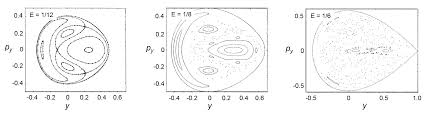
\includegraphics[scale=0.8]{images.jpg}
	\caption{Plot alla Poincarè dell'Hamiltoniana di Henon e Heiles per valori di energia crescenti}
\end{figure}
\end{exmp}
La mappa di Poincarè preserva le aree per sistemi 2-dimensionali; questo vuol dire che
\[\oint p_1\d q_1=\oint p_1' \d q_1' 			\]
Dove $(q_1,p_1)\rightarrow(q_1',p_1')$ i punti vengono mappati nel loro punto successivo (dettato dall'evoluzione temporale di $H$) nella mappa di Poincarè.\\
Per dimostrarlo facciamo uso di \ref{exmp2}; la nostra superficie di interesse ha $q_2=0=\text{cost}$ e supponiamo $H$ indipendente dal tempo: questo vuol dire che 
\[\oint H\d t=E\oint \d t =0		\]
L'esempio \ref{exmp2} dice allora che la quantità (ricordo $\d q_2=0$)
\[\oint_{\partial B}	p_1\d q_1+\oint_{\partial B} p_2\d q_2=\oint_{\partial B} p_1\d q_1=\int_B \d p_1 \d q_1	\]
è conservata (nell'ultimo passaggio si è usato il teorema di Gauss) ed è proprio l'area di una superficie nella mappa di Poincarè (presa a $q_2=0$)
\begin{exmp}[sistemi con una risonanza]
	Consideriamo l'Hamiltoniana perturbata:
	\[H=I_1+I_2-I_1^2+I_2^2+I_1I_2(\epsilon\cos(2\theta_1-2\theta_2)-3)\]
	Sicuramente si può almeno fare un cambio nelle coordinate \[\theta_1,\theta_2\rightarrow(\theta_1-\theta_2,\theta_2)\]
	per eliminare la dipendenza, dentro il coseno, da entrambe le coordinate.
	\\Il cambio delle coordinate si fa con la funzione generatrice $F_2=\vec{P}\cdot\vec{Q}(\vec{q})$, dove $\vec{Q}(\vec{q})$ indica le nuove coordinate in funzione delle vecchie. Nel nostro caso passiamo da $(\theta_i,I_i)\rightarrow(\phi,J_i)$.
	\[F_2=J_1(\theta_1-\theta_2)+J_2(\theta_2)\]
	\[I_1=\pdv{F_2}{\theta_1}=J_1\:\:\:\:\:\:I_2=\pdv{F_2}{\theta_2}=J_2-J_1=J_2-I_1\implies J_2=I_1+I_2\:\:\:\:\:\:\phi_1=\theta_1-\theta_2\:\:\:\:\:\:\phi_2=\theta_2\]
	Ora sostituiamo e si trova:
	\[H=J_2+J_2(J_2-2J_1)+J_1(J_2-J_1)(\epsilon\cos(2\phi_1)-3)=J_2+J_2^2-5J_1J_2+3J_1^2+\epsilon J_1(J_2-J_1)\cos(2\phi_1)\]
	Stavolta però $J_2$ è un integrale del moto e la variabile corrispondente ruota con velocità \[\omega_2=2J_2+1-5J_1+\epsilon J_1\cos(\phi_1)\]
	C'è un altro integrale del moto, e cioè $H$ che permette di risolvere per quadratura l'Hamiltoniana restante in $\phi_1,\theta_1$.
	\\La cosa da imparare da questo sistema è che, finchè c'è una sola risonanza, la si può eliminare con un cambio di variabili, se ce ne fossero state due, il trucco non avrebbe funzionato: è quello che succede con \ref{Henon} (lì ci sono 4 risonanze).
\end{exmp}
\subsection{Twist Map}
Un altro esempio di mappa che preserva le aree sotto evoluzione temporale: supponiamo di avere variabili azioni angolo per un sistema 2D $(\theta_1,I_1,\theta_2,I_2)$, e di mandare un punto del piano $(\theta_1,I_1)$ nel punto in cui viene mandato quando $\theta_2$ completa un periodo.
\\ Ovvero, dette $\omega_{1,2}(I_1,I_2)$ le due frequenze del sistema, prendo un punto  $(\theta_1,I_1)$ e vedo dove viene mandato dopo un periodo di $\theta_2$ ovvero dopo un tempo $t_2=\f{2	\pi}{\omega_2	}$.
\[\theta_1\xrightarrow[t_2]{} \theta_1+\omega_1 t_2=\theta_1+2\pi\f{\omega_1}{\omega_2}\]
Mentre $I_1$ resta invariato. Rappresentiamo questi punti in coordinate polari (ad esempio in figura \ref{twist}), dove $\theta$ è l'angolo e $I$ è il raggio e sia $\alpha({I_1,I_2})=\f{\omega_1}{\omega_2}(I_1,I_2)$; dato che l'energia è costante nel tempo, allora $H(I_1,I_2)=E\implies I_2=I_2(I_1,E)$, quindi si ha dipendenza solo da $I_1$. \\
Dato che questa mappa è, alla fine, una rotazione di $\theta_1$ (dipendente dal raggio), è chiaro che lascia le aree invariate. È detta twist perchè una retta a $\theta_1=\theta_0=\text{const}$ viene "piegata": parametrizzando la retta al variare di $I_1$
\[(\theta_0,I_1) \rightarrow (\theta_0+2\pi\alpha(I_1),I_1)\] 

Se $\pdv{\alpha}{I_1}>0$ la retta diventerà una specie di spirale in senso antiorario, e viceversa

\begin{figure}[h]
	\centering
	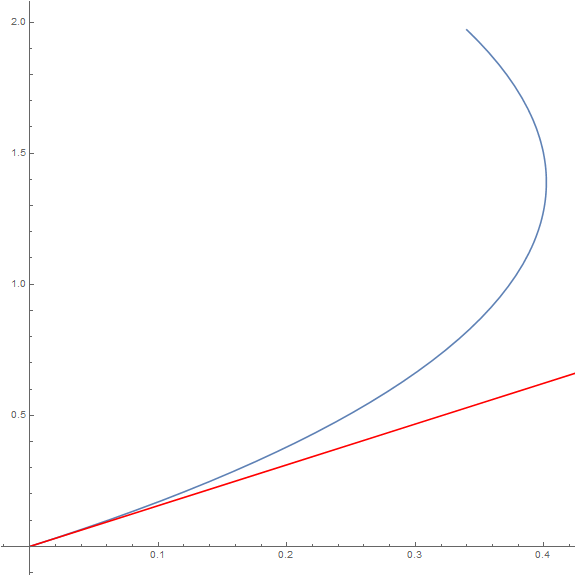
\includegraphics[scale=0.3]{twist}
\caption{Esempio di Twist map con $\pdv{\alpha}{I_1}>0$}
\label{twist}
\end{figure}
Nel caso di rapporti razionali fra le frequenze, cioè $\alpha\in\mathbb{Q}$, si avrà che un punto sarà mappato, dopo un certo numero di volte, di nuovo in sè stesso, mentre altrimenti ricoprirebbe ergodicamente tutta la circonferenza.\\
\begin{exmp}[mappa di Henon]
	Proviamo a costruire la mappa di Poincarè per un certo sistema di cui non conosciamo l'Hamiltoniana.\\Tuttavia, è nota la legge che manda un punto nel piano $q_1,p_1$ nel successivo secondo la mappa di Poincarè, quindi, prendendo un punto iniziale e reiterando il procedimento, si riescono a ricostruire le traiettorie.\\
	La mappa è la composizione di uno stiramento non lineare (ma che preserva l'area) seguito da una rotazione di un angolo fissato.\\
	Lo stiramento è il seguente:
	\[\begin{pmatrix}
	x_i\\y_i
	\end{pmatrix}\rightarrow	\begin{pmatrix}
	x_{i+1}\\y_{i+1}\end{pmatrix}=\begin{pmatrix}
	1&0\\-x_i &1
	\end{pmatrix}
	\begin{pmatrix}
	x_i\\y_i
	\end{pmatrix}	\]
	La rotazione è naturalmente del tipo:
	\[\begin{pmatrix}
	\cos(\alpha)&-\sin(\alpha)\\\sin(\alpha)&\cos(\alpha)
	\end{pmatrix}\]
	Le due operazioni lasciano entrambe le aree invariate, perchè i determinanti delle due matrici sono 1.\\
	Ad esempio, su un'ellisse, l'effetto delle due operazioni è riportato nella  figura \ref{ell}.\begin{figure}[h]
		\centering
		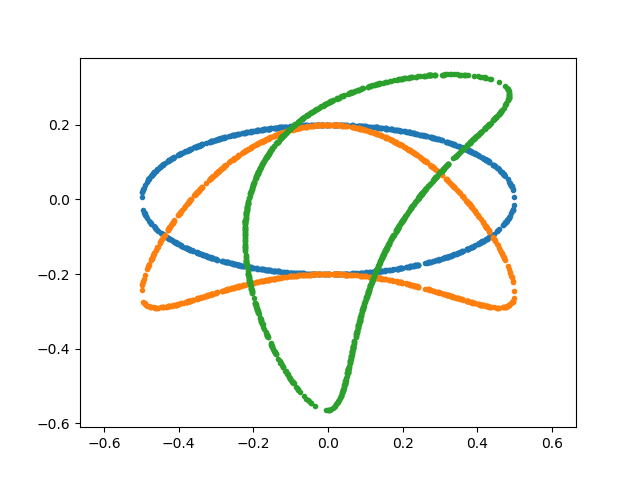
\includegraphics[scale=0.6]{ellisse}
		\caption{L'ellisse iniziale(blu) viene prima stirata (arancio) e poi ruotata (verde)}
		\label{ell}
	\end{figure}
È molto semplice scrivere un programma che, presi vari punti iniziali, li mandi nel loro successivo varie volte per vedere se si muovono su un toro invariante o in modo ergodico. Un esempio è riportato nella seguente figura \ref{epileptic} (a colori diversi corrispondono condizioni iniziali diverse).
\begin{figure}[h]
	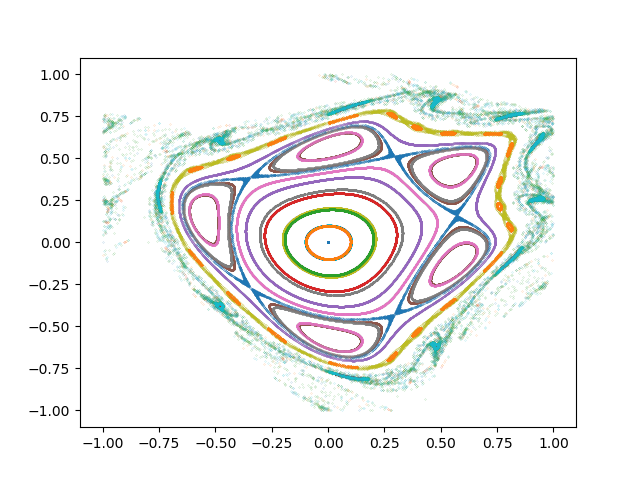
\includegraphics[scale=1.1,width=\textwidth]{epileptic}
	\caption{esempio di mappa di Poincarè secondo la legge riportata in precedenza. Si osservano vari tori invarianti, in particolare intorno al centro che è un punto fisso. La periodicità è 2 (i punti sono in $[-1,1]$) zone di caos e tori invarianti sono alternati nella regione più esterna. L'angolo $\alpha$ è scelto pari a $0.2114 \cdot2\pi$ (per riprodurre la figura riportata nel Reichl). La zona blu è di caos, ma è circondata da tori invarianti. Anche la zona giallo-verde è caotica ma all'interno presenta dei mini tori invarianti in arancione. Al centro è presente un punto fisso circondato da tori invarianti.\\ La proprietà di conservazione delle aree ci dice, ad esempio, che le aree dei tori in viola sono tutte uguali(assumendo che un toro sia mappato nel successivo, ma questo è vero se la mappa è continua, come è)}
	\label{epileptic}
\end{figure}
Al variare dell'angolo di rotazione tuttavia le figure possono cambiare di molto (il fatto che abbiamo circa 5 tori invarianti a stella che si scambiano fra loro è dovuto ad esempio al fatto che l'angolo $\alpha$ di rotazione è $\approx\f{2\pi}{5}$, credo. )
\\Questo sistema è interpretabile come una twist map perturbata: la perturbazione consiste nello stiracchiamento, mentre la rotazione è quella standard delle twist map.
\begin{figure}[h]
	\centering
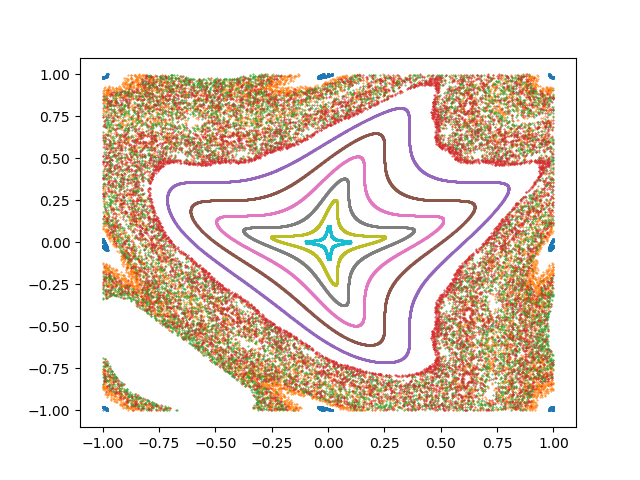
\includegraphics[scale=0.5]{attack2}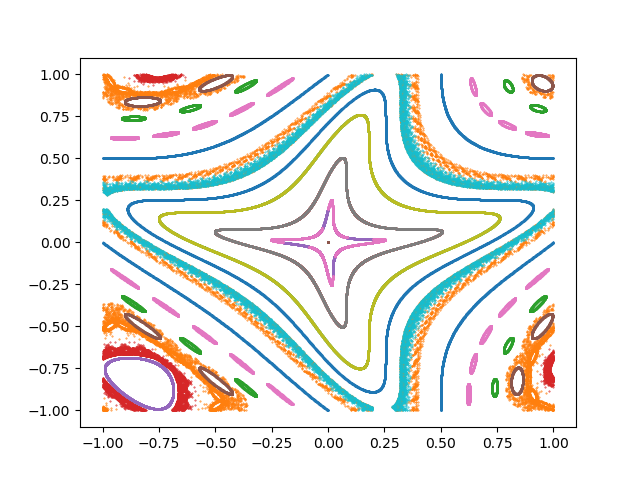
\includegraphics[scale=0.5]{attack3}
\caption{altro esempio di mappa twist per $\alpha=\f{2\pi}{4}$, nella seconda immagine il termine quadratico della trasformazione è stato soppresso per un fattore $\f{1}{2}$ il che porta ad aree di caos molto più contenute}
\end{figure}
\label{Henon2}

\end{exmp}

Vorremmo ora trovare un qualche tipo di Hamiltoniana che implichi la mappa di Henon \ref{Henon2}; ad esempio uno può provare ad integrare le equazioni del moto con intervalli discreti di tempo. \\Prendendo un'Hamiltoniana generica della forma $H=\f{p^2}{2}+V\arg{q}$, le equazioni di Hamilton sono:
\[\dot{p}=-\pdv{V}{q}\:\:\:\;\;\dot{q}=p\]
Integrando per tempi discreti si ha la mappa:
\[p_{i+1}=p_i-V'(q_i)\Delta t\quad\quad\quad	q_{i+1}=q_i+p_i\Delta t\]
Tuttavia, questa non può essere una mappa di Poincarè perchè non preserva le aree, dato che lo Jacobiano della trasformazione è:
\[J=\begin{pmatrix}
1&\Delta t\\ 
 -V''(q_i)\Delta t& 1
\end{pmatrix}\implies\det(J)=1+	V'' (\Delta t)^2	\]
Una scelta migliore consiste invece nel prendere \[p_{i+1}=p_i-V'(q_{i+1})\Delta t\]
e $q_{i+1}$ come prima.\\
In questo caso lo Jacobiano viene:
\[p_{i+1}=p_i-V'(q_i+p_i\Delta t)\implies\pdv{p_{i+1}}{q_i}=-V''(q_i+p_i\Delta t)\quad\quad\quad\pdv{p_{i+1}}{p_i}=1-\Delta t V''(q_i+p_i\Delta t)\]
Da cui il nuovo determinante è:
\[J=\begin{pmatrix}
1&\Delta t\\ 
-V''(q_{i+1})& 1- V''(q_{i+1})\Delta t
\end{pmatrix}\implies\det(J)=1	\]
Questa mappa preserva quindi le aree. In realtà lo si poteva vedere dal fatto che questa è una traformazione canonica con la \[F_4(q_{i+1},p_{i})=H \Delta t+q_{i+1}p_{i}\]

Voglio trovare un'Hamiltoniana che implichi questa evoluzione (ad intervalli di tempo fissati). Anzitutto devo fare evolvere le $q_i$ per un tempo $\Delta t=T$, e questo si può fare imponendo che \[H\arg{t,q,p}=\f{p^2}{2}\quad\quad\quad 0<t<T
\]
Avendo fatto evolvere la $q$, posso fare lo stesso con la $p$: "fisso" le $q$, imponendo che ora l'Hamiltoniana dipenda solo da $q$ per un altro intervallo $\Delta t$:
\[H=V\arg{q}\quad\quad\quad T <t< 2T	\]
Se voglio che  $T$ corrisponda anche all'intervallo di tempo in cui si ha tutta l'evoluzione (in questo caso mi era venuto $2T$), basta moltiplicare tutta l'Hamiltoniana per $2$:
\[H\arg{t,q,p}=\begin{cases}
p^2 \quad0<t<\f{T}{2}\\
2V\arg{q}\quad \f{T}{2}<t<T
\end{cases}\]
\begin{obs}
	Ci sono un mucchio di altre Hamiltoniane che hanno la stessa evoluzione, ad esempio si può scegliere di far evolvere la $p$ per un tempo $\gamma T$, $\gamma\in [0,1[$ e $q$ per un tempo $(1-\gamma)T$, nel qual caso:
	\[H\arg{t,q,p}=\begin{cases}
	\f{p^2}{2\gamma} \quad0<t<\gamma T\\
\f{	V\arg{q}}{1-\gamma}\quad (1-\gamma)T<t<T\end{cases}\]
Una scelta più carina, che permette di scrivere l'Hamiltoniana in modo più compatto, è quella di dare la botta alle $p$ in modo istantaneo (moralmente è il caso precedente facendo tendere $\gamma$ ad $1$). In tal caso la $V$ si trova a moltiplicare una $\delta$ di Dirac:
\[H=\f{p^2}{2}+\sum_{n=1}^{\infty} V\arg{q}\delta(t-nT)\]
Dove si è prolungata l'Hamiltoniana in modo periodico per tutti i tempi.\\
C'è un trucco per eliminare la dipendenza temporale esplicita dell'Hamiltoniana, aggiungendo un nuovo grado di libertà $s$ al sistema:
\[H=\f{p^2}{2}+\sum_{n=1}^{\infty} V\arg{q}\delta(s-nT)+p_s\]
dove $p_s$ è il suo momento coniugato.
\end{obs}
\begin{obs}
	\label{osservazione1}
	Ci si può chiedere cosa succede se si inverte l'ordine di evoluzione, ovvero si lascia evolvere prima $p$ e dopo $q$; nel linguaggio di prima, questo corrisponde alla mappa:\[p_{i+1}=p_i-V'(q_i)T\quad\quad\quad q_{i+1}=q_i+p_{i+1}T		\]
\end{obs}
\subsubsection{Lagrangiana discreta}
Lo schema \ref{osservazione1} riemerge anche considerando una Lagrangiana discreta del tipo:
\[\mathscr{L}_i=\f{(q_i-q_{i-1})^2}{2}-V(q_i)\]
Il principio di minima azione si traduce nel voler minimizzare:
\[S=\sum_n \mathscr{L}_n\]
\[\pdv{S}{q_i}=0\implies 2q_i-q_{i+1}-q_{i-1}-V'(q_i)=0\implies q_{i+1}=2 q_i-q_{i-1}-V'(q_i)\]
Volendo identificare l'impulso con $p_i=q_i-q_{i-1}$, si ha:
\[q_{i+1}=q_i+p_i-V'(q_i)\implies	q_{i+1}-q_i=p_{i+1}=p_i-V'(q_i)	\implies q_{i+1}=q_i+p_{i+1}	\]
Si sono riottenute le equazioni \ref{osservazione1} (con $ T=1$).\\Il fatto di evolvere prima le $p$ o le $q$ dipende dalla scelta della definizione di $p_i=q_i-q_{i-1}$ oppure $p_i=q_{i+1}-q_i$
\subsection{Standard Map}
È una mappa che evolve come la \ref{osservazione1} con il potenziale \[V\arg{q}=-\f{k}{(2\pi)^2}\cos(2\pi q)\]
Il nome standard deriva dal fatto che è molto studiata a livello teorico; una cosa interessante da notare è che alcuni tori invarianti sembrano essere fatti a trattini, in realtà zoomando sui trattini, si scopre che questi sono a loro volta piccoli tori; in realtà queste curve invarianti prendono il nome di \textbf{cantori} ed hanno proprietà in comune con il set di Cantor. Un esempio è riportato in figura \ref{cantor}
\begin{figure}[h]
	\centering
	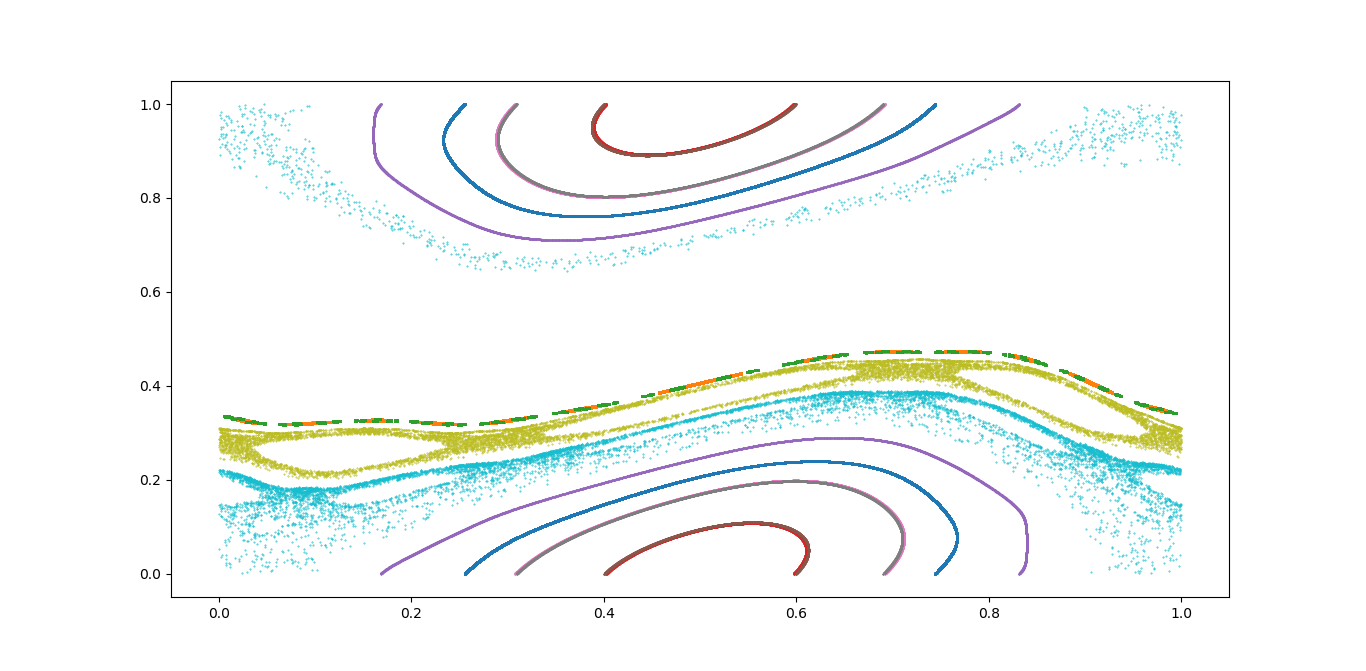
\includegraphics[scale=0.5]{util1}
	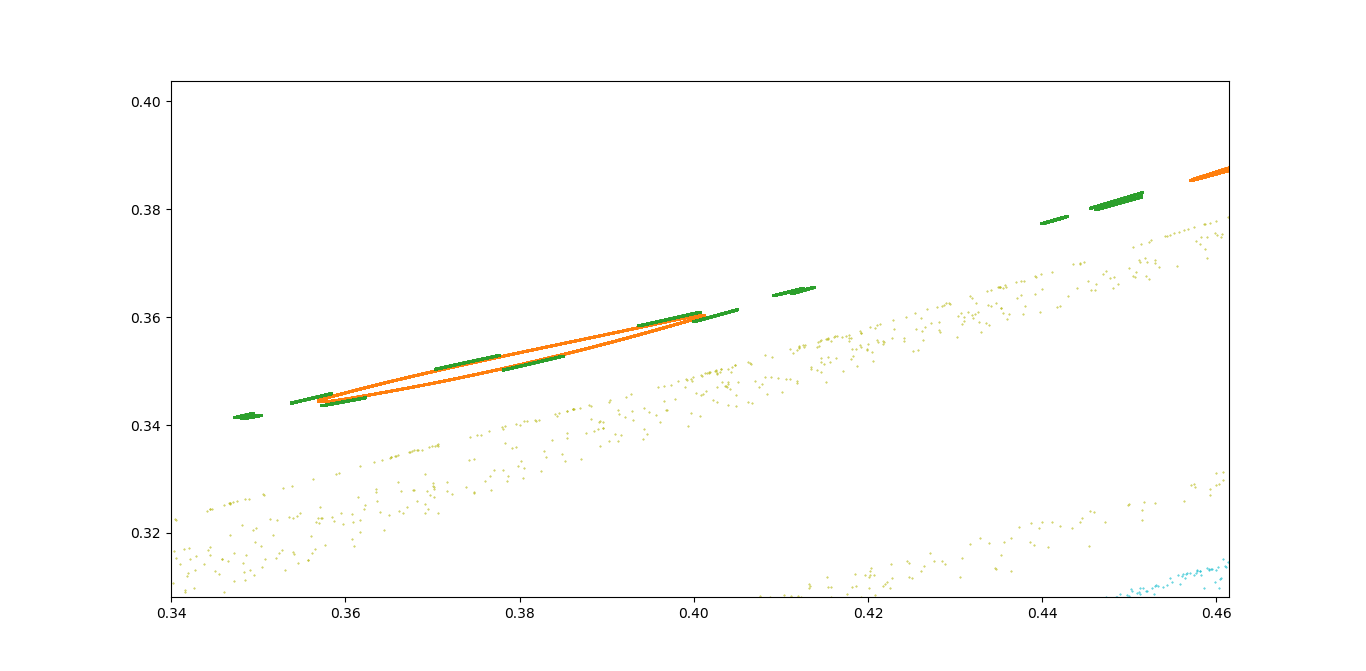
\includegraphics[scale=0.2]{util2}
	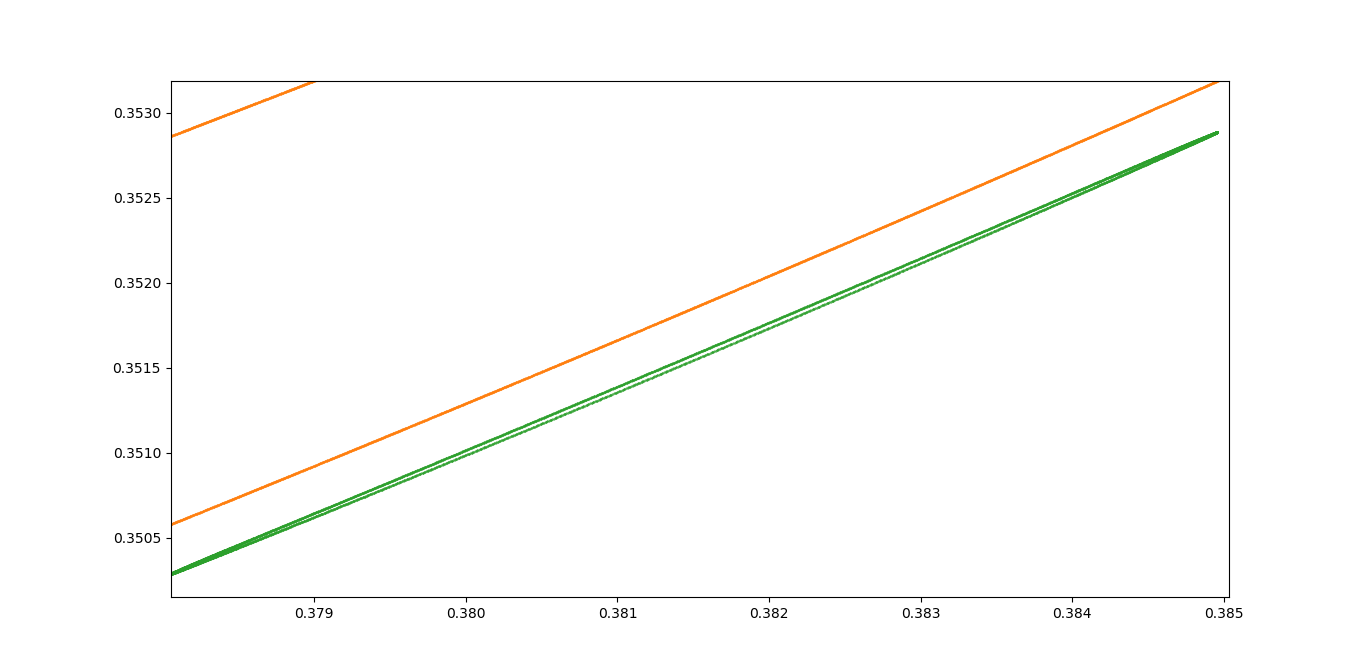
\includegraphics[scale=0.2]{util3}
	\caption{esempio di standard map con $k=1$, si può notare come le strutture verdi e arancioni al centro siano in realtà ellissi molto schiacciate, come si vede dagli zoom successivi}
	\label{cantor}
\end{figure}
\subsection{Analisi del punto fisso}
Supponiamo di avere un punto $(q,p)$ che viene mappato in sè stesso. Come nel caso \ref{expand1}, è molto semplice e fruttuoso studiare l'andamento dei punti intorno al punto fisso. A meno di traslazioni, possiamo considerare il punto fisso in $(0,0)$, ed espandere in Taylor la mappa nel suo intorno.
Sia $T$ la mappa che manda un punto nel suo successivo (in generale non è una mappa lineare);

per punti abbastanza vicini,tuttavia, basta un'espansione al prim'ordine, e la mappa sarà una matrice $\Op{M}$. Questo tipo di mappa linearizzata è detta \textbf{mappa tangente}, perchè funziona in un intorno del punto.\\
\[\Op{M}=\begin{pmatrix}
m_{11}&m_{12}\\
m_{21}& m_{22}
\end{pmatrix}\]

L'equazione agli autovalori diventa:
\[\lambda^2-(m_{11}+m_{22})\lambda+m_{11}m_{22}-m_{12}m_{21}=\lambda^2-\Tr(\Op{M})\lambda+1=0		\]
Dove si è usato il fatto che $m_{11}m_{22}-m_{12}m_{21}=\det(\Op{M})=1$ perchè la mappa è una trasformazione canonica.\\
La matrice avrà sempre $2$ autovalori diversi e quindi sarà diagonalizzabile se $\Delta\ne 0\implies |\Tr(\Op{M})|\ne2$; analizzo prima questo caso:\\
Il prodotto degli autovalori è $1$(=determinante), quindi la matrice diagonale sarà del tipo:
\[\begin{pmatrix}
\lambda&0\\
0&\f{1}{\lambda}
\end{pmatrix}\]

\begin{itemize}
\item 	Nel caso $|\tr(\Op{M})|<2$  e $|\lambda|=1$, i punti vicini ruoteranno intorno al punto fisso (punto \textbf{ellittico}).

\item Nel caso $\tr(\Op{M})>0$ (autovalori $>0$), si ha che i punti in una direzione (quella dell'autovettore corrispondente all'autovalore $>1$)si allontanano esponenzialmente, quelli nell'altra decadono esponenzialmente (come $\f{1}{\lambda^n}$); il punto è detto \textbf{iperbolico}.
\item Il caso di autovalori $<0$ ($\tr(\Op{M})<0$) è analogo al precedente; l'unica differenza è che c'è simmetria centrale ad ogni iterata a causa del segno meno: $x\rightarrow (-\lambda)^n x$; si parla \textbf{punto iperbolico con riflessione}.
\item Il caso rimasto è quello di autovalori degeneri; ci sono i casi  $\lambda=\pm1$.
In realtà non siamo certi la matrice sia diagonalizzabile; se lo è allora è $\Op{M}=\pm\unit$, quindi o i punti intorno sono tutti fissi (al prim'ordine) o vengono ogni volta specchiati dal centro.\
In generale, si può porre la matrice in forma triangolare superiore \footnote{caso particolare della forma canonica di Jordan, che forza gli elementi sulla diagonale ad essere uguali, altrimenti la matrice sarebbe diagonalizzabile} del tipo\[\begin{pmatrix}
\pm1&c\\
0&\pm 1
\end{pmatrix}\]
Supponendo di aver scelto le $q,p$ in modo tale da avere la matrice in questa forma,
si ha che questa matrice corrisponde ad una traslazione (più un'eventuale riflessione nel caso di segno meno)  di
 $q$ di una quantità $c\,p$, mentre le $p$ restano invariate; si ha quindi un'intera retta invariante (al prim'ordine) parallela all'asse delle $q$. \\Questi punti sono detti \textbf{parabolici }
\end{itemize}

\subsection{Teorema di Poincarè Birchoff}
Supponiamo di avere una twist map imperturabata: ha la forma \[\theta\rightarrow\theta+2\pi \alpha(I)\quad I\rightarrow I		\]
con $\alpha=\f{\omega_1}{\omega_2}$ nel caso derivi da una mappa di Poincarè o in generale $\alpha=\pdv{F_0}{I}$ nel caso di generica traformazione canonica ($F$ è la generatrice); supponiamo di aggiungere una piccola perturbazione, quindi $F_0\rightarrow F= F_0(I)+\epsilon F_1(I,\theta)$: per il teorema KAM, la maggior parte dei tori invarianti sopravvive (si richiede il fatto che $\pdv[2]{F_0}{I_i}{I_j}$ sia non degenere ma in 1D è scontato), tranne quelli che hanno $\alpha(I)$ razionale. Sia $T_0$ la mappa imperturbata che porta un punto nel successivo e supponiamo di scegliere un raggio $I_0$ tale che $\alpha(I_0)=\f{r}{s}$; applicando a questa circonferenza $T^s$, i suoi punti sono mandati in loro stessi. Supponiamo ora che $\alpha(I) $ sia, ad esempio, una funzione crescente. Questo vuol dire che i punti che stanno poco sopra $I_0$ saranno ruotati in senso antiorario di poco perchè \[{T_0^s}_{(I+\d I)} \theta=\theta+s\left(\f{r}{s}+\pdv{\alpha}{I}\d I\right) \gtrapprox \theta+2\pi r=\theta
\]
e viceversa quelli al di sotto di $I_0$ saranno ruotati in senso orario; inoltre le  circonferenze poco sopra e poco sotto ($I=I_0\pm\d I$), sotto l'effetto della perturbazione, avranno delle curve "vicine" invarianti per il teorema KAM, dato che non sono curve razionali.
\\Se prendo la perturbazione abbastanza piccola (rispetto a $\d I_0$), posso supporre \textbf{aggiungendo la perturbazione} che la coordinata angolare della curva più esterna $I+\d I_0$ come nel caso imperturbato aumenti  con l'applicazione di $T^s$  e viceversa per quella a $I-\d I_0$; quindi, per ogni coordinata angolare $\theta$ posso trovare l'$I(\theta)\in [I_0-\d I,I_0+\d I]$ corrispondente per cui la coordinata angolare viene mandata in sè stessa (per continuità della funzione $\alpha(I)$ perturbata). Unendo tutti questi punti  con la coordinata angolare preservata, costruisco la curva $R: (\theta,I[\theta])$. \\Applicando ad $R$ la mappa (perturbata) $T^s$ ho che la curva non viene mandata in sè stessa (anche se le coordinate angolari restano invariate, le $I$ cambiano all'ordine $\epsilon$), ma in $R'$; si ha che $R$ ed $R'$ hanno un numero pari di punti di intersezione (perchè le curve devono chiudersi: se parto da un punto di $R'$ che sta sopra $R$ , per tornarci dopo un giro di $R'$, devo risalire ogni volta che scendo sotto $R$). \\ I punti di intersezione sono dei punti fissi per $T^s$, per il fatto che la loro coordinata angolare non cambia .	\\
Ci deve sempre essere almeno un punto fisso perchè la mappa preserva le aree; se per ipotesi $R$ non si intersecasse con $R'$, si avrebbe che una delle curve dovrebbe essere contenuta nell'altra (perchè contengono una curva invariante a $I_0-\d I$, quindi hanno dei punti interni in comune), ma allora una avrebbe aree più piccola dell'altra, assurdo.\\

Inoltre i punti devono anche essere multipli di $s$ perchè, preso un punto fisso $x$ e applicandoci $T^t$ con $t<s$, non lo mando in sè stesso visto che all'ordine $0$ i punti vengono ruotati di $2\pi \f{t r}{s}$ (che non è un multiplo intero di $2\pi$). Tuttavia 
\[T^t x=T^t T^s x= T^s T^t x		\]
quindi anche $T^tx$ è un punto fisso. Se ne deduce che ci sono $2ks$ punti fissi, $k\in\mathbb{N}$ (in teoria così sto dimostrando che sono almeno $k s$, ma la parte restante del teorema implica che  $k$ deve essere pari, visto che li  posso dividere in due famiglie grandi uguali di punti stabili e instabili).\\
Ora voglio far vedere che questi punti sono, alternativamente, stabili e instabili.
\begin{figure}[h]
	\centering
	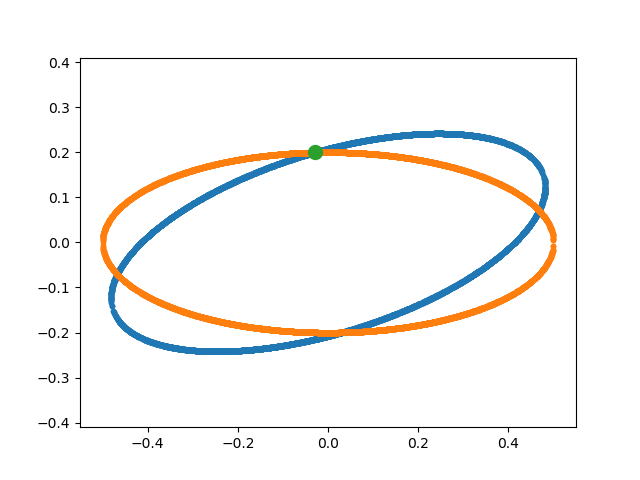
\includegraphics[scale=0.5]{exmp}
	\caption{esempio di figura di $R$ (in arancio) ed $R'$ in blu}
	\label{yourmother}
\end{figure}
Concentriamoci sul punto di intersezione in verde in figura \ref{yourmother}; dopo l'applicazione della mappa $T^s$, i punti a destra dell'intersezione salgono su $R'$, ma se sono sopra $R$, vuol dire che dopo l'applicazione di $T^s$ ruoteranno in senso antiorario\footnote{si è presa per ipotesi $\alpha(I)$ crescente nell'intorno della nostra curva, quindi all'aumentare di $I$ (il raggio), l'angolo di rotazione aumenta(=ruotare in senso antiorario) dopo l'applicazione di $T^s$}, e la loro coordinata angolare aumenterà, tendendoli a riavvicinare al punto di intesezione in verde: il punto è di tipo ellittico (stabile). Viceversa il punto di intersezione successivo, che immagino trovarsi a $\theta=\theta_0$, ha che i punti con $\theta<\theta_0$ "scendono" (il loro raggio diminuisce); dato che sono scesi dentro $R$, vuol dire che altre applicazioni di $T^s$ li allontaneranno ancora di più (ruotano in senso orario diminuendo ancora di più $\theta$ e quindi allontanandosi da $\theta_0$): si ha un punto iperbolico instabile . 
\\Ripetendo il ragionamento, si dimostra che ci sono alternativamente punti stabili ed instabili. Inoltre $T$ mappa un punto di equilibrio stabile in un punto stabile. Infatti, preso $x$ vicino ad $x_0$ che è stabile, si ha che $T^s x$ è vicino ad $x$; se $T$ è continua $T^t T^s x=T^s T^t x$ è vicino a $T^t x$ , quindi i punti intorno a $T^t x$ restano vicini sotto applicazione di $T^s$, questo vuol dire che i punti del tipo $T^tx_0$ sono tutti stabili (e sono $s$ punti). Dato che per ogni punto stabile ce ne deve essere uno instabile, ci sono $2ks$ punti fissi.
\\ In definitiva, il nostro toro razionale di partenza, sotto $T^s$, si spezza in $ks$ punti ellittici (con intorno dei tori invarianti) ed altrettante zone caotiche intorno ai punti fissi iperbolici\footnote{Si intende tori invarianti rispetto a $T^s$, non  $T$, il cui toro invariante è $I=const=I_0$ e si frantuma sotto la perturbazione, avendo per ipotesi una $\alpha=\f{\omega_1}{\omega_2}$ razionale}.
\\Ma fra questi tori invarianti ci saranno ancora dei tori razionali che si spezzeranno a loro volta in altri tori (rispetto alla mappa $({T^s})^q$, visto che stavolta si parte da $T^s$), e così via, creando una struttura auto-similare.\\
Ad ogni spezzettamento dovuto al teorema si ha un passaggio dall'applicare $T$ all'applicare $T^s$, quindi la struttura frattale si vede facendo effettivamente infinite reiterazioni della mappa (altrimenti si vedrebbe ovunque nelle simulazioni numeriche, dato che le frequenze sono tutte razionali, essendo i punti discreti.).
\subsection{Punti iperbolici}
Nell'intorno di un punto iperbolico instabile si ha un comportamento molto peculiare; anzitutto si ha che i due autovalori nell'intorno sono $\lambda\econg\f{1}{\lambda}$; il comportamento dei punti nelle due direzioni corrispondenti è:
\[x_n=x_o \lambda^n\quad\text{oppure} \quad x_n =x_0\left({\f{1}{\lambda}}\right)^n		\]
supponendo $|\lambda|>1$, la soluzione stabile è quella lungo l'autovettore di $\f{1}{\lambda}$. Possiamo prolungare le curve che partono dal punto fisso nelle direzioni dei due autovalori: chiamiamole $H_0^+$ per la traiettoria stabile e $H_0^-$ per quella instabile.
\begin{obs}
Bisogna fare qui due importanti precisazioni; (spero di averla imbroccata giusta, però) le traiettorie di cui stiamo parlando, del tipo $H_0^{\pm}$ non sarebbero di base ben definite se non grazie al fatto che partiamo da un punto fisso, e, iterando $T$ su un segmento infinitesimo che parte da lì nella direzione di partenza desiderata, si riesce a costruire una curva (varietà 1D), questo perchè i punti vengono sempre mappati nell'intorno del punto fisso, quindi, si riesce ad ogni mappa a prolungare la curva. Se invece la traformazione fosse, ad esempio, una rotazione di $\f{\pi}{2}$ (la butto lì), un segmentino sarebbe mappato a caso da un'altra parte e non sarebbe connesso col pezzo di partenza.\\Seconda precisazione: qui come mappa non stiamo necessariamente prendendo $T$, ma in generale possiamo decidere di mappare secondo $T^3$ o altro; ad ogni scelta corrisponderanno traiettorie diverse ( cambiano i punti fissi). 


\end{obs}

Queste due traiettorie $H_0^{\pm}$ possono poi, ad esempio intersecarsi; un esempio semplice è quello del pendolo, per il particolare valore dell'energia $E=mgl$. L'Hamiltoniana è:

\[H=\f{p^2}{2m}-mgl\cos(x)=mgl		\]

Da cui :
\[p=m\sqrt{2lg}\sqrt{1+\cos(x)}=\pm2m\sqrt{lg}	\cos(\f{x}{2})		\]

\begin{figure}[h]
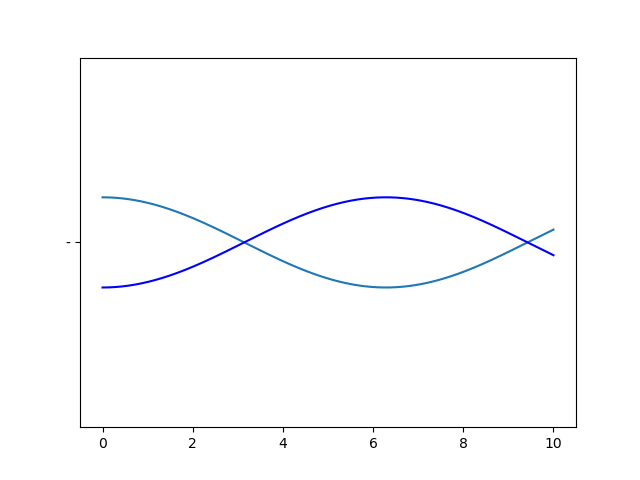
\includegraphics[scale=0.5]{Figure_1.png}
\caption{linee su cui si svolge il moto nel pendolo semplice. Le intersezioni sono punti iperbolici e le due varietà si intersecano più volte}
\end{figure}


Si introduce una nomenclatura per indicare le varie tipologie di intersezioni.
\begin{itemize}
	
\item 	Si può avere un' \textbf{orbita omoclina} quando $H_0^+$ e $H_0^-$ non sono altro che le estremità di un "nodo" di una singola curva che si auto-interseca.
	\item Si chiamano invece \textbf{punti omoclini} le intersezioni di due varietà che provengono dalla stessa \textbf{famiglia}, che è un modo per dire che sono generati dalla mappa $T^s$ con $s$ uguale per le due traiettorie.
	\item Il caso uguale al precedente, ma con le due traiettorie generate da $T^s_1$ e $T^s_2$ diversi, dà origine a \textbf{punti eteroclini}.
	
\end{itemize}
Ora supponiamo di avere un punto omoclino $X$, intersezione di $H_0^\pm$ : mappando questo punto con la $T$ che genera le due curve si ha, dato che il punto appartiene sia ad $H_0^+$ che ad $H_0^-$, che anche la sua immagine $TX$ deve appartenere ad entrambe le curve. \\Inoltre, la curva stabile $H_0^+$ si avvicina, ad ogni interazione, al punto iperbolico $X_0$, questo vuol dire che $TX$ si avvicinerà ad $X_0$ (questo forza la sua mappa a stare dal lato "giusto" della curva), un esempio di questo andamento è riportato in figura \ref{osc}.

\begin{figure}[h]
\centering

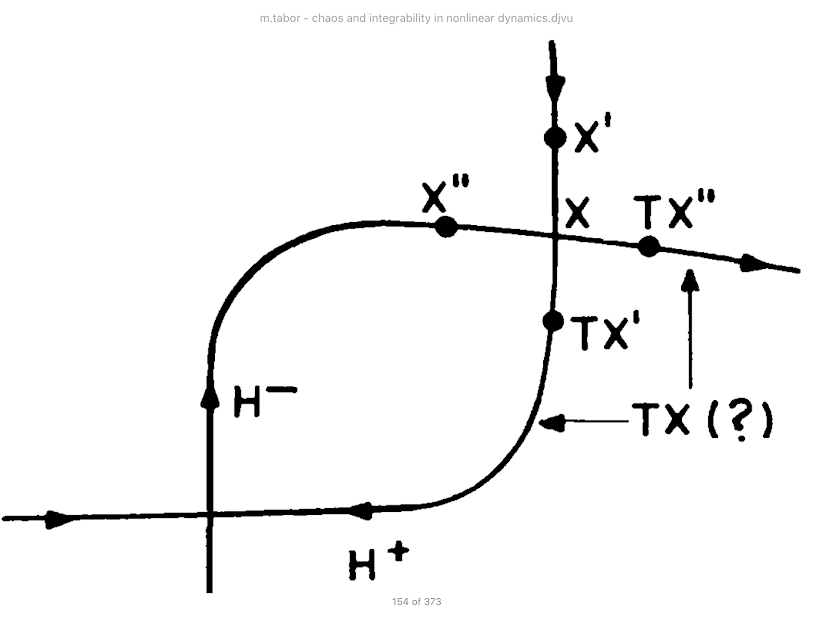
\includegraphics[scale=0.2]{Tabor1}
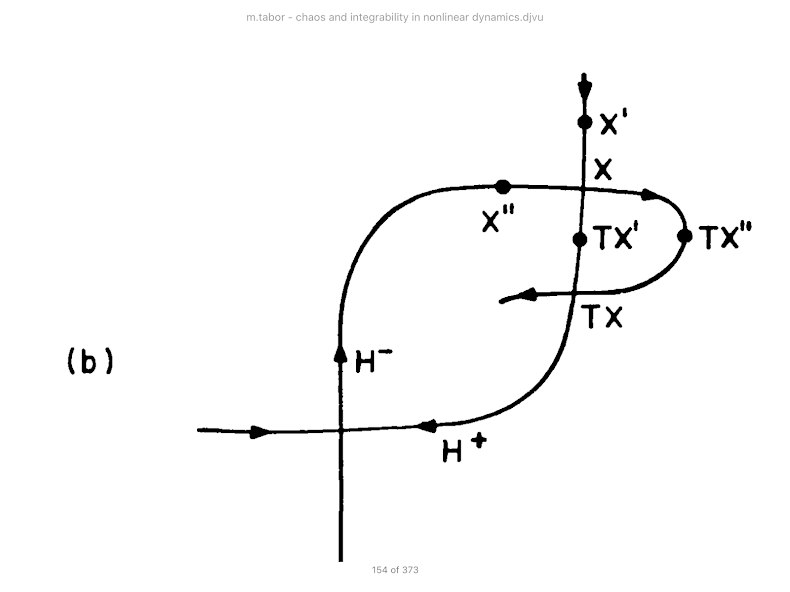
\includegraphics[scale=0.26]{Tabor2}
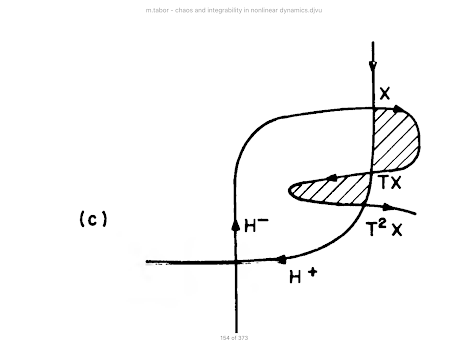
\includegraphics[scale=0.5]{Tabor3}

\caption{esempio di mappatura di punti omoclini in successive intersezioni delle due curve, immagine presa dal Tabor, "chaos and integrability in nonlinear dynamics"}
\label{osc}
\end{figure}
 Continuando a mappare con la $T$ le intersezioni si ha che ci si avvicina sempre di più ad $X_0$ e di conseguenza la distanza fra le $T^n X$ si riduce sempre di più (ricordo che, dato che i punti stanno anche su $H_0^+$, si devono avvicinare al punto come $\f{1}{\lambda^n}$). \\
Inoltre, considerando il percorso chiuso $\Op{C}_n$ creato dai pezzi di $H_0^\pm$ compresi fra $T^n X$ e $T^{n+1}X$, si ha che viene mappato dal percorso successivo dalla $T$, perchè i suoi estremi sono mappati negli estremi  del circoletto successivo per ipotesi.
\[T \,\Op{C}_n=\Op{C}_{n+1}\] 
ma l'area racchiusa da $\Op{C}_n$ deve essere la stessa per ogni $n$ per il teorema di Liouville, questo vuol dire che le oscillazioni di $H_0^-$ diventano sempre più intense. Si genera alla fine una figura del tipo \ref{osc2}.
\begin{figure}[h]
	\centering
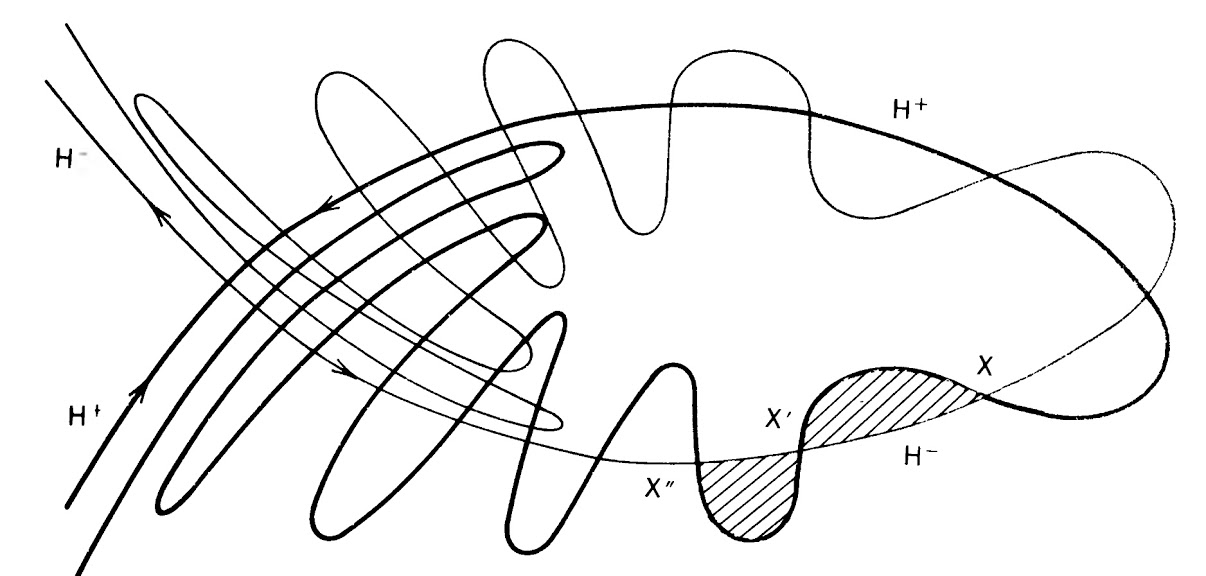
\includegraphics[scale=0.3]{Tabor4}
\caption{esempio dell'evoluzione di un punto omoclino}
\label{osc2}

\end{figure}


È chiaro che un sistema del genere si sfascia alla minima perturbazione ed è estremamente instabile a seconda delle condizioni  iniziali: è un sistema caotico.
\\Un'ultima notazione: il tabor segnala che questa struttura ad oscillazioni sempre più fitte ed intense prende il noma di \textbf{Tendril} e si ottiene continuando a mappare un segmento con la mappa $T$ vicino ad  un punto iperbolico (cioè a disegnare $H^-$); tentando di fare la stessa cosa vicino un punto ellittico porta ad una roba del tipo quella riportata in \ref{whorl}, questa struttura prende il nome di \textbf{whorl}.
\begin{figure}[h]
	\centering
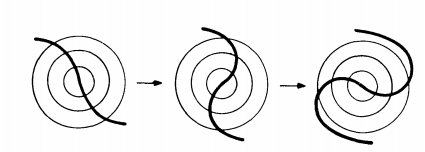
\includegraphics[scale=0.6]{whorl}\caption{Iterate di un segmento vicino un punto ellittico; i cerchi sono le curve invarianti}\label{whorl}\end{figure}
\\Infine, riguardo ai punti eteroclini, questi si manifestano quando il caos è gia parecchio sviluppato e si sono rotti anche i tori più irrazionali, dato che ora il sistema può passare facilmente da curve invarianti di un certo $T^n$ a quelle con un altro esponente, rimescolando di molto tutti i punti.


\section{Esponenti di Lyapunov}
Sono dei numeretti che identificano il livello di "caoticità" del sistema; in particolare, ci si aspetta che per un sistema caotico due punti "vicini" si allontanino rapidamente nel tempo.
\\Naturalmente non si possono allontanare in eterno, essendo il sistema (sperabilmente) limitato.
Presa una mappa $T$ tale che 
\[\pos^{i+1}=T\pos^i=\vec{F}(\pos^i)\]
l'andamento di punti vicini distanti $\delta \pos^i$ si ottiene facendo la variazione rispetto $\pos$ dell'equazione precendente;
\[\delta\pos^{i+1}=\left.\pdv{\vec{F}}{x_j}\right|_{\vec{x}^i}{\delta x^i_j}	\]
in pratica si guarda la mappa tangente calcolata in $\pos^i$. Se si assume che la distanza fra punti vicini aumenti esponenzialmente, del tipo $|\delta x^i|=e^{\sigma i}  |\delta x^0|$, allora si ha che il parametro di allontanamento $\sigma$ è pari a :
\[\sigma=\ln\left(\lim_{i\rightarrow\infty}  \left(\f{\delta x^i}{\delta x^0}\right)^{\f{1}{i}}\right)	\]
Se invece dell'andamento della distanza, si vuole guardare il caos nelle varie direzioni, si guardano i vari autovalori della matrice che determina l'allontanamento.
\\Detta $M(\pos)$ la mappa tangente calcolata nel punto $\pos$, si ha che \[\delta \pos^n=\prod_{i=0}^{n-1} \Op{M}(\pos^i)  \delta \pos^0\]
Diagonalizzando la matrice $\prod_{i=0}^{n-1} \Op{M}(\pos^i) $ ci si aspetta di trovare come autovalori gli stretching nelle varie direzioni $\lambda_j^n$ elevati al numero di interazioni; volendo l'allontanamento medio si ha che gli esponenti di Lyapunov sono il logaritmo degli autovalori della seguente matrice ($\pos_i=T^i \pos_0$):
\[\lim_{n\rightarrow \infty}	\left(\prod_{i=0}^{n-1} \Op{M}(\pos^i) 	\right)^{\f{1}{n}}	\]

oppure gli autovalori della matrice
\[\lim_{n\rightarrow\infty}\f{1}{n}\sum_{i=0}^{n-1}\ln\left( \Op{M}(\pos^i) 	\right))	\]
il che rende più chiaro il processo di media sulle $n$ interazioni(l'ordine del processo "faccio il logaritmo"$\ra$"calcolo gli autovalori" o viceversa chiaramente non conta).
\\ Questo limite non dovrebbe dipendere dalla scelta delle condizioni iniziali, eccetto che per un set di condizioni iniziali che ha misura nulla.
Intuitivamente questo si giustifica col fatto che sistemi caotici (cioè che hanno esponenti di Lyapunov $\ne 0$) visitano più o meno tutto lo spazio delle fasi, eccetto che "piccole" zone

\begin{exmp}
	Calcolo l'esponente di Lyapunov con la mappa 1D (con periodo $1$, perchè vogliamo le $x$ limitate):
	\[x_{i+1}=2x_i\]
	La mappa tangente è uguale alla mappa vera e propria (perchè questa è lineare), e la matrice è semplicemente la moltiplicazione per $2$.
	\[\f{1}{n}		\sum_{i=0}^{n-1} \ln(2)=\ln(2)	\]
	Questo è l'esponente di Lyapunov
	
	
	
\end{exmp}




Assumiamo ora una dinamica continua:
\[\dv{\pos}{t}=\vec{f}(\pos)	\]
Volendo guardare punti vicini, si fa sempre la mappa tangente calcolata sulla traiettoria:
\[\dv{\delta x_i}{t}=\left.{\pdv{{f}_i}{x_j}}\right|_{\pos(t)}{\delta x_j}=\Op{M}(\vec{x}(t)) \delta \pos				\]

Rispetto a prima, però, vogliamo fare step infinitesimi. Dato che l'equazione per l'evoluzione temporale è lineare, posso definire una matrice $\Lambda$ per l'evoluzione temporale:
\[\delta \pos(t)=\Lambda(t) \delta \pos(0)		\]
Dove naturalmente $\Lambda(0)=\unit$.
Inserendo tutto nell'equazione per l'evoluzione temporale, si trova:
\[\dot{\Lambda}=\Op{M}(\vec{x}(t))\Lambda			\]
Quindi gli esponenti di Lyapunov saranno gli autovalori di:
\[\lim_{t\rightarrow\infty}	\f{\ln(\Lambda(t))}{t}		\]


Esistono particolari simmetrie per quanto riguarda gli esponenti di Lyapunov, nel caso si guardi ad un'evoluzione Hamiltoniana.
\begin{itemize}
	\item  \[\sum_i \sigma_i=0\]
	Questo segue dal fatto che la matrice $\Lambda$ che manda $\delta \vec{z}(0)\rightarrow\delta \vec{z}(t)$ è lo Jacobiano $J(t)=\pdv{\vec{z}(t)}{\vec{z}(0)}$ dell'evoluzione temporale, che è una trasformazione canonica, quindi ha determinante 1:
	\[1=\det(J)=\prod_{i=0}^{2n} \lambda_i\sim\exp(\sum_{i=0}^{2n} \sigma_i t  )\implies\sum_{i=0}^{2n} \sigma_i=0 		\]
	\item  gli esponenti di Lyapunov, a coppie, hanno la proprietà che :
		\[\sigma_i=-\sigma_j\]
		Questo discende dal Teorema \ref{Sim} ricordando che $\lambda_i\sim e^{\sigma_it}$
	\item  Supponendo l'Hamiltoniana indipendente dal tempo, si ha che c'è almeno un integrale del moto, e quindi una direzione in cui la $\vec{z}$ non si espande (presi due punti distanti $\delta \vec{z}$ restano sui due rispettivi tori invarianti,quindi non si possono allontanare troppo). Di conseguenza c'è almeno un $\sigma_i=0$ e, per la proprietà precedente, ce ne sono almeno 2.
\end{itemize}

Il calcolo di questi esponenti è comunque molto complesso (bisogna risolvere un'equazione differenziale con le matrici e  diagonalizzare il risultato), oppure risolvere il moto, cosa non pensabile per sistemi caotici, che sono il caso in cui gli esponenti sono diversi da $0$.\\ Esistono comunque algoritmi semplici per trovare il massimo degli autovalori. Intuitivamente, se $\Lambda$ diverge esponenzialmente, il suo autovalore che esplode più in fretta dominerà la matrice (gli altri saranno trascurabili), e la matrice sarà quasi  un proiettore sull'autovalore corrispondente.
\\ L'algoritmo corrispondente (Bennettin et al.)è il seguente: parto con un vettore $\delta\vec{z}_0$ iniziale e ad ogni step lo faccio evolvere per un tempo $\tau$. A questo punto definisco 
\[\delta \vec{z}_1=\f{\delta\vec{z}_0(\tau)}{|\delta\vec{z}_0|}\]
che poi faccio evolvere per un tempo $\tau$, ottenendo $\delta \vec{z}_2$, e così via per costruire una sequenza.
L'idea è che ad ogni step il mio vettore iniziale viene proiettato sempre di più verso la direzione di massima dilatazione, idealmente si dovrebbe avere che $e^{\sigma\tau}=\f{|\delta \vec{z}_i(\tau)|}{|\delta \vec{z}_i(0)|}=|\delta \vec{z}_i(\tau)|$, ricordando che ad ogni step i vettori partono normalizzati.\\ Quindi facendo la media di una dilatazione ad ogni step, ottengo la dilatazione massima:
\[\sigma=\sum_{i=0}^{N-1}\f{1}{\tau N }\ln \left( {|\delta \vec{z}_i(\tau)|}	\right)	\]
Le seguenti proprietà sono state dimostrate formalmente:
\begin{itemize}

\item Esiste il limite\[
\sum_{i=0}^{N-1}\f{1}{\tau N }\ln \left( {|\delta \vec{z}_i(\tau)|}	\right)\]

\item Il limite è indipendente dalla scelta di $\tau$
\item se il punto iniziale è scelto nella zona non caotica (con un qualche integrale del moto, cioè) dello spazio delle fasi, il limite è 0
\item  se il punto iniziale è scelto nella zona caotica dello spazio delle fasi, il limite è $>0$ ed indipendente dal punto iniziale

\end{itemize}
\section{Entropia di Kolmogorov-Sinai}
La definizione è un po' complicata, quindi prima definisco:
\begin{defn}[Partizione]
	Dato lo spazio delle fasi $\Op{S}$, si definisce una partizione $Q$, come l'insieme di dei sottoinsiemi $Q_i$ di $\Op{S}$
	tali che 
	\[\bigcup_i  Q_i=\Op{S}		\]
	\[\forall(i,j):\quad	Q_i\cap Q_j=\emptyset	\]
	
\end{defn}
Supponiamo ora di avere una mappa $T$ che manda un punto nel successivo.
\\Fatta la partizione, si immagina, dato un punto iniziale $x$ che rappresenta il sistema, di poter misurare, ad ogni iterata di una mappa $T$ che definisce la dinamica,
in quale delle $Q_i$ si trova $x$ nello step $n$-esimo.
Supponendo ad esempio di misurare inizialmente $x$ in $Q_j$ e  $Tx$ in $Q_i$, si scopre che la nostra $x$ iniziale si trova in effetti in un punto contenuto in $Q_j\cap T^{-1} Q_i$ ($T^{-1} Q_i$  è la controimmagine di $Q_i$, ovvero l'insieme dei punti che vengono mandati in $Q_i$ dalla $T$).
Quindi, andando a vedere il passato ed il presente, è come se avessimo fatto una partizione  più fine con elementi $Q^2$ contenente come elementi \[Q^2_{ij}=Q_i\cap T^{-1} Q_j\] Andando a fare altre misure,  dopo l'applicazione di $T^2,T^3,\ldots$, si costruisce una partizione ancora più fine $Q^3=\{Q_i\cap T^{-1} Q_j\cap T^{-2} Q_k\}		$, e così via.
\\Data una partizione $Q$, si definisce la sua entropia:
\[S(Q)=-\sum_i	\mu(Q_i)\ln(\mu (Q_i))	\]
Dove \[\mu(Q_i)=\int_{Q_i} \d \mu		\]
è la misura del sottoinsieme dello spazio delle fasi.
A questo punto, data una partizione iniziale $Q$, si definisce la sua entropia di Kolmogorov-Sinai, la quantità:
\[S_{KS}(Q)=\lim_{n\rightarrow\infty}	\f{S(Q^n)}{n}	\]
Dove il $Q^n$ indica la partizione costruita nel modo indicato sopra con $n$ steps.\\
Questa quantità dice essenzialmente la minima entropia (cioè la massima informazione) che si riesce ad estrarre dal sistema data una partizione di misura.\\
La "vera" entropia del nostro sistema dinamico è il sup delle entropie di tutte le partizioni, rispetto alla scelta della partizione iniziale:
\[S_{KS}=\sup_{Q} S_{KS}(Q)		\]
La presenza di questo $\sup$ rende l'entropia praticamente impossibile da calcolare in pratica, se non fosse per un teorema che dice che il $\sup$ delle possibili partizioni è raggiunto se, come partizione iniziale, si prende una generatrice.

\begin{defn}[generatrice]
	È una particolare partizione $G$ dello spazio delle fasi, tale per cui andando a vedere in quale $G_i$ si trova $T^{n} x$, per ogni $n$, si riesce a risalire in modo univoco ad $x$. \\Detto in altri termini, data $x$, la sequenza di "indici" $\{w_n\}$ che indica in quale elemento della partizione $G$ si trova $x$ allo step $T^{n}$ è:
	\[w(x)=\{w_n\in I|n\in \mathbb{Z}, T^{n} x\in G_{w_n}\}\]
	Allora la partizione $G$ è detta generatrice se esiste una relazione biunivoca $x\leftrightarrow w(x)$, ovvero se dalla sua sequenza si riesce a risalire ad $x$.
	
\end{defn}

\begin{exmp}[Baker's map]
Consideriamo la seguente mappa, per $q,p\in [0,1]^2$:
\[T(q,p)=\begin{cases}
\left(2q,\f{p}{2}\right)\quad q\in[0,\f{1}{2}]\\

\left(2q-1,\f{p+1}{2}\right)\quad q\in[\f{1}{2},1]\\


\end{cases}
\]

La mappa consiste sostanzialmente nel dividere in due fettine il quadrato, schiacciarle, e riattaccarle una sopra l'altra (è per questo rimescolamento che si chiama mappa del panettiere).\\
Si vuole calcolare l'entropia $KS$ di questa mappa.
\\Bisogna fare anzitutto un'osservazione: data una partizione $Q$, che spezzetta lo spazio delle fasi in $N$ regioni con misura $\mu(Q_i)$ (la cui somma è fissata), la quantità
\[\sum_i \mu(Q_i)\ln(\mu(Q_i))\]
è massima se $\mu(Q_i)=\f{\mu(Q)}{N}$ cioè se tutte le regioni hanno area uguale.
\\Ciò detto, prendo come partizione iniziale \[Q=\{[0,\f{1}{2}]\times[0,1],[\f{1}{2},1]\times[0,1]\}\]
che divide il piano lungo $q=\f{1}{2}$ in due strisce uguali. Andiamo a vedere $Q^2=\{Q_i\cap T^{-1} Q_j		\}$: questa partizione divide anche le $p$ a metà.
Continuando il processo, si vede che ad ogni partizione, le $p$ vengono divise in pezzetti sempre più piccoli (dimezzati ad ogni interazione).
\begin{figure}[h]
	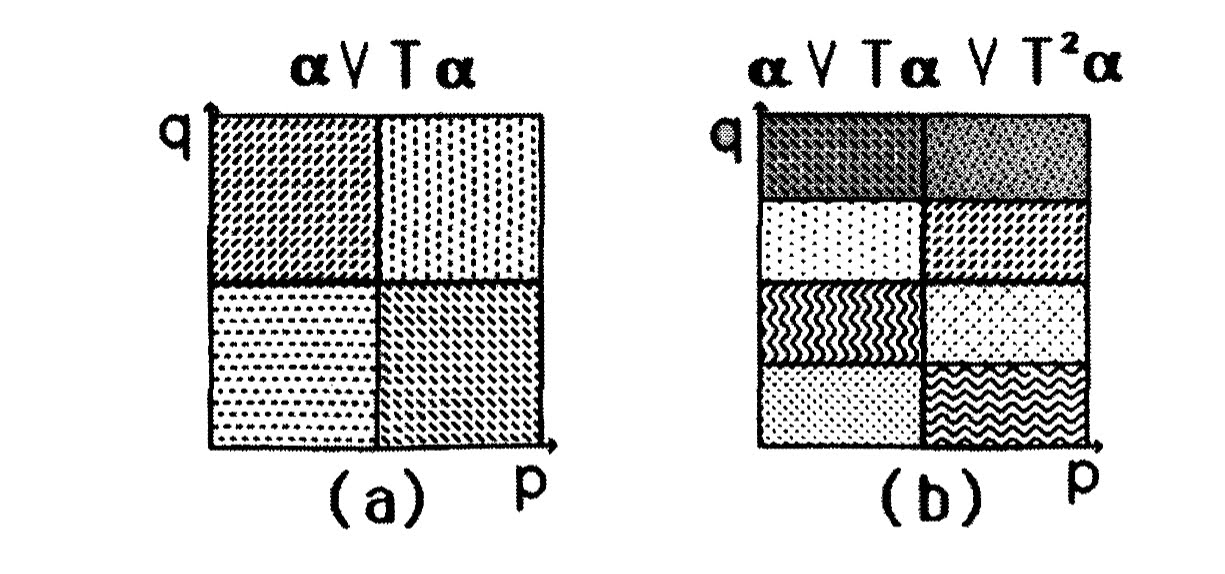
\includegraphics[scale=0.3]{baker}
	\caption{evoluzione della partizione alla prima e seconda iterazione della $T$}
	\label{Baker}
\end{figure}
Quindi, ad ogni iterazione, lo spazio delle fasi è diviso in $2^n$ regioni di area uguale. Grazie all'osservazione precedente, in questo modo si massimizza l'entropia, quindi si ottiene il $\sup$ della formula di $S_{KS}$.
\[S_{KS}=\lim_{n\rightarrow\infty}	-\f{1}{n}\sum_{i=1}^{2^n} \f{1}{2^n} \ln(\f{1}{2^n})	=\lim_{n\rightarrow\infty}	\f{1}{n}\sum_{i=1}^{2^n} n\f{1}{2^n} \ln(2)	=\ln(2)\lim_{n\rightarrow\infty}	 \sum_{i=1}^{2^n}\f{1}{2^n}	=\ln(2)\]
Questa quantità è anche pari agli esponenti di Lyapunov, dato che c'è uno stretching di $2$ lungo le $q$, quindi i due esponenti saranno \[\sigma_{1,2}=\pm\ln(2)\]

\end{exmp}

\section{Chaos Globale}
\subsection{Distanza di Melnikov}

Serve a capire se le due varietà, quella stabile ed instabile, che partono da un punto iperbolico, si intersecano o meno (nel qual caso si avrebbe Chaos).
Si parte da un'orbita omoclina, che si chiude in sè stessa. Questa si rompe nel caso di una perturbazione \[H=H_0+\epsilon V\]
che causa la separazione di $H_0^{\pm}$ in due varietà. Se queste due varietà si intersecano creando un punto omoclino, si genera chaos, come visto nella sezione precedente. Si definisce la \textbf{distanza di Melnikov} la distanza fra le due varietà rotte in caso di piccola perturbazione (prende il nome del tizio il quale per primo trovò un modo analitico di calcolarla).
\\Si parte da un punto $\vec{r}_0(0)$ sulla traiettoria imperturbata. Si ha quindi che $\vec{r}_0(\infty)$ tende ad avvicinarsi al punto iperbolico da cui si generano le due varietà, lungo $H_0^+$, mentre $\vec{r}_0(-\infty)$ tende sempre al punto iperbolico, ma dal "lato" di $H_0^-$, da cui il sistema è "scappato".
\\In presenza della perturbazione la varietà $H_0^\pm$ si rompe in $H^+$ e in $H^-$; queste all'ordine più basso mantengono la stessa forma\footnote{è difficile da spiegare senza un disegno, diciamo che è come se ci fossero due copie del "nodo" (dell'orbita omoclina, un esempio di figura è \ref{Duffin}) che sono leggermente spostate una rispetto all'altra a causa della perturbazione, altrimenti si sovrapporrebbero}, quindi per misurarne la distanza  basta prendere la proiezione su due punti appertenente uno ad $H^+$ ed uno ad $H^-$ lungo la direzione perpendicolare (che è comune, visto che all'ordine 0 la "forma" delle varietà è invariata ) alla traiettoria.
\\Il vettore (non normalizzato) tangente alla traiettoria, in un punto $\vec{r}_0$ è, supponendo un sistema Hamiltoniano $(q,p) $:
\[\vec{t}\propto\dot{\vec{r}}_0=\begin{pmatrix}
\pdv{H_0}{p}&
-\pdv{H_0}{q}
\end{pmatrix}	\]
Da cui il vettore perpendicolare è \[\vec{n}\propto	\begin{pmatrix}
\pdv{H_0}{q}&
\pdv{H_0}{p}
\end{pmatrix}	=\vec{\nabla}H_0\]
(la cosa era ovvia perchè il moto si svolge lungo $H$ costante, quindi il suo gradiente è ortogonale alla traiettoria).
\\Il fatto che non guardo alla normalizzazione di $\vec{n}$ mi farà avere il risultato finale sbagliato di un certo fattore; io però sono interessato ai punti di intersezione, dove cioè la distanza vale $D=0$, per quello posso ignorare la normalizzazione.\\
Adesso bisogna vedere dove viene mandato $\vec{r}_0$ quando si spezza nei due punti sulle due diverse varietà $H^{pm}$ (in seguito alla perturbazione).
In particolare, sia $\Delta \vec{r}^+(t)=\vec{r}^+(t)-\vec{r}_0(t)$ la distanza dei punti della nuova varietà stabile perturbata da quelli della vecchia orbita omoclina, e analogamente per $\Delta \vec{r}^-(t)$ rispetto alla varietà instabile.
\[\Delta\dot{\vec{r}}^+(t)=\left.\begin{pmatrix}
\pdv{H}{p}&
-\pdv{H}{q}
\end{pmatrix}	\right|_{\vec{r}^+(t)}	-\left.\begin{pmatrix}
\pdv{H_0}{p}&
-\pdv{H_0}{q}\end{pmatrix}\right|_{\vec{r}_0(t)}
			\]
Al prim'ordine, si ha che 
\[\left.\begin{pmatrix}
\pdv{H}{p}&
-\pdv{H}{q}
\end{pmatrix}	\right|_{\vec{r}^+(t)}	\approx	\left.\begin{pmatrix}
\pdv{H}{p}&
-\pdv{H}{q}
\end{pmatrix}	\right|_{\vec{r}_0(t)}+\Delta \vec{r}^+_i(t)\left(\partial_i\left.\begin{pmatrix}
\pdv{H}{p}&
-\pdv{H}{q}
\end{pmatrix}	\right|_{\vec{r}_0(t)}			\right)=\]
nel secondo membro, visto che $\Delta \rpos$ è già al prim'ordine, posso usare l'Hamiltoniana imperturbata
\[\approx\left.\begin{pmatrix}
\pdv{H}{p}&
-\pdv{H}{q}
\end{pmatrix}	\right|_{\vec{r}_0(t)}+\Delta \vec{r}^+_i(t)\left(\partial_i\left.\begin{pmatrix}
\pdv{H_0}{p}&
-\pdv{H_0}{q}
\end{pmatrix}	\right|_{\vec{r}_0(t)}			\right)\]
Sostituendo tutto nell'equazione precedente:
\[\Delta\dot{\vec{r}}^+(t)=\left.\begin{pmatrix}
\pdv{H}{p}&
-\pdv{H}{q}
\end{pmatrix}	\right|_{\vec{r}_0(t)}+\Delta \vec{r}^+_i(t)\left(\partial_i\left.\begin{pmatrix}
\pdv{H_0}{p}&
-\pdv{H_0}{q}
\end{pmatrix}	\right|_{\vec{r}_0(t)}			\right)\	-\left.\begin{pmatrix}
\pdv{H_0}{p}&
-\pdv{H_0}{q}\end{pmatrix}\right|_{\vec{r}_0(t)}=
\]
\[=\epsilon\left.\begin{pmatrix}
\pdv{V}{p}&
-\pdv{V}{q}
\end{pmatrix}	\right|_{\vec{r}_0(t)}+\Delta \vec{r}^+_i(t)\left(\partial_i\left.\begin{pmatrix}
\pdv{H_0}{p}&
-\pdv{H_0}{q}
\end{pmatrix}	\right|_{\vec{r}_0(t)}			\right)\	\]
La quantità che vogliamo è \[D(t)=[\vec{r}^+(t)-\vec{r}^-(t)]\cdot \vec{n}(t)=[\Delta\vec{r}^+(t)-\Delta\vec{r}^-(t)]\cdot \vec{n}(t)=D^+(t)-D^-(t)\] dove si è definito \[D^{\pm}=\Delta\vec{r}^\pm(t) \vec{n}(t)\]
L'ultimo ingrediente che resta da calcolare è:
\[\left(\dot{\vec{n}}\right)_i=\dv{\partial_iH_0}{t}=\left(\partial_{ij}H_0\right)\,\, \dot{r}_{0\,j}=	\left(\partial_{ij}H_0 \right)\,\,\zeta_{jl}\,\partial_lH_0	\]

Calcoliamo ora $\dot{D}^+$, si tenga bene a mente sempre che $\vec{r}=(q,p)$, che $n_i(t)=\partial_i H_0(\vec{r}_0(t))$ e che , per le equazioni di Hamilton, $\dot{r}_i=\zeta_{ij}\partial_j H_0$: 
\[\dot{D}^+=\Delta\dot{\vec{r}}^+(t) \vec{n}(t)	+\Delta\vec{r}^+(t) \dot{\vec{n}}(t)	=		\epsilon\left.\begin{pmatrix}
\pdv{V}{p}&
-\pdv{V}{q}
\end{pmatrix}	\right|_{\vec{r}_0(t)}\cdot \vec{n}(t)+\Delta {r}^+_i(t)\left(\partial_{il}\left.{H_0}	\right|_{\vec{r}_0(t)}	\zeta_{jl}		\right)\		{n}_j(t)	+\Delta\vec{r}^+(t) \dot{\vec{n}}(t)	=	\]
\[=	\epsilon\left(\partial_i{V} \right)	\zeta_{ji} \left(\partial_jH_0\right)+\Delta {r}^+_i(t)\left(\partial_{il}\left.{H_0}	\right|_{\vec{r}_0(t)}	\zeta_{jl}		\right)\ \left(\partial_jH_0\right)	+\Delta{r}_i^+(t)	\left(\partial_{ij}H_0 \right)\,\,\zeta_{jl}\,\partial_lH_0=	\]
Gli ultimi due addendi si sommano a $0$, considerando l'antisimmetria della matrice $\zeta$
\[=\epsilon\left(\partial_i{V} \right)	\zeta_{ji} \left(\partial_jH_0\right)\]
 In questa formula, tutto va calcolato lungo $\vec{r}_0(t)$.
 Integrando, e messo al tempo $t=0$ il punto $\vec{r}_0(0)$ che ci interessa, si ha:
 \[D^+(0)=D^+(+\infty)+\int_{+\infty}^0 \epsilon\left(\partial_i{V} \right)	\zeta_{ji} \left(\partial_jH_0\right)\d t=D^+(\infty)-\int_0^{\infty} \epsilon\left(\partial_i{V} \right)	\zeta_{ji} \left(\partial_jH_0\right)\d t\]
 Rifacendo i conti in modo identico per $D^-$ si ha che:
 \[D^-(0)=D^-(-\infty)+\int_{-\infty}^0 \epsilon\left(\partial_i{V} \right)	\zeta_{ji} \left(\partial_jH_0\right)\d t\]
 
 La formula finale si trova ricordando che $\vec{r}^-({-\infty})=\vec{r}^+(\infty)$ perchè sono entrambi pari alla distanza fra il \textbf{nuovo} punto iperbolico (da cui partono le varietà $H^\pm$) ed il vecchio (da cui partono $H_0^\pm$), pertanto $D^+(\infty)=D^-(-\infty)$:
 \[D(0)=D^+(0)-D^-(0)=-\int_{-\infty}^{+\infty}\epsilon\left(\partial_i{V} \right)	\zeta_{ji} \left(\partial_jH_0\right)\d t\]
 
 Infine, si può scrivere l'equazione in modo più carino (facendo sparire il meno globale) usando l'antisimmetria di $\zeta$:
 \boxedeq{Melnikov}{D=\int_{-\infty}^{+\infty}\epsilon\left(\partial_i{V}(\rpos(t)) \right)	\zeta_{ij} \left(\partial_jH_0(\rpos(t))\right)\d t}
 \begin{obs}
Dall'equazione scritta sembra non ci sia dipendenza di $D$ dal punto $\rpos_0$ in cui voglio calcolare la distanza fra $H^+\econg H^-$; questo è implicito in $\rpos(t)$, che va trovata risolvendo le equazioni del moto imperturbate con la condizione iniziale $\rpos(t=0)=0$, infatti $D$ è la distanza al tempo $t=0$, ovvero nel punto della traiettoria $\rpos(t=0)$

\end{obs}
 
 \begin{exmp}[Duffin System]
 	Faccio un esempio di calcolo della distanza di Melnikov:
 	la nostra Hamiltoniana è quella detta di Duffin (doppia buca)
 	\[H=\f{p^2}{4}-2q^2+q^4\]
 	Il punto iperbolico lo si ha per la traiettoria che passa per $(0,0)$, quindi per $E=0$.
 	\begin{figure}[h]\centering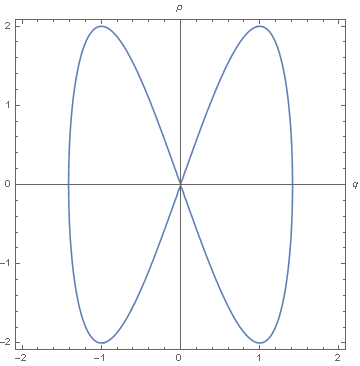
\includegraphics[scale=0.4]{Duffin}
 		\caption{Traiettoria nello spazio delle fasi per $E=0$}
 \label{Duffin}	
 \end{figure}
 	La traiettoria imperturbata è quindi:
 	\[\dv{q}{t}=\f{p}{2}=\sqrt{2q^2-q^4}	\]
 	 \[t-t_0=\int\f{1}{\sqrt{2q^2-q^4}}\d q\]
 	 Adesso sostituisco $q\rightarrow \sqrt{2}\sin(k)$:
 	 \[t-t_0=\int	\f{1}{2}\f{1}{\sqrt{\sin(k)^2-\sin(k)^4}} \sqrt{2} \cos(k) \d k=\int \f{1}{\sqrt{2}\sin(k)}\d k=\]\[=\f{1}{\sqrt{2}}\int \f{\sin^2\left(\f{k}{2}\right)+\cos^2\left(\f{k}{2}\right)}{2\sin\left(\f{k}{2}\right)\cos\left(\f{k}{2}\right)}=	\f{1}{2^\f{3}{2}}\int \tan\left(\f{k}{2}\right)+\cot\left(\f{k}{2}\right)\d k\implies\]
 	 Ora uso un po' di trigonometria per riesprimere tutto in funzione di $q$:
 	 \[t-t_0=\f{1}{\sqrt{2}}\ln\left|\tan\left(\f{k}{2}\right)\right|=\ln\left|\f{-1-\sqrt{1-\left(\f{q}{\sqrt{2}}\right)^2}}{\f{q}{\sqrt{2}}}\right|=\f{1}{\sqrt{2}}\text{settsech}\left(\f{q}{\sqrt{2}}\right)\]
 	 
 	 Infine\[q={\sqrt{2}}\sech({\sqrt{2}}\left(t-t_0\right))		\]
 	 
 	 e \[p=2\sqrt{2q^2-q^4}=4\sqrt{\left(\f{1}{\cosh({\sqrt{2}}\left(t-t_0\right))}\right)^2-\left(\f{1}{\cosh({\sqrt{2}}\left(t-t_0\right))}\right)^4}=4\sech^2\left(\sqrt{2}(t-t_0)\right) \sinh(\sqrt{2}(t-t_0))		\]
 	 La perturbazione che voglio mettere è \[V=q\cos(\omega_0 t)\]
 	 Quindi si ha, applicando la formula \ref{Melnikov} :
 	 \[D=\epsilon\int_{-\infty}^{\infty}	\cos(\omega_0 t)\f{p(t)}{2}\d t=\epsilon\int_{-\infty}^{\infty}	\cos(\omega_0 t)2\sech^2\left(\sqrt{2}(t-t_0)\right) \sinh(\sqrt{2}(t-t_0))		\d t	\]
 Questo schifo si fa con i residui (più incasinati del solito, visto che $\sech^2$ ne porta un numero infinito, quindi c'è una serie geometrica da risommare, credo), però non ho voglia di fare i passaggi, quindi riporto il risultato che è :
 \[D=\epsilon \pi \omega_0		\sin\left({\omega_0 t_0}\right)			\sin\left({\omega_0 t_0}\right)		\sech\left(\f{\pi\omega_0}{2^\f{3}{2}}\right)	\]
Come predetto, ci sono infinite intersezioni al variare di $t_0$, cioè del punto in cui calcolo la distanza di Melnikov, ad esempio per $t\ra\infty$, che consiste nell'avvicinarsi all'origine lungo $H^+$.

\end{exmp}
\subsection{Criterio di Chirikov}
Questo non mi è troppo chiaro, e anche la letteratura pare dire che sia un po' abusivo: prendo l'Hamiltoniana della standard map e la scompongo in Fourier
\[H=\f{I^2}{2}	+K\cos(\theta)	\sum_{m=0}^{\infty} \delta(t-2\pi m)=	\]
\[H=\f{I^2}{2}	+K\cos(\theta)	\sum_{n=0}^{\infty} \cos(nt)=	\]
A questo punto $K$ la vedo come perturbazione e guardo solo una risonanza, quella con $n=0$. \\Nell'Hamiltoniana imperturbata, le frequenze erano $\omega=I$, quindi le risonanze si hanno per $I=n$.
Dato che sto guardando la risonanza con $n=0$, mi concentro sulla traiettoria che ha $I=0$ (in $\theta=0$).
\[H=\text{const}=H(I=0,\theta=0)=K=\f{I^2}{2}	+K\cos(\theta)	\]
Da cui si ha che $I$ varia da $0$ a $2\sqrt{K}$ in una traiettoria (il fatto che $I$ non sia costante è dovuto unicamente all'aggiunta della perturbazione ed infatti va a $0$ per $K=0$).
Il problema sorge quando il $K$ diventa così grosso che questa traiettoria va a toccarsi con quella dell'altra risonanza, che ha $I=1$; lo spessore di quanto varia l'altra $I$ lungo una traiettoria è sempre circa $2\sqrt{K}$, quindi si toccano quando la somma dei due spessori è la pari alla distanza fra le due $I$ di risonanza, cioè $1$.
In definitiva, ottengo:
\[1=2\cdot 2\sqrt{K}\implies K=\f{1}{16}\]
Voglio generalizzare quest'idea per trattare un generico oscillatore e capire quando si genera il Chaos. L'unica richiesta è che l'oscillatore non sia lineare, in modo tale che la frequenza vari con l'ampiezza del moto (se non ho una dipendenza da $I$ non posso avere più risonanze).\\
Supponiamo quindi di avere un oscillatore sotto l'effetto di una forzante.
\\Il pezzo perturbativo, nelle variabili azione-angolo, va scomposto alla Fourier in $\theta$. Supponiamo inoltre che sia periodico nel tempo con frequenza $\Omega$;  quindi si può scomporre in Fourier anche la parte temporale in termini del tipo $e^{ik\Omega t}$
\[H=H_0+\sum_{a,b\in\mathbb{Z}^2} V_{a,b}(I) e^{ia \theta+ib\Omega t} \]
Voglio studiare una risonanza. La frequenza di $\theta$ è
\[\omega(I)=\left.\pdv{H_0}{I}\right|_{I=I_r}	\]
(calcolata nel punto $I=I_r$).
La condizione di risonanza è
\[\f{\omega(I)}{\Omega}\in\mathbb{Q}\quad	\f{\omega}{\Omega}=\f{k}{l}\quad k,l\in\mathbb{N}	\]
E supponiamo sia verificata per una certa $\omega(I_r),k,l$, con $l,k$ presi \textbf{coprimi}.\\
Faccio un cambio di variabili che rende la variabile angolo costante all'ordine $0$ e trasla il suo impulso coniugato in modo che sia nullo nel punto della risonanza. (cioè il nuovo impulso deve essere $J=\alpha(I-I_r)$).
\\Inoltre voglio riscalare $\omega$ in modo tale che $\omega'=\omega l$, in modo da semplificare il valore del suo rapporto con $\Omega$.
\\Dato che $\omega'=\pdv{H_0}{J}$, basta riscalare $J=\f{I-I_r}{l}\implies I=lJ+I_r$. Dette $\psi,J $ le nuove variabili, la generatrice che fa queste trasformazioni sarà della forma
\[F(\theta,J)=\theta(lJ+I_r)+f(J)\]
in modo che \[I=\pdv{F}{\theta}=lJ+I_r\]
Per quanto riguarda la trasformazioni sugli angoli, si vuole il nuovo angolo $\psi$ costante del tempo (all'ordine $H_0$), quindi
\[\psi=l\theta-k \Omega t\]
Questa trasformazione fa il lavoro, ricordando che $\theta(t)=\omega t $ e $l\theta-k\Omega=0$.
\\Con quest'ulteriore richiesta si trova $f$ e quindi la generatrice $F$:
\[F=(l\theta-k\Omega t)J+\theta I_r			\]
Il cambiamento nell'Hamiltoniana è

\[\psi=l\theta-k\Omega t\quad J=\f{I-I_r}{l}\quad H(J,\psi,t)=H_0(J)+V+\pdv{F}{t}=H_0+\sum_{a,b\in\mathbb{Z}^2} V_{a,b}(I) e^{\f{i}{l}[a \psi+k a\Omega t+b l\Omega t]}-k\Omega J		\]

$\psi$ varia molto poco durante un periodo di $\Omega$ (Le variazioni sono all'ordine di $V$), di conseguenza si può fare la media temporale dell'Hamiltoniana in un tempo  $t=\f{2\pi}{\Omega}$, che fa sparire tutti i termini di Fourier in $\Omega$ tranne quelli con coefficiente di $\Omega$ pari a $0\implies ka=-lb$.
Se $ka =-lb$ e $k,l$ sono coprimi, vuol dire che devo guardare tutti le $a,b$ per cui, preso $p$ intero, $a=lp$ e $b=-kp$.Dato che il potenziale di partenza era reale, $V_{a,b}=V_{-a,-b}$ (ogni volta che inverto $a$ o $b$ prendo un coniugato, se li inverto entrambi ritorno a $V$), quindi posso sommare le coppie $\pm p$ nella sommatoria e considerare solo i $p\ge0$.\\Non c'è nessun termine per $p=0$, perchè dipenderebbe solo da $J$ e potrebbe essere riassorbito nella definizione di  $H_0$.
\[\bar{H}=H_0+2\sum_{p=1}^{\infty} V_{lp,-kp}(I) \cos\left({{ip} \psi}\right)-k\Omega J	\]
Di questa serie faccio un'approssimazione brutale e prendo solo $p=1$, inoltre  dato che $J$ varia solo al prim'ordine in $V$ ( in realtà si vedrà che varia come $\sqrt{V}$, ma l'importante è che la variazione vada a $0$ per $V\rightarrow0$), posso espandere $H_0$ (visto che $V$ è già al prim'ordine) in Taylor intorno allo 0 di $J$ (è dove sta la risonanza), ottenendo l'equazione del pendolo.
\[H\approx H_0(I=I_r)+\left.\pdv{H_0(I)}{\f{I-I_r}{l}}\right|_{I=I_r} J+\left.\pdv[2]{H_0(I)}{\f{I-I_r}{l}}\right|_{I=I_r} \f{J^2}{2}	+ 2V_{l,-k}(I=I_r) \cos\left({{ip} \psi}\right)-k\Omega J=	\]
Ignoro il termine costante $H_0(I_r)$ che non cambia il moto e ricordo che $\omega=\pdv{H_0}{I}$:
\[H\approx l \omega J+l^2	\left.\pdv[2]{H_0(I)}{I}\right|_{I=I_r} \f{J^2}{2}+ 2V_{l,-k}(I=I_r) \cos\left({{ip} \psi}\right)-k\Omega J	\]
Nell'ultimo passaggio uso la condizione di risonanza\[	\f{\omega}{\Omega}=\f{k}{l}\]
\[H\approx   l^2	\left.\pdv[2]{H_0(I)}{I}\right|_{I=I_r} \f{J^2}{2}+ 2V_{l,-k}(I=I_r) \cos\left({{ip} \psi}\right)\]
Che è proprio l'equazione di un simil-pendolo, la cui separatrice (che individua la regione di tori invarianti, cioè di moti limitati) è
\[H=2V_{l,-k}\implies J=\sqrt{\f{8 V_{l,-k}}{l^2\pdv[2]{H_0}{I}}}\cos\left(\f{\psi}{2}\right)\]
Da cui la variazione di $J$ è, in generale (uso $H=const=0$, $J=0+\Delta J$):
\[\Delta J=	\f{2}{l}\sqrt{\f{2 V_{l,-k}}{\pdv[2]{H_0}{I}}}\implies \Delta I=2\sqrt{\f{2 V_{l,-k}}{\pdv[2]{H_0}{I}}}	\]
La formula che volevo era per la variazione della frequenza in un periodo, che si ottiene con $\Delta \omega\approx \pdv{\omega }{I }\Delta I$.\\Ricordo inoltre che $\omega=\pdv{H_0}{I}$:
\boxedeq{Chiri}{\Delta \omega=2\sqrt{{2 V_{l,-k}}{\pdv{\omega}{I}}} }
La condizione di Chirinkov è semplicemente che le $\omega$ di due diverse risonanze si "tocchino"; avendo fatte trentamila approssimazioni, questo risultato sarà solo indicativo.
	\section{Sistemi dissipativi}
Sono sistemi in cui non si conserva l'energia e lo spazio delle fasi si contrae. Detto in altri termini, essendo $J$ lo Jacobiano della trasformazione temporale ad un certo tempo $t$, si ha:
\[\det(J)<1\]
Il fatto che si sia una contrazione del sistema, non impedisce certamente la formazione di Chaos. Per fare un esempio, in un sistema $3D$, una certa palla di condizioni iniziali può essere contratta fino a diventare una retta (nel migliore dei casi, il sistema può anche tendere a un frattale), a cui poi uno può far fare ogni tipo di "caotica" traiettoria.
\begin{defn}[attrattori]
	Un qualunque set di punti a cui tende la dinamica del sistema, ad esempio nel caso \ref{limit}, l'attrattore è il cerchio limite.
	
\end{defn}
Notare che per avere un attrattore lo spazio delle fasi deve intuitivamente contrarsi,  quindi è necessario avere un sistema dissipativo.

\subsection{Biforcazione di Hopf}
Qualitativamente è un fenomeno che si trova studiando un punto stabile al variare di un parametro.
Supponiamo il moto del tipo:
\[\dv{\vec{z}}{t}=\vec{F}(\vec{z},R)\]
Ad esempio, il moto di un fluido al variare del numero di Reynolds.
Studiando un punto fisso per ogni $R$, può capitare che i suoi autovalori, supposti quelli di una spirale stabile, cioè del tipo
\[\lambda_\pm(R)=\alpha\pm i\beta	\quad \alpha<0	\]
al variare di $R$, abbiano che la loro parte reale (che decreta la stabilità del punto) ruotk nel piano complesso, passando da $\alpha<0$ ad $\alpha>0$, rendendo il punto instabile.
\\Sotto alcune condizioni può infine capitare che le orbite intorno al punto, ormai diventate instabili, tendano invece ad un cerchio limite intorno al punto. Visivamente si può immaginare questo fatto come la dinamica di una doppia buca in $3D$ generata dalla rotazione intorno all'asse $y$ della funzione:
\[y=-\lambda x^2+ x^4\]
Per $\lambda<0$, l'origine è un punto stabile, mentre , quando $\lambda$ diventa $>0$, i punti di minimo si rompono in $\pm\sqrt{\lambda}$ (che ruotati intorno all'asse $y$ lungo il piano $x-z$ formano un cerchio limite) e l'origine diventa instabile.


\part{Econofisica}
\begin{defn}[arbitraggio]
Si dice che in un mercato è presente \textbf{arbitraggio} se è possibile guadagnare istantaneamente denaro (ad esempio comprando e rivendendo beni in posti diversi).



\end{defn}
L'assenza di arbitraggio è un'ipotesi fondamentale di tutta la teoria matematica per l'economia; questa può venire violata, ad esempio, se qualcuno si mette a fare insider-trading (ovvero nasconde delle informazioni per guadagnarci); non a caso la pena per questo reato è in genere pesantissima .
\begin{defn}[Martingale]\label{Martina}
Una sequenza di variabili casuali è detta \textbf{Martingale} se il valore di aspettazione dell'ultimo variabile è pari al valore della precedente. 
\end{defn}
Un esempio è il moto Browniano: ad ogni step posso muovermi in ogni direzione con uguale probabilità, quindi il valore di aspettazione della mia posizione è pari alla posizione allo step precedente.
\begin{defn}[Mercato efficiente].
	Il 	\textbf{Mercato efficiente} è un tipo di mercato che rispetta le seguenti proprietà
	\begin{itemize}
		\item Informazione libera (tutti gli operatori hanno le stesse informazioni$\rightarrow$ NO insider trading)
		\item Liquidità infinita : si può vendere e acquistare senza problemi
		\item  Poco attrito, ovvero trascurabili costi per le transazioni
	\end{itemize}




\end{defn}
Sulla base di queste ipotesi, Samuelson dimostrò, nel 1965 che i prezzi seguono una martingale; come conseguenza, questi sono un processo di Markov.
L'idea è mostrare che il prezzo attuale, con tutte le informazioni più recenti, contiene tutta l'informazione necessaria a predire la forma della distribuzione dei prezzi allo step successivo.\\

Se il prezzo è un processo di Markov, deve poter essere descritto da un'equazione del tipo Langevin. \\Empiricamente si osserva che i prezzi seguono, in media, una distribuzione esponenziale, del tipo $e^{\mu t}$; questo è anche dovuto al fatto che le banche offrono investimenti sicuri (senza perdite) con tasso di interesse $\mu$; quindi dopo un tempo $t$, il prezzo $S$ di un'azione aumenterà di \[\d S=\mu S\d t		\]
 Questa è la parte deterministica di incremento; va aggiuno un pezzo randomico alla Langevin:
 \[\d S=\mu S \d t+\sigma S \d \omega		\]
Dove $\d \omega= \omega(t+\d t)-\omega(t)$ è una variabile casuale con media 0 e varianza $\d t$. Il fatto che l'aumento è proporzionale ad $S$, rende conveniente passare alla variabile $\ln S$. Per cambiare i differenziali bisogna ricorrere alla \textbf{Formula di Ito} \ref{ito}
\[\d \ln(S)=\f{1}{S}\d S-\f{1}{S^2}\left(\d S\right)^2=\mu \d t+\sigma \d \omega-\f{1}{S^2}(2\sigma S)	^2 \d t=\left(\mu-\f{1}{2}\sigma^2\right)\d t+\f{1}{2}\sigma\d \omega\]
Questa roba è facile da integrare: è proprio l'equazione \ref{Browniano} (con un termine di drift che trasla il valor medio di $\left(\mu-\f{1}{2}\sigma^2\right)t$).\\
Rifaccio i passaggi visto che non me li ricordo; sia $R=\ln(S)+\left(\mu-\f{1}{2}\sigma^2\right)t$ la variabile casuale con distribuzione $P(R,t)$: per tempi piccoli di salto $\d t $ posso espandere in Taylor la $P$, sia $\phi(\omega,t) $ la distribuzione di probabilità del saltino di $\omega$:
\[P(R, t+\d t)=\int \left(P(R-\omega,t)  \f{1}{2}\sigma^2\phi(\omega)\right)\d \omega \approx\int\left( P(R,t) -\pdv{P}{R} \omega+\f{1}{2}\pdv[2]{P}{R}\omega^2\right)	\phi(\omega)\d 	\omega=	\]
Per ipotesi $\phi$ ha media nulla e varianza pari a $\d t$, quindi:
\[P(R,t+\d t)=P(R,t)+\f{1}{2}\pdv[2]{P}{R}\d t		\]
\[\partial_t P=\f{1}{2}\sigma^2\partial^2_R P\]
Che implica che la $P$ ha distribuzione (la condizione iniziale è una $\delta$ in $R=0$)\[P= \f{1}{\sqrt{2\pi}\sigma t} e^{-\f{R^2}{2 \sigma t}}\]
Da questa si vuole passare alla distribuzione per $S=e^{R+\left(\f{1} {2}\sigma^2-\mu\right)t}$:
\boxedeq{Geom}{P(S,t)=\f{1}{S} \f{1}{\sqrt{2\pi}\sigma t} e^{-\f{\ln(S)+\left(\mu-\f{1}{2}\sigma^2\right)t^2}{2 \sigma t}}	}
Dove si è assunto che al tempo $0$ $S$ valga $1$.
In generale, se la condizione iniziale è $S=S_0$ al tempo $t'$ basta sostituire\[S\rightarrow\f{S}{S_0}\quad	t\rightarrow t-t'\quad P\rightarrow \f{ P}{S_0}	\]
(cambio di variabile)

\[P(S,t)=\f{1}{S}\f{1}{\sqrt{2\pi}\sigma (t-t')} e^{-\f{\ln\left(\f{S}{S_0}\right)+\left(\mu-\f{1}{2}\sigma^2\right)(t-t')^2}{2 \sigma (t-t')}	}\]
La $\sigma$ prende il nome di \textbf{rischio} o \textbf{volatilità} ed è legata alla larghezza della distribuzione. \\Questa distribuzione è detta \textbf{ log-normale}, il moto che ne deriva (da un sampling) è detto moto geometrico-Browniano.
\section{Mercato finanziario}
Qua bisogna dare un mucchio di definizioni:


\begin{defn}[Spot Price]
	È il prezzo di un bene (asset) $S(t)$, determinato dalla domanda e dall'offerta nel determinato istante di tempo che si va a guardare.
\end{defn}


\begin{defn}[Financial Market ]
	Luogo dove si scambia o investe denaro secondo alcune regole, in pratica è un mercato dove il bene è il denaro stesso
\end{defn}

Ci sono due tipi di transazione nel mercato finanziario:
\begin{defn}[Stock Exchange (SE)]
Transazione dove si comprano/vendolo titoli (azionari o obbligazionari) oppure valute straniere. È molto regolamentato $\rightarrow$ poca libertà $\rightarrow$ basso richio/guadagno


\end{defn}
\begin{defn}[Over The Counter (OTC)]
	È un tipo di transazione con regole molto più libere fissate da dei contratti vincolanti, che possono portare a guadagni (ma anche perdite) molto grossi.
\end{defn}
Per evitare grosse perdite nelle transazioni OTC, ci sono varie strategie; per prima cosa vanno definiti i vari tipi di rischi:
\begin{itemize}
	\item \textbf{Credit Risk} nel caso in cui un contratto non riesca a venire rispettato da una delle due controparti per mancanza di liquidità; tendenzialmente questa cosa non accade per transazioni sullo Stock exchange grazie alle stringenti regolamentazioni che ci sono
	\item \textbf{Operational Risk} Rischio di un qualche errore umano (o di un computer) in una transazione; è circa imprevedibile. Rientrano in questa categoria anche i casi di mancato controllo che portano a delle transazione non autorizzate (e quindi magari non supportate da abbastanza liquidità)
	\item \textbf{Market Risk} Fluttuazioni degli Asset price dovuti ad eventi imprevedibili (politica, crisi, etc.). Può essere \textbf{specifico} se riguarda solo alcuni tipi di asset (ad esempio l'immobiliare) o non specifico interessa più o meno tutti i settori del mercato.
\end{itemize}
Per ridurre il market risk specifico, si possono investire in tanti settori fra loro scorrelati; è noto come la varianza della media di tante variabili casuali va giù come $\sim \f{1}{\sqrt{n}}$.
\\Per gestire i rischi globali del mercato, si introducono nuovi beni detti \textbf{derivatives}, che sono fortemente anti-correlati con tutti gli altri beni (quindi, se questi scendono, il loro valore sale). Questa strategia prende il nome di \textbf{hedging}.
\section{Derivatives}
\subsection{Futures}
Sono dei tipi di contratto in cui ci sono due parti (che assumono i ruoli rispettivamente di \textbf{Short} e \textbf{Long Position}) che si mettono d'accordo in modo tale che, ad un tempo fissato $T$ detto \textbf{Delivery date}, la persona che ha la short position deve vendere un asset (che in questo contesto prende anche il nome di \textbf{underlying})all'altra persona, ad un prezzo fissato.
Questo prezzo è detto \textbf{delivery price}.
In pratica l'idea è che se il prezzo dell' underlying corrispondente al future scende, la persona che ha la short position potrà guadagnarci un po' di soldi perchè potrà venderla ad un prezzo più alto di quello di mercato, e quindi il valore del future salirà. In questo senso questo tipo di contratto è anticorrelato al valore dell'asset.\\I future sono molto ben regolamentati e, in realtà, servono perlopiù a regolarizzare il mercato; ad esempio la long position è tenuta a depositare  una frazione del denaro che serve per pagare il contratto, detta \textbf{margin} (che varia nel tempo con regole fissate, a seconda di quanto sale il prezzo dell'asset nel tempo) in modo tale da eliminare qualsiasi tipo di Credit Risk. I prezzi di questi contratto sono fissati dallo stock exchange
\subsection{Forward}
È un tipo di contratto  analogo al future, però meno regolamentato e, di conseguenza, lascia molto più spazio di manovra (e speculazione)
\subsection{Options}
Sono un tipo di contratto ancora più libero dei future; anche qui c'è un contratto venduto da una persona ad un'altra. Il contratto prevede il diritto, per chi lo compra (detto \textbf{holder}, perchè mantiene l'opzione), di vendere (\textbf{put option}) o comprare (\textbf{call option}) un certo underlying ad un tempo $T$ (\textbf{expiry date}). Il prezzo per questo asset è detto \textbf{strike price} (o \textbf{exercise}).\\In realtà, esistono millemila varianti di opzioni, questa qui, la più semplice di tutte, prende il nome di \textbf{European option} (ed è stata la maggior responsabile edlla crisi in olanda a causa della bolla dei tulipani nel 1637, per questo venne abbandonata per qualche secolo).
\\La teoria di Black-scholes formula un'equazione differenziale per dare un prezzo sensato alle opzioni, e in realtà funziona per molte derivative che soddisfino certe ipotesi.\\
Bisogna anzitutto definire alcune quantità matematiche con cui lavorare. Si chiama \textbf{Portfolio} la quantità di denaro che è necessario investire per fare alcune operazioni (ovvero un bilancio fra il comprare/vendere asset o opzioni al tempo $t$) e lo si indica con $\Pi(t)$.
Sia invece $C(t)$ il costo di un contratto di call option venduto al tempo $t$ che scada dopo un'expiry date fissata $T$ con exercise $K$. Invece $S(t)$ è il valore istantaneo dell'underlying (lo spot price) e $P(t)$ è il costo di un contratto di put option.


	
\subsubsection{Put-Call parity}

C'è una relazione fra $S$, $C\econg P$:
supponiamo di fare la seguente operazione: al tempo $t$ compriamo un underlying ed un contratto di call option e vendiamo a qualcuno il diritto di put option (entrambi con lo stesso strike price $K$).
\\Il portfolio necessario a queste operazioni è
\[\Pi=S+P-C	\]
All'expiry date $T+t$, ci sono vari casi:
\begin{enumerate}
	\item Se il valore dell'asset è $S<K$ allora sarà conveniente comprare un underlying dal mercato per un prezzo $S$, e venderlo  prezzo $K$, a chi ci ha dato il diritto di put option, con un ricavo \[K-S\] mentre il tizio a cui abbiamo venduto la call option non farà niente, sennò ci perderebbe. In questo caso al tempo $t+T$ avremo un denaro:
	\[S+K-S-(0)=K\]
	\item Nel caso opposto, cioè $S>K$, non eserciteremo il diritto di put, ma dovremo vendere la nostra azione $S$ comprata all'inizio a chi ha comprato la nostra call per un valore $K$, quindi alla fine ci ritroveremo in mano $K$ soldi.
\end{enumerate}
Quindi, in entrambi i casi, il portfolio $\Pi$ si traforma in $K$ soldi alla fine. Questa quantità deve essere esattamente uguale a quanto ci frutterebbe depositare quel denaro in banca, cioè 
\[\Pi\rightarrow\Pi e^{(T-t)\mu}=K\implies \Pi=Ke^{(t-T)\mu}	\]
Se questa roba non fosse vera, ci sarebbe arbitraggio. La relazione prende quindi la forma:
\[S(t)+P(t)-C(t)=K e^{\mu(t-T)}	\]

Adesso è ora di ricavare la generica equazione di Black-Sholes. Indichiamo il prezzo di un'opzione generica (cioè che può essere sia di tipo put che call) venduta al tempo $t$ con $O(S,t)$. Ovvero questo prezzo dipenderà in generale dal tempo $t$ e poi dal valore dell'underlying (che è una variabile casuale!) a quel tempo.
\\Si ha, dalla formula di Ito:

\[\d O= \pdv{O}{t}\d t +\pdv{O}{S} \d S+\f{1}{2}\pdv[2]{O}{S} \d S^2= \left(\pdv{O}{t}+\pdv[2]{O}{S} S^2 \sigma^2\right)\d t +\pdv{O}{S}  \d S		\]
Per ottenere le equazioni generica di Black e Sholes supponiamo di avere un contratto $O$ il cui valore deve essere in ogni istante uguale a quello di un'altro generico investimento sul mercato con lo stesso valore. Il più generico investimento ha la forma:
\[\Pi(t)+\Delta(t) S(t)		\]
dove $\Pi $ sono soldi investiti in un fondo sicuro (con rate di crescita assicurato $r$ e $\Delta\in[0,1]$ è una frazione dell'asset $S$ (dato che il contratto $O(S,t)$ riguarda un singolo asset, $\Delta$ non può essere più di uno, altrimenti i due valori non potrebbero mai essere uguali).
Si deve avere quindi in ogni istante 
\[O=\Pi+ S\Delta 		\]
Supponiamo che ad intervalli infinitesimi di tempo $\delta t$ il valore dei titoli cambi secondo le leggi del mercato, l'aumento infinitesimo di $\Pi$, visto che è un fondo sicuro, è $\Pi r \d t$, mentre l'aumento di $S$ è $\d S$.
\[\d O=	\Pi r \d t+\Delta \d S=\left(\pdv{O}{t}+\f{1}{2}\pdv[2]{O}{S} S^2 \sigma^2\right)\d t +\pdv{O}{S}  \d S	\]
Da cui 
\[\Pi =\f{1}{r}	\left(\pdv{O}{t}+\f{1}{2}\pdv[2]{O}{S} S^2 \sigma^2\right)	\quad \Delta=\pdv{O}{S}  	\]
Questa è la condizione che, \textbf{in modo deterministico}, ad ogni istante di tempo il valore di $O$ e di un certo denaro investito inizialmente restino uguali.

Il significato di questo ragionamento è che chi vende $O$ può usare il denaro ottenuto per comprare il portfolio $\Pi+\Delta S$ e azzerando il rischio (ma anche il guadagno! altrimenti ci sarebbe arbitraggio).
Rimettendo tutto nella prima equazione:
\boxedeq{BS}{O=S\pdv{O}{S}+\f{1}{r}	\left(\pdv{O}{t}+\f{1}{2}\pdv[2]{O}{S} S^2 \sigma^2\right)}
La differenza nelle varie opzioni sta nelle condizioni al contorno (ne servono $2$); una di queste è fissata allo scadare del contratto, quando è noto il valore di $O$, l'altra la si trova dall'andamento asintotico.
\begin{obs}
L'algoritmo di investire i soldi di $O$ per non perdere soldi funziona, ma è inutile perchè alla fine della giornata nessuno ci guadagnerebbe; realisticamente ci si discosta un pochino dall'algorirmo (quindi dal $\Delta=\pdv{O}{S}$) aumentando in modo infinitesimo il rischio e generando un possibile margine di guadagno
\end{obs}
\subsubsection{Forma adimensionale}
Vogliamo risolvere l'equazione \ref{BS} nel caso di call option.\\Per questo contratto le condizioni al bordo, all'expiry date (che fissiamo in $t=0$) sono:
\[O=C=\max\left(S-K,0\right)			\]
Questo perchè, se $S$ vale più di $K$, uso la call per comprarlo ad un prezzo $K$ e rivenderlo ad $S$, altrimenti non uso il mio diritto.
Le altre condizioni asintotiche, per $S=0$ sono $C=0$ (se $S=0$, allora resta $0$ e il mio contratto di call non vale niente) e $C=S-K\sim S$ per $S\rightarrow\infty$ (dove per infinito si intende grosso rispetto $K$).\\
A questo punto ho una scala di prezzo, $K$ (quindi $S\rightarrow K s$), mentre per la scala di tempo uso $\f{\sigma^2}{2}\propto \f{1}{t}$, inoltre inverto la direzione del tempo $t\rightarrow-t$ in modo tale da risolvere l'equazione per $t\ge0$:
\[rO=rs\pdv{O}{s}-\f{\sigma^2}{2}\pdv{O}{\tau}+\f{\sigma^2}{2}\pdv[2]{O}{s} s^2 \]
Inoltre come al solito conviene passare da $s\rightarrow x=\ln(s)$:
\[\f{2r}{\sigma^2}O=\f{2r}{\sigma^2}\pdv{O}{x}		-\pdv{O}{\tau}+\pdv[2]{O}{x} -\pdv{O}{x} 	\]
L'unico parametro che ho è quindi l'adimensionale $\kappa=\f{2r}{\sigma^2}$
\[\kappa O+\pdv{O}{\tau}-\pdv[2]{O}{x}+\pdv{O}{x}	(1-\kappa)	=0\]
con le condizioni al bordo:
\[O(x\rightarrow\infty)\sim e^x		\quad O(t=0)=\max\left(e^x-1,0\right)\quad O(x\rightarrow-\infty)=0\]
L'equazione si può trasforma in un'equazione di diffusione con la sostituzione:
\[O=e^{\f{1-\kappa}{2}x-\left(\f{1+\kappa}{2}\right)^2	\tau			}g(x,\tau)\]
\[\pdv{g}{t}=\pdv[2]{g}{x}\]
\subsection{Risk-Neutral valuation}
Si può verificare per sostituzione che vale
\[\f{C(t)}{e^{rt}}=E^*[\f{C(T)}{e^{rT}}]			\]
dove la media $E^*$ è fatta con una geometrica-Gaussiana a drift nullo (il valore di aspettazione di $C(T)$ è determinato da quello di $S(T)$, che è una variabile casuale).
\\In realtà questo risultato è frutto di un teorema generale che afferma che il prezzo giusto per una derivative è dato dal valore di aspettazione del suo valore scontato nel tempo calcolato sotto una martingale equivalente.\\ Prendere un prezzo scontato vuol dire dividerlo per l'incremento certo che si avrebbe usando un portfolio a rischio nullo (in questo senso $r$ è universale, sennò ci sarebbe arbitraggio) e prendere una martingale equivalente vuol dire cambiare la misura di probabilità con una equivalente in modo tale che il processo scontato diventi una martingale. In questo caso il valore di $\tilde{C}$ cioè della call option scontata, rispetta la martingale equivalente $\d \tilde{C}=\sigma \tilde{C}(t)\d W^*$.\\Il teorema di Girsanov dà la forma della nuova misura di probabilità da usare, tramite derivata di Radon-Nikodym.
\[\d W^*=\gamma(t)+\d W		\]
Sia $\mu$ la nuova misura e $\nu$ la vecchia (secondo cui $\d W$ è di Wiener).
\\Allora la derivata è
\[\pdv{\mu}{\nu}=\exp(-\int_0^t \gamma(x)\d W(x)-\f{1}{2}\int_0^t\gamma(x)^2\d x)=L(t)\]
(notare che giustamente $\ave{L}=1$)
\\L'ipotesi del problema è solo che $L$ sia rinormalizzabile, cioè $\exp(\f{1}{2}\int_0^t\gamma(x)^2\d x)$ sia finito.
\\Infine, $B(t)=e^{rt}$ (cioè il processo di guadagno deterministico) è detto numeraire. L'ipotesi del teorema è che non ci sia arbitraggio.
\section{Fatti in disordine}

Per piccoli intervalli di tempo $S$ è costante, la variazione di prezzo è gaussiana.\\
\textbf{Volatility smile}La volatilità varia nel tempo, come la misuro? (non posso fare medie se varia).\\Dal prezzo delle Option: varia a seconda dello strike price e dell'asset value! In particolare supponendo il prezzo dell'asset circa costante nell'intervallo di tempo considerato, cioè $\d S=S_0 \sigma\d W$  e supponendo la $\d W$ non gaussiana, ma somma di $N$ distribuzioni con curtosi $\ne 0$, posso calcolarmi la variazione del prezzo delle call usando il polinomi di Chebishev $Q_2$ (suppongo $Q_1$ nullo se la distribuzione $\d W$ è pari, come mi aspetto) e la curtosi diversa da 0. Si trova una correzione che va come
\[\Delta C(t)\propto\f{\hat{k}_4(K-S(t_0))^2}{\sqrt{T}\sigma^2S(t_0)^2}	e^{-\f{(K-S(t_0))^2}{2\sigma^2 S^2(t_0)T}}\]
Cioè va giù per tempi lunghi. Posso quindi trovare la nuova volatilità calcolata col "vecchio" prezzo della call:
\[\Delta C=\delta \sigma\pdv{C}{\sigma}\]
Si trova il volatility smile:
\[\delta \sigma\propto \hat{k}_4\f{(K-S(t_0))^2}{T}	\]
ovvero la volatilità cresce all'aumentare della differenza fra strike price e spot price e va giù con l'expiry date $T$.
\\\textbf{Scala dei prezzi} Variazione di prezzo dovuta a tante cause, moneta che varia, crescita economica , fluttuazioni random.\\Si possono considerare varie variabili per tempi brevi sono più o meno  equivalenti:differenza di prezzi, cambiamento di prezzi scontato (moltiplico per la deflazione che tiene conto della variazione della moneta), ritorno  (variazione in rapporto al valore del prezzo)[+=variazione percentuale;-=se cambio l'intervallod i tempo guardato cambia], logaritmo del ritorno più uno (incremento del logaritmo)[qui se cambio il tempo mi aspetto cambi linearmente, ma non è una relazione lineare]. Per tempi lunghi le cose cambiano.
\\\textbf{scala dei tempi} tempo fisico,del mercato (cioè tiene conto solo di quando sono aperti i mercati, all'apertura e chiusura fa casini), numero di transazioni.\\
\textbf{correlazioni, processi stazionari,asintoticamente staz o di ordine N}: nei mercati finanziari le correlazioni sono solo a tempi brevi, tempi lunghi=gaussiana ma la volatilità varia
\\\textbf{legge di scala della varianza}: du vase wigner per tempi da un giorno a 3 mesi, sotto i trent minuti $\sigma\propto t^{0.8}$ regime superdiffusivo\\Si studia la variazione nel tempo della volatilità, visto che il decadimento della correlazione a due punti non è così utile in processi non lineari (cioè varianza non lineare nei tempi), la  varianza è correlata anche a tempi lunghi come $t^{-0.3}$ circa
\\\textbf{processi infinitamente divisibili}: requisito come modello per i prezzi (distr uniforme non lo è, la $\Gamma$ sì, ad es), voglio distr leptocurtiche, t student, truncated levy, somma di gaussiane , Levy normale con $\alpha=1.4$,
Levy non ha varianza, student cambia con la scala e non è stabile, somma di gaussiane non ha una legge di scala( il processo è diretto dalla $P(\Omega)$ che dà la distribuzione del volume delle transazioni. Cosa vuol dire legge di scala? so che la varianza varia linearmente nel tempo , a varianza fissa posso trovare $P(0)$, la probabilità di tornare nell'origine e vedo come dipende dal tempo di osservazione.\\
Truncated Levy non è stabile ma tende dopo un po' ad una gaussiana, il numero critico da distribuzioni da sommare è $N=\propto\hat{k}_4\propto \lambda^{-\alpha}\f{1}{1-\alpha}$, perchè il polinomio di chebishev $Q_2 $ ha come prefattore $\f{k_4}{N}$
\\Per intervalli di tempo piccoli lo scaling è di Levy:
\[P(0)\propto t^{-\f{1}{\alpha}}			\]
compatibile con $\alpha=1.4$.
\\Unico problema del modello è che i parametri $\alpha,\gamma, l$ variano nel tempo ($l$ credo sia il cutoff, $\gamma$ è l'andamento della correlazione per la volatilità $\f{1}{t^{\gamma}}$)
\\Detto in altri termini, ci sono più eventi rari del previsto.
\\Modelli per volatilità variabile: garch e arch
\\ Garch (1,1)  e Arch(1) possono aggiustare curtosi e varianza della distribuzioni,  inoltre la correlazione sulla varianza decade su un tempo caratteristico $\tau^{-1}=\ln (\alpha+\beta)$ che può essere reso arbitrariamente lungo. In realtà si ha un decadimento a potenza di solito (con $\gamma\approx 0.3$), quindi $\tau$ lo si prende lungo (due mesi circa) per simulare questo fatto.
Per un ARCH semplice si ha che $\sigma^2\propto \f{1}{1-3\alpha_1^2}$, quindi $\tau$Non lo si può prendere arbitrariamente lungo

La legge di scaling non è buona  (scala come una gaussiana) ma ci becca sia per il limite gaussiano, sia cambiando scala dei prezzi (cioè il volume delle azioni scambiate). TUttavia, andando a guardare $\Delta t$ sopra il minuto, scazza.
\\Correlazioni nel portfolio e rischio: voglio minimizzare la volatilità, scrivo la volatilità come una forma quadratica dei vari prezzi
\[\sigma^2 t=Cov{S_i,S_j}\]
e cerco gli autovalori minimi, gli autovettori corrisponenti minimizzano il rischio
\[\Pi =\sum_i	w_i S_i		\] 
\[R^2=\sum_i	w_i \sigma_i w_j \sigma_j C_{ij}	\]
dove $C_ij$ è la correlazione, quindi in pratica è $w_i w_j Cov_{ij}$. ho il vincolo di avere una quantità di soldi limitata.\\ 
$C_{ij}$ è una matrice random? dalla distribuzione di autovalori di $C=\f{1}{L}G G^T$ (in generale $G_{ij}$ è NxL che contiene il valore dell'incremento del logaritmo prezzo $i$ al giorno $j$, $L$ è il numero di giorni osservati)si vedono degli outlyers, in particolare la RMT predice
\[Q=\f{L}{N}\quad\lambda_{\pm}=\left(1\pm\sqrt{\f{1}{Q}}\right)^2 \quad P(\lambda)=\f{Q}{2\pi}\f{\sqrt{(\lambda_{+}-\lambda)(\lambda-\lambda_-)}}{\lambda}			\]
Mischiando fra loro i dati (cioè per ogni $S_i$ scambio a caso i valori nel tempo in modo diverso, in modo tale da aggiungere randomicità) si ha accordo perfetto, quindi c'è dinamica nascosta. (il fit lo faccio al variare di $\lambda_\pm$)
\\Posso anche studiare la distanza media fra gli autovalori con il GOE, (distribuzione $\Gamma_0(x)$) o la Brody ($\propto s^\beta\exp(-Bs^{1+\beta})$)
La matrice di correlazione $P(\rho_{ij})$ ha media positiva, legata all'indice della borsa, cioè al fatto che i prezzi sono racchiusi in pochi indicatori
	\\\textbf{Spazi ultrametrici}: introduco una distanza $d_{ij}^2=\ave{(\tilde{S}_i-\tilde{S}_j)^2}=2(1-\ave{\rho_{ij}})$ (il tilde serve solo a dire che ho traslato $S_i$ per ottenere media nulla e varianza unitaria; $S_i$ è sempre l'incremento del logaritmo).Spazio ultrametrico=distanza triangolare più forte
		\[d_{ij}\le \max\{d_{ik},d_{kj}\}			\]
Posso costruirci il Minimal spanning tree(def albero che minimizza la somma di tutti gli archi): algoritmo di Kruscal, ho tanti punti e tante connessioni possibili $d_{ij}$, ogni volta aggiungo la più piccola possibile di quelle rimanenti, a patto che non crei loops, finchè il grafo non diventa un albero: struttura a clusters
\\Crash finanziari: il \textbf{drawdown } è la diminuzione percentuale fra un max locale e il successivo  minimo locale. Empiricamente, questi seguono una distribuzione espnenziale, tuttavia  le code scazzano: i tre crash dell'ultimo secolo dovrebbero avvenire con probabilità mille volte più bassa.\\La struttura generale che si osserva è a gradini(più oscillazioni): gradini sempre più stretti:non sono statistiche (tutti vendono)\\ SOrnette: considero l'Hazard rate $h(t)$ cioè la probabilità di fare un crash per unità di tempo, e lo scrivo in modo analogo ad una transizione di fase
\[h=\f{1}{(t-t_c)^\gamma}\left(B_0+B_1\cos(\omega\ln(t-t_c)+\phi)\right)\]

Inoltre assumo che $\mu\propto h$ quindi posso ricavarmi la distribuzione della media dei prezzi, e da lì controllo con i dati: c'è buon accordo, ma il tempo $t_c$ è  sovrastimato, gli esponenti $\beta=1-\gamma$ e $\omega$ non sono universali, e ci sono troppi parametri da fittare e non è detto che il crash ci sia davvero












\appendix
\section{Probabilità e definizioni elementari}
	\subsection{Densità spettrale}
\begin{defn}[ensemble]
	Quando si ha una variabile casuale reale dipendente dal tempo $x$, conviene introdurre il concetto di \textbf{ensemble}. Un ensemble è un insieme di tante copie del nostro sistema casuale. Supponendo di avere, ad esempio, $N$ copie; se la probabilità di avere il sistema nello stato $x$ al tempo $t$ è $p_{(x)}$, allora $n_{(x)}=p\arg{x} N$ di queste copie al tempo $t$ saranno proprio $x_i$, ovvero la probabilità di avere il sistema in un certo stato si traduce, con l'ensemble, nell'avere un certo numero di copie del sistema in quello stato. Indicizzo le varie copie del sistema con $x_i$. Ciascuna di queste copie ha una certa evoluzione temporale $x_{i\;(t)}$  che è \textbf{fissata}, perchè una copia del sistema nell'ensemble corrisponde, in pratica, ad una \textbf{possibile evoluzione del sistema }.\\
	Nell'esempio pratico di un segnale casuale (ad esempio del rumore), supponendo di osservare il segnale nel tempo $N$ volte, si avranno tanti campionamenti, ciascuno dei quali sarà indicato con $x_{i\:(t)}$. 
	\\In questo linguaggio, per avere il valor medio della variabile $x$ al tempo $t$, bisognerà fare una media \textbf{sull'ensemble} al tempo $t$:
	\[\ave{x\arg{t}}=\f{1}{N}\sum_{i=1}^{N} x_{i\:(t)}\]
	Per indicare la media sull'ensemble si userà il simbolo $\ave{\bullet}$
\end{defn}
\begin{obs}
	Il fatto che ogni elemento dell'ensemble dipenda da $t$ non ha nulla a che fare con la stazionarietà del processo; ovvero parlando di ensemble nel caso di processo stazionario si avrà comunque per il singolo elemento dell'ensemble (ovvero un singolo campionamento) dipendenza da $t$, il punto è che questa dipendenza sparisce ogni volta che si fa la media sull'ensemble. 
	\\Un'altra importante considerazione da fare nel caso di processo stazionario è che fare la media sull'ensemble (non importa l'istante di tempo in cui la si fa, il processo è stazionario) e fare la media temporale di un \textbf{singolo elemento dell'ensemble} è equivalente per sistemi ergodici. Un sistema ergodico è un sistema che, dopo abbastanza tempo, "visita" tutte le sue possibili configurazioni. Nel caso di un sistema ergodico, quindi, basta avere anche solo \textbf{una} copia del sistema, che mediata per abbastanza tempo sarà equivalente ad avere un ensemble.
\end{obs}
\begin{exmp}
	Ora conviene dare un esempio pratico di ensemble nel caso di processo stazionario. 
	\\Il nostro ensemble sarà indicizzato da un parametro continuo (nel limite in cui si è ha un ensemble infinito questa è una buona modellizzazione) $\phi\in[0,2\pi]$; ogni singolo elemento dell'ensemble sarà quindi pesato con  $\f{\d \phi}{2\pi}$. 
	\\L'elemento $\phi$ dell'ensemble sarà $x_\phi$  definito da:
	\[x_{\phi\:(t)}=\cos(\omega t+\phi)		\]
	Questo ensemble è stazionario perchè,campionando ad un istante di tempo $t$ fissato, la distribuzione di probabilità per $x$ è indipendente dal tempo. \\
	Mostriamolo con i conti: la probabilità è associata al peso nell'ensemble, cioè $|\d \phi| \frac{1}{2\pi}$
	\[x=\cos(\omega t+\phi)	\implies\d x= \sin(\omega t +\phi)\d \phi=\sqrt{1-x^2}\d \phi	\]
	\[\d p\arg{x}= \frac{|\d \phi|}{2\pi}=\frac{|\d x|}{2\pi \sqrt{1-x^2}}\implies W\arg{x}=\f{1}{2\pi \sqrt{1-x^2}}\]
	Una volta campionato il segnale in un istante di tempo, misura che seguirà la distribuzione appena ottenuta, il segnale successivo sarà determinato  univocamente.
\end{exmp}
\subsection{Densità spettrale}
Supponiamo ora di avere un processo stazionario e di considerare un elemento dell'ensemble $x_{(t)}$. Si possono definire media quadratica temporale e distribuzione spettrale per questo processo.
Facendo la media quadratica su un intervallo di tempo $2T$ bisogna poi dividere per l'ampiezza dell'intervallo. Dato che si immagina di avere oscillazioni molto più rapide del tempo di misura, si prende il limite $T\rightarrow \infty$; la notazione per le medie temporali (diverse da quelle sull'ensemble) è $\bar{\bullet}\:\:$:
\[\bar{{x^2}}=\lim_{T\rightarrow\infty}\frac{1}{2T} \int_{-T}^{T} x^2\arg{t}\d t		\]
Se il sistema è ergodico è equivalente fare medie temporali o su ensemble,e si ha:
\[\bar{{x^2}}=\ave{x^2}\]
Vorremmo trovare come l'energia (che si suppone proporzionale a $x^2$) è distribuita in frequenza.
Per farlo, vorrei usare il teorema di Parseval su $x\arg{t}$: il problema è che questa funzione non è a quadrato integrabile; per sistemare le cose definisco \[x_{T\:(t)}=x\arg{t} \rchi_{[-T,T]\:\:(t)}		\]
dove $\rchi$ è la funzione caratteristica.
Allora $x_T$ è a quadrato integrabile, perchè a supporto compatto, quindi vale il teorema di Parseval:
\[\int_{-\infty}^{+\infty} x^2_T \d t=\f{1}{2\pi} \int_{-\infty}^{+\infty}	|\tilde{x}_{T\:(\omega)}|^2	\d \omega\]
dove $\tilde{x}_{T\:(\omega)}$ è la traformata di Fourier.
\[\tilde{x}_{T\:(\omega)}=\int_{-\infty}^{+\infty} x_T \;e^{i \omega t} \d t\]
Si ha allora:
\[  \bar{x}^2=\lim_{T\rightarrow\infty}\frac{1}{2T} \int_{-T}^{T} x^2\arg{t}\d t=\lim_{T\rightarrow\infty}\frac{1}{2T} \int_{-\infty}^{+\infty} x^2_{T\:(t)} \,\d t	=\lim_{T\rightarrow\infty}\frac{1}{2T} \int_{-\infty}^{+\infty}	|\tilde{x}_{T\:(\omega)}|^2 \d\omega		\]
Ed è naturale a questo punto definire la densità spettrale in potenza $S\arg{\omega}$ in modo tale che $\int_{-\infty}^{+\infty} S\arg{\omega} \d \omega=\ave{\bar{x^2}}$:
\boxedeq{spectraldensity}{S_{(\omega)}=\ave{\lim_{T\rightarrow\infty}\frac{1}{2T(2\pi)}	 	|\tilde{x}_{T\:(\omega)}|^2 }	}

\subsection{Funzione di Correlazione}
\begin{defn}
	Date due funzioni a quadrato integrabile si definisce la correlazione su un tempo $\tau$:
	\[G_{fg\:(\tau)}=\int_{-\infty}^{+\infty} \d t f(t)	g(t+\tau)\]
	che è sostanzialmente  il prodotto di convoluzione di $f\arg{-t}$ con $g\arg{t}$.
\end{defn} 
Dato che il la trasformata di Fourier del prodotto di convoluzione è il prodotto delle trasformate di Fourier delle due funzioni e che la trasformata di Fourier per funzioni $f$ reali ha la proprietà \[\mathcal{F}[f\arg{-t}](\omega)=\mathcal{F}[f\arg{t}]^*(\omega)\]
Si può scrivere allora:
\begin{equation}
\tilde{G}_{fg}=\mathcal{F}\left(\int_{-\infty}^{+\infty} \d t f(t)	g(t+\tau)\right)=\mathcal{F}\left(\int_{-\infty}^{+\infty} \d t f(-(-t))	g(t+\tau)\right)=
\end{equation}
L'argomento della trasformata di Fourier è la convoluzione di $f\arg{-t}$ e $g\arg{t}$, quindi la sua trasformata è il prodotto delle trasformate.
\begin{equation}
=\mathcal{F}[f\arg{-t}](\omega)\mathcal{F}[g\arg{t}](\omega)	=\tilde{f}^* \tilde{g}\label{corr}
\end{equation}

L'autocorrelazione di una funzione è definita come la funzione di correlazione della funzione $f$ con sè stessa.\\
Si vuole ora definire la funzione di autocorrelazione per il nostro elemento dell'ensemble; come prima c'è il problema che $x\arg{t}$ non è a quadrato integrabile; pertanto si passa alle medie temporali:
\[G\arg{\tau}=\lim_{T\rightarrow\infty}\frac{1}{2T}\int_{-T}^{T} \d t\: x\arg{t}x\arg{t+\tau}=\lim_{T\rightarrow\infty}\frac{1}{2T}\int_{-\infty}^{+\infty} \d t\: x_{T\:(t)}x_{T\:(t+\tau)}\]
Da cui utilizzando il fatto \ref{corr} si ottiene:
\[{\tilde{G}}=\lim_{T\rightarrow\infty}\frac{1}{2T} \tilde{x}_{T\:(\omega)}^*\tilde{x}_{T\:(\omega)}=2\pi S\arg{\omega}\]

Esplicitando l'antitrasformata di Fourier si ha l'importante relazione:
\boxedeq{Wiener}{G\arg{\tau}=\int_{-\infty}^{+\infty} S\arg{\omega} e^{-i \omega \tau}	\d\omega	}
e viceversa
\[S\arg{\omega}=\f{1}{2\pi}\int_{-\infty}^{+\infty} G\arg{\tau} e^{i \omega \tau}	\d\omega\]
\begin{exmp}[rumore bianco]
	Una variabile casuale del tipo di Wiener ha potere spettrale costante a tutte le frequenze
	\[\dv{ W(t)}{\d t}=\xi(t)\]
\[\ave{\xi(t)\xi(t+\tau)}=\delta(\tau)\implies|\tilde{\xi}(\omega)|^2=1\]

\end{exmp}
\begin{exmp}[rumore marrone]
è il rumore prodotto da un segnale casuale che è l'integrale di un processo di Wiener
\[A(t)=\int_{t_0}^t \d W(x) \quad \xi=\dv{A}{\d t} \quad \xi(\omega)=-i\omega A(\omega)\]
in trasformata si ha
\[\ave{\xi(\omega)\xi \Omega}=\ave{\omega^2 A(\omega)A^*(\omega)}=1\implies\ave{|A(\omega)|^2}=\f{1}{f^2}\]

Quindi va giù come  $\f{1}{f^2}$
\end{exmp}
\begin{exmp}[rumore rosa]
detto anche rumore $\f{1}{f}$, ha l'andamento tipico $\f{1}{f}$
	


\end{exmp}
Un processo è correlato a tempi lunghi se l'integrale della sua correlazione sul tempo diverge. \\
In questo caso, il valore di aspettazione di $\f{1}{\sqrt{N}}\sum_i x_i$ divergerebbe (perchè i doppi prodotti, che sono determinati dalla correlazione, divergono)


\section{Equazioni di Navier-Stokes}

L'equazione $\vec{F}=m\vec{a}$ per un fluido è:
\[\pdv{\vec{v}}{t}+\left(\vec{v}\cdot\vec{\nabla}\right)\vec{v}=-\f{\vec{\nabla} p}{\rho}+\nu \nabla^2 \vec{v}\]
Per un fluido incomprimibile, vale inoltre:
\[\vec{\nabla}\vec{v}=0\]
\section{Metodo delle caratteristiche}\label{nonhoidee}
Supponiamo di avere un'equazione \textbf{lineare} alle derivate parziali in due variabili (il caso più semplice, ma generalizzabile)
\[\pdv{z}{x} a(x,y,z)+\pdv{z}{y}b(x,y,z)=c(x,y,z)\]
La soluzione è una superficie in $\mathbb{R}^3$, parametrizzata da $x,y$:
\[(x,y,z(x,y))\]
I vettori tangenti a questa superficie si trovano differenziando rispetto ad $x$ o $y$, ad esempio
\[\left(\d x,0,\pdv{z}{x}\d x\right)\propto\left(1,0,\pdv{z}{x}\right)\]
Da cui si vede che il vettore normale ad entrambi ai vettori tangenti, e quindi alla superficie, è
\[\vec{t}=\left(\pdv{z}{x},\pdv{z}{y},-1\right)\]
Questo vettore è perpendicolare a
\[\left(a(x,y,z),b(x,y,z),c(x,y,z)\right)\]
perchè, facendo il prodotto scalare con il vettore normale, si ritrova l'equazione differenziale iniziale ( e quindi viene $0$).\\
Usando questa osservazione, si può trovare una soluzione particolare dell'equazione differenziale cercando una curva punto per punto parallela al vettore dato:
\begin{equation}
	\d \vec{\gamma}=\left(\d x,\d y,\d z\right)\quad\quad \f{\d x}{a}=\f{\d y}{b}=\f{\d z}{c}\label{strumentopolo}		
\end{equation}

parametrzzando la curva, ad esempio con $t$, si hanno le equazioni di \textbf{Lagrange-Charpit}.
\[\dv{x}{t}=a\quad\quad\dv{y}{t}=b\quad\quad \dv{z}{t}=c\]
Come fa uno a trovare la soluzione generale? Beh si parte da una condizione iniziale, che geometricamente è una curva  che sta nella superficie della soluzione (in caso di $\mathbb{R}^n$ è una $n-2$ varietà). Poi ciascun punto iniziale di questa curva fa parte di una diversa curva $\vec{\gamma}$ definita prima, che è soluzione dell'equazione differenziale; il risultato è la superficie della soluzione.\\Algebricamente il modo di procedere è il seguente: 
si risolvono le due equazioni \ref{strumentopolo}, ad esempio
\[ \f{\d x}{a}=\f{\d y}{b}\]
chiamando $u$ la costante di integrazione\footnote{La costante di integrazione descrive le varie condizioni iniziali da cui partono le curve, quindi variarla vuol dire andare a cercare le varie curve al variare del punto iniziale}, si ottiene qualcosa del tipo\[u= \int\f{\d x}{a}-\int \f{\d y}{b} 	\]
analogamente
\[v(x,y,z)= \int\f{\d z}{c}-	\int \f{\d y}{b}\]
Muovendosi sulla curva $\gamma$, sia $u$ che $v$ sono costanti (perchè rispettano le equazioni di Charpit), quindi viene rispettata l'equazione:
\[f(u,v)=0\]
o, equivalentemente 
\[u=f(v)\]
con $f$ \textbf{arbitraria}. (dato che $u,v$ sono costanti sulla curva $\gamma$ è chiaro che si può imporre una condizione del genere). Questa $f$ viene trovata imponendo le condizioni iniziali:
\[f(u(z(x,y_0),x,y_0),v(z(x,y_0),x,y_0))=0\]
Dato che si ha una soluzione che rispetta le condizioni iniziali e anche il movimento lungo $\gamma$, per definizione si ha la soluzione dell'equazione differenziale.
\\Per un esempio esplicito, guarda \ref{boh}.


\section{Trasformata di Mellin}\label{Mellin}
Data una funzione $f(x)$:
\[F(p)=\int_{0}^{\infty}	f(x)x^{p-1}\d x	\]
(questa cosa è lecita se questo integrale converge assolutamente)\\Come ogni trasformata, esiste l'inversa:
\[f(x)=\f{1}{2\pi i}\int_{c-i\infty}^{c+i\infty} \f{1}{x^p}F(p)	\d p		\]
Dove $c$ è un numero complesso che si trova in una fascia del piano complesso del tipo $\Re{z}\in[a,b]$, in cui $F(p)$ è analitica.
\end{document}
